%======================================================================
% Based on: University of Waterloo Thesis Template for LaTeX 
%======================================================================

% DON'T FORGET TO ADD YOUR OWN NAME AND TITLE in the "hyperref" package configuration below. 
% THIS INFORMATION GETS EMBEDDED IN THE PDF FINAL PDF DOCUMENT.
% You can view the information if you view properties of the PDF document.

% Contains options for print optimization, which I have commented out.

% Compile
% E.g. to process a thesis called "mythesis.tex" based on this template, run:

% pdflatex mythesis	-- first pass of the pdflatex processor
% bibtex mythesis	-- generates bibliography from .bib data file(s)
% makeindex         -- should be run only if an index is used 
% pdflatex mythesis	-- fixes numbering in cross-references, bibliographic references, glossaries, index, etc.
% pdflatex mythesis	-- it takes a couple of passes to completely process all cross-references

% N.B. The "pdftex" program allows graphics in the following formats to be included with the "\includegraphics" command: PNG, PDF, JPEG, TIFF
% Tip: Generate your figures and photos in the size you want them to appear in your thesis, rather than scaling them with \includegraphics options.
% Tip: Any drawings you do should be in scalable vector graphic formats: SVG, PNG, WMF, EPS and then converted to PNG or PDF, so they are scalable in the final PDF as well.
% Tip: Photographs should be cropped and compressed so as not to be too large.

% To create a PDF output that is optimized for double-sided printing: 
% 1) comment-out the \documentclass statement in the preamble below, and un-comment the second \documentclass line.
% 2) change the value assigned below to the boolean variable "PrintVersion" from " false" to "true".

%======================================================================
%   D O C U M E N T   P R E A M B L E
% Specify the document class, default style attributes, and page dimensions, etc.
% For hyperlinked PDF, suitable for viewing on a computer, use this:
\documentclass[letterpaper,12pt,titlepage,oneside,final]{book}
 
% For PDF, suitable for double-sided printing, change the PrintVersion variable below to "true" and use this \documentclass line instead of the one above:
%\documentclass[letterpaper,12pt,titlepage,openright,twoside,final]{book}

% Some LaTeX commands I define for my own nomenclature (template
\newcommand{\cmmd}[1]{\textbackslash\texttt{#1}} % command name in tt font 
\newcommand{\href}[1]{#1} % does nothing, but defines the command so the print-optimized version will ignore \href tags (redefined by hyperref pkg).

%% PACKAGES %%

% This package allows if-then-else control structures.
\usepackage{ifthen}
\newboolean{PrintVersion}
\setboolean{PrintVersion}{false}
% CHANGE THIS VALUE TO "true" as necessary, to improve printed results for hard copies by overriding some options of the hyperref package, called below.

\usepackage{amsmath,amssymb,amstext} % Lots of math symbols and environments
\usepackage[pdftex]{graphicx} % For including graphics N.B. pdftex graphics driver 
\usepackage{siunitx}
\usepackage{caption}
\usepackage{subcaption}
\usepackage{xcolor}
\usepackage{tabularx}
\usepackage{scalerel}
\usepackage{geometry}
% Remove line numbers for final version
\usepackage{lineno}
% \linenumbers
% Uncomment to relax hbox fill standards in bib (removes error on Galbraith entry)
% \usepackage{etoolbox}
% \apptocmd{\sloppy}{\hbadness 10000\relax}{}{}

% My latex commands
\newcommand{\package}[1]{\texttt{#1}} % package names in bold text
\def\msquare{\mathord{\scalerel*{\Box}{gX}}} % to make a "square" shape in math mode

% Hyperlinks make it very easy to navigate an electronic document.
% In addition, this is where you should specify the thesis title and author as they appear in the properties of the PDF document.
% Use the "hyperref" package 
% N.B. HYPERREF MUST BE THE LAST PACKAGE LOADED; ADD ADDITIONAL PKGS ABOVE
\usepackage[pdftex,pagebackref=false]{hyperref} % with basic options
%\usepackage[pdftex,pagebackref=true]{hyperref}
		% N.B. pagebackref=true provides links back from the References to the body text. This can cause trouble for printing.
\hypersetup{
    plainpages=false,       % needed if Roman numbers in frontpages
    unicode=false,          % non-Latin characters in Acrobat’s bookmarks
    pdftoolbar=true,        % show Acrobat’s toolbar?
    pdfmenubar=true,        % show Acrobat’s menu?
    pdffitwindow=false,     % window fit to page when opened
    pdfstartview={FitH},    % fits the width of the page to the window
    pdftitle={For positioning electrodes in the ATLAS experiment's New Small Wheels using detector characterization techniques},
    pdfauthor={Lia Formenti},
    pdfsubject={For positioning electrodes in the ATLAS experiment's New Small Wheels using detector characterization techniques},
%    pdfkeywords={keyword1} {key2} {key3}, % list of keywords, and uncomment this line if desired
    pdfnewwindow=true,      % links in new window
    colorlinks=true,        % false: boxed links; true: colored links
    linkcolor=blue,         % color of internal links
    citecolor=green,        % color of links to bibliography
    filecolor=magenta,      % color of file links
    urlcolor=cyan           % color of external links
}
\ifthenelse{\boolean{PrintVersion}}{   % for improved print quality, change some hyperref options
\hypersetup{	% override some previously defined hyperref options
%    colorlinks,%
    citecolor=black,%
    filecolor=black,%
    linkcolor=black,%
    urlcolor=black}
}{} % end of ifthenelse (no else)

\usepackage[automake,toc,abbreviations]{}
% \usepackage[automake,toc,abbreviations]{glossaries-extra} % Exception to the rule of hyperref being the last add-on package
% If glossaries-extra is not in your LaTeX distribution, get it from CTAN (http://ctan.org/pkg/glossaries-extra), 
% although it's supposed to be in both the TeX Live and MikTeX distributions. There are also documentation and 
% installation instructions there.

%% STYLE %%

% Setting up the page margins...
% uWaterloo thesis requirements specify a minimum of 1 inch (72pt) margin at the
% top, bottom, and outside page edges and a 1.125 in. (81pt) gutter margin (on binding side). 
% While this is not an issue for electronic viewing, a PDF may be printed, and so we have the same page layout for both printed and electronic versions, we leave the gutter margin in.
% Set margins to minimum permitted by uWaterloo thesis regulations:
\setlength{\marginparwidth}{0pt} % width of margin notes
% N.B. If margin notes are used, you must adjust \textwidth, \marginparwidth
% and \marginparsep so that the space left between the margin notes and page
% edge is less than 15 mm (0.6 in.)
% \setlength{\marginparsep}{0.125pt} % width of space between body text and margin notes
% Changed even/oddsidemargin from 0.125 to 0 because I think I will only make an electronic copy. Changed textwidth to match. - LF
\setlength{\evensidemargin}{0in} % Adds 1/8 in. to binding side of all 
% even-numbered pages when the "twoside" printing option is selected
\setlength{\oddsidemargin}{0in} % Adds 1/8 in. to the left of all pages when "oneside" printing is selected, and to the left of all odd-numbered pages when "twoside" printing is selected
\setlength{\textwidth}{6.5in} % assuming US letter paper (8.5 in. x 11 in.) and side margins as above
\raggedbottom

% The following statement specifies the amount of space between paragraphs. Other reasonable specifications are \bigskipamount and \smallskipamount.
\setlength{\parskip}{\medskipamount}

% The following statement controls the line spacing.  
% The default spacing corresponds to good typographic conventions and only slight changes (e.g., perhaps "1.2"), if any, should be made.
\renewcommand{\baselinestretch}{1} % this is the default line space setting

% Remove paragraph indentation
\setlength{\parindent}{0pt}

% Commented out because you aren't printing and this is a waste of paper - LF
% By default, each chapter will start on a recto (right-hand side) page.
% We also force each section of the front pages to start on a recto page by inserting \cleardoublepage commands.
% In many cases, this will require that the verso (left-hand) page be blank, and while it should be counted, a page number should not be printed.
% The following statements ensure a page number is not printed on an otherwise blank verso page.
% \let\origdoublepage\cleardoublepage
% \newcommand{\clearemptydoublepage}{%
%  \clearpage{\pagestyle{empty}\origdoublepage}}
% \let\cleardoublepage\clearemptydoublepage

% Define Glossary terms (This is properly done here, in the preamble and could also be \input{} from a separate file...)
% \input{glossaries}
% \makeglossaries

% My commands
%\newcommand{\um}{$\upmu$m} % micrometers
%\newcommand{\urad}{$\upmu$rad} % microrads

%======================================================================
%   L O G I C A L    D O C U M E N T
% The logical document contains the main content of your thesis.
% Being a large document, it is a good idea to divide your thesis into several files, each one containing one chapter or other significant chunk of content, so you can easily shuffle things around later if desired.
%======================================================================
\begin{document}

%----------------------------------------------------------------------
% FRONT MATERIAL
% title page,declaration, borrowers' page, abstract, acknowledgements,
% dedication, table of contents, list of tables, list of figures, nomenclature, etc.
%----------------------------------------------------------------------
% T I T L E   P A G E
% -------------------
% Last updated October 23, 2020, by Stephen Carr, IST-Client Services
% The title page is counted as page `i' but we need to suppress the
% page number. Also, we don't want any headers or footers.
\pagestyle{empty}
\pagenumbering{roman}

% The contents of the title page are specified in the "titlepage"
% environment.
\begin{titlepage}
        \begin{center}
        \vspace*{1.0cm}

        \Huge
        {\bf Cosmic ray validation of electrode positions in small-strip thin gap chambers for the upgrade of the ATLAS detector } \\

        \vspace*{1.0cm}

        \Large
        Lia Formenti \\
        
        \vspace*{1.0cm}
        
        \normalsize
        Department of Physics \\
        McGill University, Montreal \\
        October, 2021 \\

        \vspace*{3.0cm}

        \normalsize
        A thesis submitted to\\
        McGill University \\ 
        in partial fulfillment of the \\
        requirements of the degree of \\
        Master of Science \\

        \vspace*{2.0cm}

        \copyright\ Lia Formenti 2021 \\
        \end{center}
\end{titlepage}

% The rest of the front pages should contain no headers and be numbered using Roman numerals starting with `ii'
\pagestyle{plain}
\setcounter{page}{2}

\cleardoublepage % Ends the current page and causes all figures and tables that have so far appeared in the input to be printed.
% In a two-sided printing style, it also makes the next page a right-hand (odd-numbered) page, producing a blank page if necessary.

% T A B L E   O F   C O N T E N T S
% ---------------------------------
\renewcommand\contentsname{Table of Contents}
\tableofcontents
\cleardoublepage
\phantomsection    % allows hyperref to link to the correct page

% A B S T R A C T
% ---------------

\begin{center}\textbf{Abstract}\end{center}
% Medium length abstract
% The particle collision rate at the Large Hadron Collider (LHC) will be effectively increased in 2025-2027 by an extensive upgrade program. The upgrades will improve the statistics on measurements and the sensitivity of searches for rare processes using the ATLAS experiment and other experiments at the LHC. The innermost endcaps of the ATLAS muon spectrometer consist of two wheels of muon detectors that must be replaced to maintain the muon momentum resolution in the high-rate environment. The so-called New Small Wheels (NSWs) are covered with two detector technologies: micromegas and small-strip thin gap chambers (sTGCs). Canada is responsible for 1/4 of the required sTGCs. sTGCs are gas ionization chambers that hold a thin volume of gas between two cathode boards. One board is segmented into strips of \SI{3.2}{mm} pitch that are used to precisely measure the coordinate of a passing muon. Four sTGCs glued together, called a quadruplet, cover the NSWs. Quadruplets were designed to achieve \SI{1}{mrad} angular resolution to fulfill the spectrometer's precision tracking and triggering requirements. A requirement to deliver the angular resolution is positioning the strips in the ATLAS coordinate system to within the chambers' position resolution (less than \SI{100}{\micro\meter}). The ATLAS alignment system is able to position the surface of the quadruplets, so the interal geometry of the quadruplets must be characterized. At McGill University, quadruplets are characterized using a cosmic ray hodoscope before being sent to CERN, where the charge profile left by x-rays is used to measure the local offset of the strip pattern at specific positions on the quadruplet surface. The x-ray method has acceptable but limited precision. It is being used to position the strips within the ATLAS alignment system. Given the importance of alignment, the x-ray method must be validated by an external method. Cosmic ray data is used to characterize the relative alignment between layers and validate the x-ray method.

% Too long version of abstract (rough)
% The collision rate in the LHC will be effectively increased in 2025-2027 by an extensive upgrade program. The innermost endcaps of the ATLAS muon spectrometer consist of two wheels of muon detectors that must be replaced to improve the angular resolution of tracks for precision muon momentum reconstruction. The New Small Wheels (NSWs) will be covered with two detector types that must trigger on and track outgoing particles: micromegas and small-strip thin gap chambers (sTGCs). Canada is responsible for one quarter of the required sTGCs.  sTGCs are gas ionization chambers that hold a thin volume of gas between two cathode boards. One board is segmented into strips of \SI{3.2}{mm} pitch that are used to measure the precision coordinate. At McGill University, modules with four layers of sTGCs called quadruplets are characterized using a cosmic ray hodoscope before being sent to CERN for further testing and integration into the wheels. Quadruplets must be able to reconstruct particle tracks with 1 mrad angular resolution using the precision coordinate recorded by the strips of each sTGC layer for ATLAS' physics goals. A requisite to delivering the angular resolution is positioning the strips in the ATLAS coordinate system to within the chambers' position resolution (\SI{100}{\micro\meter}). The ATLAS alignment system will be able to position alignment platforms on the surface of quadruplets, so the internal geometry of the chambers must be measured and corrected for. Analyzing the residuals of cosmic ray tracks is used to measure the offset of the strip pattern on one layer with respect to other layers in areas of interest. Looking at the relative offsets over the surface of an sTGC layer characterizes the quadruplets' relative alignment. To get the strip pattern offsets in ATLAS' absolute coordinate system, the charge profile left by an x-ray gun is used to measure the offset of the strip pattern from nominal. These offsets are used to create an alignment model for each sTGC strip layer. The x-ray measurements are limited to the positions of the alignment platform and have limited precision, so their accuracy must be verified by an independent method. In this work, cosmic ray data is used to study the relative alignment between quadruplet strip layers and to validate the x-ray method. 

% and coordinate measuring machine (CMM) measurements of strip cathode boards are being used to define alignment parameters.
The Large Hadron Collider (LHC) is used to generate subatomic physics processes at the energy frontier to challenge our understanding of the Standard Model of particle physics. The particle collision rate at the LHC will be increased up to seven times its design value in 2025-2027 by an extensive upgrade program. The innermost endcaps of the ATLAS muon spectrometer consist of two wheels of muon detectors that must be replaced to maintain the muon momentum resolution in the high-rate environment. The so-called New Small Wheels (NSWs) are made of two detector technologies: micromegas and small-strip thin gap chambers (sTGCs). The sTGCs are gas ionization chambers that hold a thin volume of gas between two cathode boards. One board is segmented into copper readout strips of \SI{3.2}{mm} pitch that are used to precisely reconstruct the coordinate of a passing muon. Modules of four sTGCs glued together into quadruplets cover the NSWs. Quadruplets were designed to achieve a \SI{1}{mrad} angular resolution to fulfill the spectrometer's triggering and precision tracking requirements. To achieve the required angular resolution the absolute position of the readout strips must be known in the ATLAS coordinate system to within \SI{100}{\micro\meter}. At McGill University, the performance of sTGC quadruplets was characterized using cosmic ray data before being sent to CERN, where the charge profile left by x-rays is used to measure the offset of the strip patterns with respect to nominal at a limited number of points on the surface of each quadruplet. The x-ray strip position measurements have acceptable but limited precision and do not span the whole area of the strip layers. Given the importance of knowing the absolute position of each readout strip to achieve the performance requirements of the NSWs, the x-ray method must be validated by an independent method. Cosmic ray data is used to characterize the relative alignment between layers and validate the x-ray method.

\cleardoublepage

% R E S U M E
% ---------------

\begin{center}\textbf{R\'{e}sum\'{e}}\end{center}

Le grand collisioneur des hadrons (LHC) utilise des collisions de protons afin de g\'{e}n\'{e}rer des processus de la physique subatomique \`{a} la fronti\`{e}re m\^{e}me de la haute \'{e}nergie, et ceci afin de tenter remettre en cause le mod\`{e}le standard de la physique des particules. Le taux des collisions entre protons au LHC sera augmont\'{e} jusqu'\`{a} sept fois le taux nominal d'ici 2025-2027 \`{a} l'aide d'un programme de mise \`{a} niveau de grande envergure. Une partie du spectrom\`{e}tre \`{a} muons du d\'{e}tecteur ATLAS consistant de deux roues de d\'{e}tecteurs de muons doit \^{e}tre remplac\'{e}e afin de mantenir la r\'{e}solution sur l'inertie des muons \`{a} haut taux de collision. Appel\'{e}es les Nouvelles Petites Roues (NSWs), elles utilisent deux technologies de d\'{e}tection differentes: des chambres micromegas et des chambres \`{a} petites bandes et \`{a} intervalles fins (sTGCs). Les sTGCs sont des chambres d'ionisation de gaz, qui contiennent un volume tr\`{e}s fin de gaz entre deux panneux cathodiques. Un panneau est segment\'{e} avec de petites bandes en cuivre en pente de \SI{3.2}{mm}. Ceux-ci d\'{e}tectent le signal laiss\'{e} par des muons et permettent la mesure pr\'{e}cise des coordonn\'{e}es spatiales des muons qui traversent le d\'{e}tecteur. Des modules de quatre sTGCs coll\'{e}s ensemble en quaduplets couvrent la superficie des NSWs. Ces quadruplets ont \'{e}t\'{e} con\c{c}us afin de permettre une r\'{e}solution angulaire de \SI{1}{mrad}, et de satisfaire les exigences des syst\`{e}mes de d\'{e}clenchement et de m\'{e}sures de pr\'{e}cision. Afin d'atteindre cette r\'{e}solution angulaire il faut que la position absolue de chaque bande soit connue au sein du d\'{e}tecteur ATLAS avec une pr\'{e}cision d'au moins \SI{100}{\micro\meter}. \`{A} l'Universit\'{e} de McGill, la performance des quadruplets a \'{e}t\'{e} caract\'{e}riser avec des rayons cosmiques avant leur envoi au CERN, o\`{u} le profil des charges laiss\'{e} par des rayons X est utilis\'{e} pour mesurer le d\'{e}placement du motif des bandes par rapport \`{a} leur emplacement nominal. Ceci est fait \`{a} un nombre de positions limit\'{e} sur la surface des quadruplets. Ces d\'{e}placements, mesur\'{e}s par les rayons X, ont une pr\'{e}cision acceptable mais limit\'{e}e et ne couvrent pas la r\'{e}gion enti\`{e}re des panneaux. \'{E}tant donn\'{e} l'importance de la caract\'{e}risation pr\'{e}cise de la position absolue de chaque bande afin de r\'{e}aliser les exigences de rendement des NSWs, une m\'{e}thode ind\'{e}pendente de validation de la m\'{e}thode des rayons X est requise. Les donn\'{e}es recuellies avec les rayons cosmiques sont utilis\'{e}es pour charactariser l'alignement relatif entre les panneaux et valider la m\'{e}thode des rayons-X.

\cleardoublepage

% A C K N O W L E D G E M E N T S
% -------------------------------

\begin{center}\textbf{Acknowledgements}\end{center}

Experimental particle physics projects are never done alone. I am grateful to have been working with the ATLAS Collaboration for two years now.

Thank you to Dr. Brigitte Vachon for her guidance throughout this project and for editing this thesis. I am consistently amazed by her ability to jump into the details of my project and discuss them with me. She has also supported me as a whole person, encouraging me to pursue volunteering for science outreach and consider opportunities I may not have found on my own.

Thanks also to Dr. Benoit Lefebvre, who collected some of the data used in this thesis, wrote several software tools I used to analyze the data and advised me several times throughout this project. 

Thank you to my labmates at McGill University, Dr. Tony Kwan, Kathrin Brunner, John McGowan and Charlie Chen. Kathrin taught me mechanical skills that I had not learned otherwise and that I will apply elsewhere. She also is my model of a thoughtful, careful and organized experimentalist. Tony, manager of the laboratory, created the most encouraging, trusting and productive work environment I have ever been a part of.

Thank you to the friends I can call on at anytime, and thank you to my family whose constant support makes every step possible.

\cleardoublepage

% C O N T R I B U T I O N
% -------------------------------
  % The following is a sample Delaration Page as provided by the GSO
  % December 13th, 2006.  It is designed for an electronic thesis.
 \begin{center}\textbf{Contribution of authors}\end{center}
  
 \noindent

I, the author, was involved in collecting the cosmic ray data from September 2019 - March 2021. I did not design the cosmic ray testing procedure nor write the data preparation software, but I participated in using the software to analyze cosmic ray results. In the thesis, the terms ``clustering,'' ``local offset'' and ``relative local offset'' are defined. Cosmic ray clustering was done in the data preparation software, but I redid the fit afterwards to explore sensitivity to the fit algorithm. With help from Dr. Lefebvre and Dr. Vachon, I helped design the software that calculated the relative local offsets from cosmic ray data. I wrote that software on my own. I was not involved in the design, data collection, data preparation or analysis of the x-ray data. I also was not involved in creating an alignment model from the x-ray data. I used the x-ray local offsets calculated using x-ray data analysis software to calculate relative local offsets with x-rays. I did the comparison between the x-ray and cosmic ray data.

I hereby declare that I am the sole author of this thesis. This is a true copy of the thesis, including any required final revisions, as accepted by my examiners.

\cleardoublepage

% L I S T   O F   F I G U R E S
% -----------------------------
% \addcontentsline{toc}{chapter}{List of Figures}
% \listoffigures
% \cleardoublepage
% \phantomsection		% allows hyperref to link to the correct page

% L I S T   O F   T A B L E S
% ---------------------------
% \addcontentsline{toc}{chapter}{List of Tables}
% \listoftables
% \cleardoublepage
% \phantomsection		% allows hyperref to link to the correct page

% Change page numbering back to Arabic numerals
\pagenumbering{arabic}



%----------------------------------------------------------------------
% MAIN BODY
% We suggest using a separate file for each chapter of your thesis.
% Start each chapter file with the \chapter command.
% Only use \documentclass or \begin{document} and \end{document} commands in this master document.
% Tip: Putting each sentence on a new line is a way to simplify later editing.
%----------------------------------------------------------------------

% ==================================================
% CHAPTER 1: Introduction %
% ==================================================

\chapter{Introduction}
\label{chap:intro}
% Edit count: Lia - 0, Brigitte - 0

% Miscellaneous intros
%The Large Hadron Collider (LHC) and the ATLAS experiment were designed to search for a Higgs boson~\cite{atlas_letter_of_intent_1992}
%The primary goal in building the Large Hadron Collider (LHC) and the ATLAS experiment was to search for a Higgs boson
%Studying particle detectors is interesting because of the interplay between the physics of what is to be studied with the detector and the physics of how the detector works. 
%Particle detectors intertwine physics concepts at multiple scales since their use requires understanding both the physics of how they work and the physics of what they are meant to study. 
%The details of how a particle detector works intertwine with the physics it is meant to study. Especially in a collaboration as large as ATLAS. 
%Small-strip thin gap chambers (sTGCs) for the ATLAS experiment at CERN 
%The questions proposed in the first recorded physics case for the Large Hadron Collider (LHC) are still only partially answered~\cite{brianti_large_1984}. it is clear there is still more to study at the LHC if the study of the %standard model is to continue. 
%The High-Lumnosity Large Hadron Collider (HL-LHC) project was approved to combat the plateau in statistial gain of recording particle collisions at the LHC at CERN~\cite{hl_lhc_tdr}. 
%The questions proposed in the first recorded physics case for the Large Hadron Collider (LHC) are still only 
%If the study of particle physics is to continue, studying the Higgs boson 

The High-Lumnosity Large Hadron Collider (HL-LHC) project was approved to combat the plateau in statistial gain of recording particle collisions at the LHC at CERN~\cite{hl_lhc_tdr}. Being the most energetic particle accelerator, the LHC still offers unique physics opportunities for studying the Higgs and electroweak sectors of the standard model\cite{dainese_physics_2018}; if the study at the energy frontier is to continue, the LHC must go on. The HL-LHC upgrade aims to increase the luminosity of the LHC by up to a factor of 7 in the next 10 years, which ultimately increases the number of meaningful collisions. Naturally, various sub-systems of the experiments used to capture the outcomes of the collisions will require upgrades to handle higher collision rates and background radiation rates than they were designed for. 

The ATLAS experiment~\cite{collaboration_atlas_2008} is one of the LHC's general-purpose particle detector arrays, positioned around one collision point of the LHC. It detects the products of LHC collisions at a rate of 40 MHz using many detector subsystems, including a trigger system that ultimately reduces the rate of recorded interactions to 1 kHz. The largest upgrade the ATLAS experiment will undergo is the replacement of the small wheels of the muon spectrometer with the so-called New Small Wheels (NSWs)~\cite{nsw_tdr}. The NSW upgrade addresses both the expected decrease in hit efficiency in the precision tracking detectors of the current small wheel expected and the high fake trigger rate of the muon spectrometer. Two different detector technologies will be installed, stacked on the NSW frame: micromegas (MMs) and small-strip thin gap chambers (sTGCs). MMs are optimized for precision tracking while sTGCs are optimized for rapid triggering, although each will provide complete coverage and redundancy over the area of the NSW. Canada was responsible for providing 1/4 of the required sTGCs.

To reduce the fake trigger rate, the NSW will provide better track anglular resolution to the ATLAS trigger system to reject tracks that do not originate from the collision point in ATLAS. sTGCs provide \SI{100}{\micro\meter} position resolution per detector plane, and are stacked in four (called an sTGC quadruplet) to provide \SI{1}{mrad} angular resolution on tracks. To be fast enough to provide this information to the trigger, they were designed with the smallest number of readout electrodes. sTGCs are gas ionization chambers holding a thin volume of gas. The gas volume is closed by two cathode boards, one segmented into pad electrodes (of varying areas around \SI{300}{\centi\meter\squared}) and one segmented into strip electrodes of \SI{3.2}{mm} pitch. The signals picked up by the pads due to a passing charged particle are used to define which strip electrodes to readout, reducing the number of strips to be readout only to those in a region of interest. The position of the particle track in the precision coordinate can then be reconstructed from the strip signals to provide the track angle to the trigger within \SI{2.5}{\micro\second}.

% Both needed to provide position resolution better than \SI{100}{\micro\meter} per detector plane all incident angles and fast, efficient response in a high rate environment. MM are micro-mesh gaseous structures with \SI{100}{ns} response times and excellent position resolution for precision tracking. sTGCs are gas ionization chambers optimized to provide a fast response and, when stacked, an angular resolution better than \SI{1}{mrad} with the smallest number of readout electrodes for rapid triggering. Together, they provide a completely redundant system 

Precise position resolution is naught without accurate positioning of readout electrodes in ATLAS. The ATLAS alignment system is able to position the surface of three sTGC or MM quadruplets traversable by a muon track with respect to one another within \SI{40}{\micro\meter}. Then the internal geometry of the detectors must be controlled or corrected for to within the chambers' position resolution. The derivation of corrections for the position of strip electrodes in sTGC quadruplets is in its final stages. The corrections are done with characterization data collected throughout the construction process. At the cathode board level, strip electrode positions are digitized with a coordinate measuring machine (CMM). At the quadruplet level, sTGC quadruplets are characterized with cosmic rays over their entire area and with an x-ray gun at positions trackable by the alignment system. The x-ray method is able to measure offsets of the strip pattern near the x-ray gun in a coordinate system accessible to the alignment system; however, it is limited to a handful of positions on the surface of the quadruplet and should be validated by an independent method. In this work, cosmic muon data is used to measure relative strip positions, the x-ray method is validated with cosmic muon data, and how this work fits into the overall alignment scheme is presented.

CHAPTER BREAKDOWN BLAH BLAH BLAH

% In this chapter, the experimental setup of the ATLAS experiment at the LHC is presented, and the NSW upgrade is motivated and detailed before later chapters explain how sTGC characterization datasets are being used for alignment, with a focus on the cosmic muon dataset.
% ==================================================
% CHAPTER 2: High energy particle physics %
% ==================================================

\chapter{High energy particle physics}
\label{chap:hep}
% Edit count: Lia - 1, Brigitte - 0

Particle physics aims to study the elementary constituents of matter. Understanding the fundamental building blocks and how they interact provides insight into how the early universe evolved to the forms of matter we observe today. This chapter introduces general concepts in particle physics relevant to understanding the physics goals of the High-Luminosity LHC (HL-LHC) and NSWs upgrade. 

The information on particle physics and the SM presented here is rather general; the interested reader is referred to~\cite{griffiths_introduction_2011, peskin_introduction_1995, zyla_review_2020} for more information. 

% --------------------------------------------------
\section{The Standard Model}
% --------------------------------------------------

The Standard Model (SM) is a theoretical framework developed in the early 1970's that describes the observed elementary particles and their interactions.  It is built on a collection of quantum field theories and has been remarkably successful at predicting experimental observations, including but not limited to the existence of the top quark~\cite{kobayashi_cp-violation_1973}, the tau neutrino~\cite{perl_evidence_1975} and the Higgs boson~\cite{englert_broken_1964, higgs_broken_1964}. 

\begin{figure}[t]
    \centering
    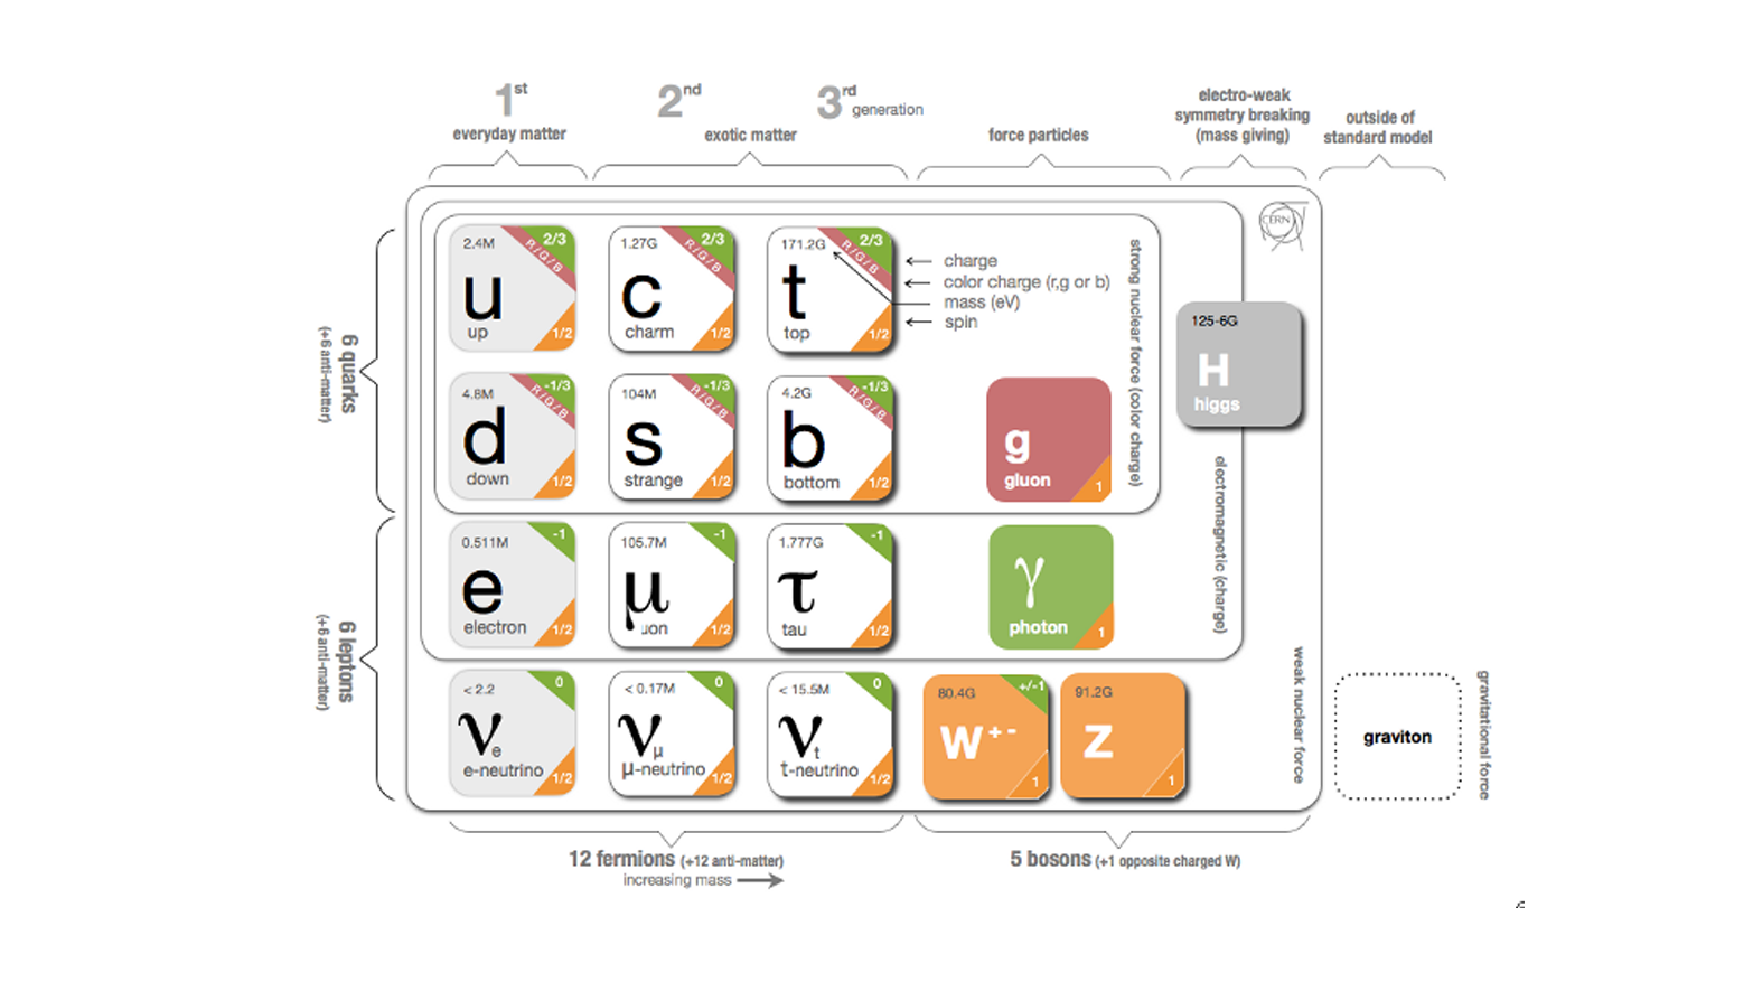
\includegraphics[width = \textwidth]{figures/standardmodel_galbraith_carsten.pdf}
    \caption{Schematic diagram of all elementary particles in the SM.  Particles are grouped according to their properties and the forces through which they interact with other particles~\cite{galbraith_ux_2013}.}
    \label{fig:standard_model}
\end{figure}

The known elementary particles described by the SM are represented in Figure~\ref{fig:standard_model}.  There are 12 matter particles (six quarks and six leptons), 4 force-mediating particles, and the Higgs boson. Each matter particle has a corresponding anti-matter particle with the same mass but opposite charge, not represented in Figure~\ref{fig:standard_model}. The different forces of nature are understood to be the result of the exchange of force-mediating particles between interacting (coupled) particles. Photons are mediators of the electromagnetic force, W+/- and Z bosons are mediators of the weak force, and gluons are mediators of the strong force\iffalse[GRIFFITHS]\fi. At high energy, the SM describes the electromagnetic and weak forces as stemming from a unified electroweak force\iffalse[PESKIN]\fi. The Higgs boson field interacts with the particles mediating the unified electroweak force to distinguish the weak and electromagnetic forces from each other at lower energies and give particles (except neutrinos) a mass. This is called electroweak symmetry breaking\iffalse[PESKIN]\fi. 

Quarks are matter particles that are sensitive to all forces; notably they are the only matter particles sensitive to the strong force\iffalse[GRIFFITHS]\fi. Protons and neutrons are made up of quarks and gluons, and the strong force is responsible for their existence and mutual attraction into nuclei~\cite{bertulani_nuclear_2007}. Leptons are particles not sensitive to the strong force. Charged leptons include the electron, which once part of atoms is responsible for chemistry. Of particular importance for this thesis is the charged lepton called a muon. It is like the electron but its mass is $\sim$200 times larger than that of the electron. Muons have a lifetime of \SI{2.2}{\micro\second}~\cite{zyla_review_2020} and decay predominantly as $\mu \rightarrow e^{-}\overline{\nu}_{e}\nu_{\mu}$ .Neutrinos are neutral, almost massless leptons that only interact through the weak force\iffalse[GRIFFITHS]\fi. 

Common matter is made up of the lightest constituents of the SM: up and down quarks, electrons and photons. The other particles are produced in high-energy environments but then decay to the lightest constituents. Such high energy environments include the conditions present in the early universe~\cite{carroll_introduction_2007}, astrophysical sources, and particle accelerators\iffalse[REV PART PHYS, GRIFFITHS]\fi. The presence of the particles of the SM at the beginning of the universe means that their interactions and decays are fundamental for the study of the evolution of the early universe~\cite{carroll_introduction_2007}. Many high energy astrophysical sources, like supernovae, generate particles that rain down on Earth as cosmic rays~\cite{boezio_chemical_2012}\iffalse[BOEZIO, REV PART PHYS, GRIFFITHS]\fi. Particle accelerators have been built to create controlled environments of high-rate, high-energy particle collisions at high energy where the production and decay of elementary particles can be directly studied\iffalse[GRIFFITHS, REV PART PHYS]\fi.

% --------------------------------------------------
\section{Beyond the Standard Model}
% --------------------------------------------------

Despite its success at describing most experimental observations to date, there is ample evidence that the SM is not a complete description of natural phenomena at the smallest scales. For example, the SM has a large number of free parameters, the values of which have to be fine-tuned to fit experimental observations. This is part of the so-called ``naturalness'' problem.

Furthermore, the SM provides no explanation for several open questions in particle physics. First, neutrinos in the SM are assumed to be massless and do not gain mass in the same way as the other particles. However, neutrinos were confirmed to change between their different flavours ($\nu_e$, $\nu_\mu$, $\nu_\tau$) in 2013~\cite{aharmim_combined_2013}, which can only occur if neutrinos do have mass~\cite{pontecorvo_neutrino_1967}. The neutrino mass requires physics beyond the Standard Model~\cite{bilenky_massive_1987}. Second, several astrophysical and cosmological measurements suggest the presence of ``dark matter'' making up 85~\% of the matter content of the universe~\cite{young_survey_2017}. The nature of dark matter is unknown and so far there is no SM explanation~\cite{munoz_dark_2004}. Third, the SM does not explain the origin and nature of the matter-antimatter asymmetry that produced our matter-dominated universe. Finally, the SM does not include a description of gravity.

Theoretical extensions beyond the Standard Model (BSM) aim to address some of these questions, often predicting existence of yet-unseen elementary particles or physics phenomena beyond those predicted by the SM. These hypothetical new physics phenomena or new particles can be searched for at particle accelerators. 
%For example, super-symmetry (SUSY) predicts that each SM particle has a heavier super-symmetric partner. SUSY would explain the origin of dark matter with weakly interacting massive particles, would solve the so-called ``naturalness'' problem in the SM~\cite{jungman_supersymmetric_1996}. 

% --------------------------------------------------
\section{Studying high energy particle physics with accelerators}
% --------------------------------------------------

In particular, particle accelerators of increasingly higher energy have a long history of enabling the discovery of predicted particles. These include, for example, the discovery of the W~\cite{arnison_W_1983, banner_observation_1983} and Z bosons~\cite{arnison_Z_1983, bagnaia_evidence_1983}, the top quark~\cite{cdf_collaboration_observation_1995, d0_collaboration_observation_1995}, and most recently, the Higgs boson~\cite{the_atlas_collaboration_observation_2012, the_cms_collaboration_observation_2012}. The discovery of the Higgs boson marked the completion of the SM as it is known today.

Based on the established success of the SM, there are two approaches to particle physics research. One approach is to search for the existence of new physics phenomena predicted to exist in BSM theories and the other is to test the validity of the SM to a high degree of accuracy to search for flaws in the model. Standard Model predictions are generally expressed in terms of the probability of a specific physics process to occur, expressed as a cross section in units of barns (with 1 barn $=$ 10$^{-28}$ m$^{2}$).  As an example, Figure~\ref{fig:standard_model} shows a summary of cross section measured for different physics processes using the ATLAS experiment and their comparison with the predictions of the SM. Most cross section measurements agree well within one standard deviation with the SM predictions. 

\begin{figure}
    \centering
    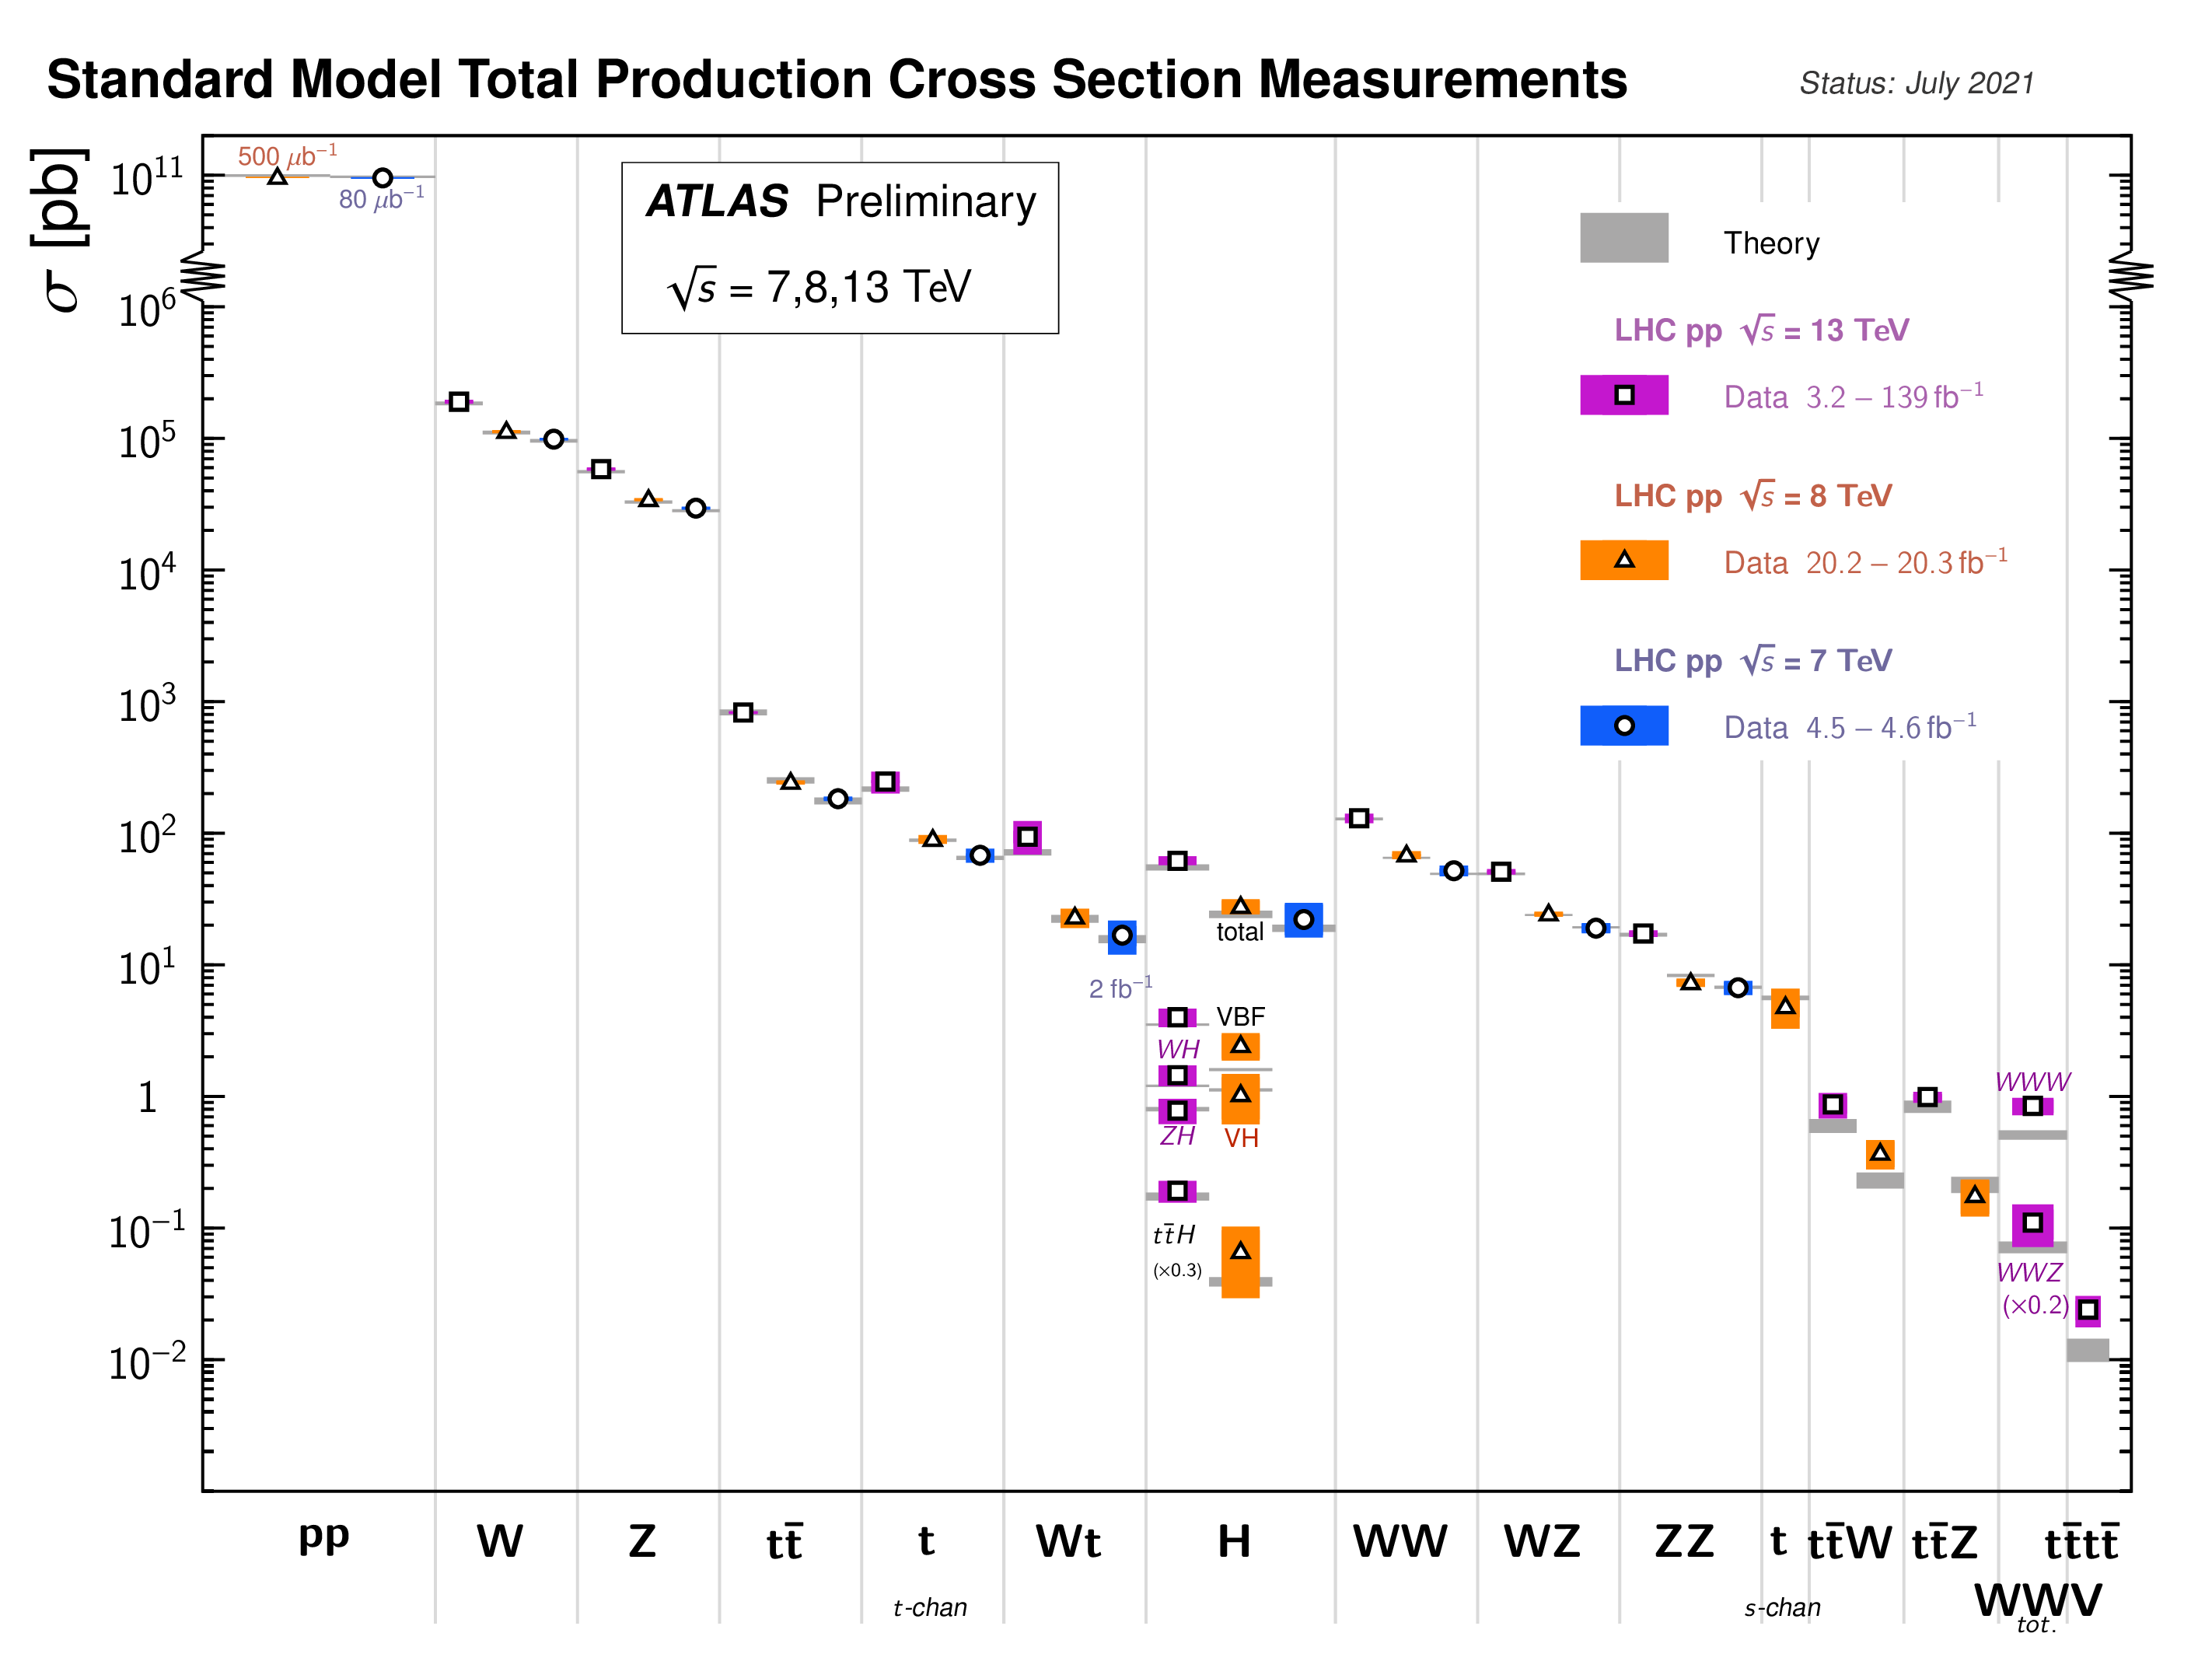
\includegraphics[width = \textwidth]{figures/atlas_cross_sections.png}
    \caption{Production cross sections of different final states measured by the ATLAS experiment at the LHC. Comparison with the SM theory predictions is also shown~\cite{atlas_public_web_sm}.}
    \label{fig:atlas_cross_sections}
\end{figure}

Particle accelerators provide a controlled and high-collision rate environment that makes them ideal places to search for new physics phenomena and to carry out systematic tests of the SM. The LHC is the highest energy collider in the world so it can access physics that no other accelerator can. A description of the LHC and the ATLAS detector are provided in the next chapter. 

% ==================================================
% CHAPTER 3: The LHC and the ATLAS experiment %
% ==================================================

\chapter{The LHC and the ATLAS experiment}
\label{chap:lhc_atlas}

The Large Hadron Collider (LHC) is the world's most energetic particle accelerator and the ATLAS experiment is used to record the results of particle collisions at the LHC. In this chapter, details about both that are necessary to understand the High-Luminosity LHC upgrade project and the ATLAS experiment NSW upgrade are presented.

% --------------------------------------------------
\section{The Large Hadron Collider}
% --------------------------------------------------

% Include order for inst lum.
% Include bunch crossing frequency
The LHC is an accelerator \SI{27}{\kilo\meter} in circumference and located $\sim$\SI{100}{\meter} underground at the CERN laboratory near Geneva, Switzerland~\cite{evans_lhc_2008}. It has two beam pipes within which bunches of protons counter-circulate before being collided in the center of one of four major experiments, such as the ATLAS experiment (discussed in section~\ref{sec:atlas}). Protons are guided on the circular trajectory using 1232 superconducting dipole magnets capable of a maximum field of \SI{8.33}{T}. Radio-frequency accelerating cavities are used to accelerate protons to a the maximum design energy of 7 TeV~\cite{bruning_lhc_2004}.  During LHC Run-1 (2011-2012), protons were collided at a collision center-of-mass energy of 7 TeV and 8 TeV~\cite{atlas_luminosity_run1}. During LHC Run-2 (2015-2018), the center-of-mass energy of proton collisions was increased to 13 TeV~\cite{atlas_luminosity_run2}, close to the maximum design value of 14 TeV~\cite{bruning_lhc_2004}. It is not actually the protons that interact, but the constituent quarks and gluons that each carry some fraction of the energy and momentum of the collisions.

% There are two main branches of study that can be pursued with the LHC and ATLAS. First, properties predicted by the standard model (SM) of particle physics can be measured. Else, physicists can search for evidence of processes predicted by theories beyond the standard model. Both the SM measurement and search analyses are based on measuring the number of times a given process occurs and comparing it to expectations. In this way, the number of proton-proton interactions created by the LHC directly affects the statistics available to do SM measurements and searches using the ATLAS experiment.

\paragraph*{Luminosity} \hfill \break
The number of proton-proton interactions generated by the LHC directly affects the statistics available to make measurements of interaction cross sections.
%IF YOU DON'T NEED TO DEFINE LUMINOSITY
% The number of interactions is quantified by luminosity, a property of the accelerator and its operating conditions~\cite{zyla_review_2020}. When the instantaneous luminosity is integrated over a data collection period and multiplied by the cross section of a given process, the result is the expected number of times that process occurs (so luminosity has units of inverse cross section). Since luminosity is derived from the accelerator parameters, it is the link between the machine and the statistical power of potential measurements. 
% IF YOU NEED TO DEFINE LUMINOSITY
% THIS SECTION IS NOT CITED, probably cite wiht zyla_review_2020
Predicting the number of proton-proton interactions requires defining a metric called luminosity~\cite{zyla_review_2020}. The luminosity of a particle collider is the number of particles an accelerator can send through a given area per unit time. It is calculated from the measurable quantities in Equation~\ref{eqn:inst_lum}:

\begin{equation}
\mathcal{L} = \frac{f N_{1} N_{2} }{4 \pi \sigma_{x} \sigma_{y}}~,
\label{eqn:inst_lum}
\end{equation}

where $f$ is the frequency of the bunch crossings (\SI{25}{\nano\second}), $N_{1}$ and $N_{2}$ are the number of protons in each bunch ($\sim 10^{11}$ protons / bunch), and $\sigma_{x}$ and $\sigma_{y}$ are the RMS of the spatial distributions of the bunch. Therefore, luminosity is a property of accelerator beams, which are set by the capabilities of the accelerator. The design luminosity of the LHC was $10^{34}$ cm$^{-2}$s$^{-1}$. The units of luminosity are an inverse area; multiplying the luminosity by the cross section of a given process gives the expected rate for that process.

Integrating the \textit{instantaneous} luminosity (equation~\ref{eqn:inst_lum}) over a period of data collection time gives the integrated luminosity,

\begin{equation}
L = \int \mathcal{L} \left( t \right) \,dt
\label{eqn:int_lum}
\end{equation}

which is related to the total number of interactions. In this way, the luminosity is the link between the accelerator and the statistical power of measurements to be made with the data collected. So far, the LHC provided an integrated luminosity of \SI{28.26}{\per\femto\barn} in Run-1~\cite{atlas_luminosity_run1} and \SI{156}{\per\femto\barn} in Run-2~\cite{atlas_luminosity_run2}.

% --------------------------------------------------
\section{The High-luminosity LHC}
% --------------------------------------------------
At the end of the LHC program in 2025, the statistical gain on measurements in running the LHC further will become marginal. The High-Luminosity LHC (HL-LHC)~\cite{hl_lhc_tdr} project consists of the upgrade of the LHC infrastructure to achieve a nearly ten fold increase in instantaneous luminosity, thereby improving measurement statistics as well. Also, some systems will need repair and replacement to operate past $\sim$2020. The LHC will continue to be the most energetic accelerator in the world for years to come and is the only accelerator capable of directly producing the Higgs boson and top quarks. Therefore, the European Strategy for Particle Physics made it a priority ``to fully exploit the physics potential of the LHC'' with ``a major luminosity upgrade''~\cite{european_strategy_for_particle_physics}. The goal is for the HL-LHC to provide an integrated luminosity of \SI{3000}{\per\femto\barn} in the 12 years following the upgrade. The luminosity actually achieved will depend on a combination of technological advances and upgrades in progress that affect the factors contributing to luminosity defined in equation~\ref{eqn:inst_lum}~\cite{hl_lhc_tdr}. Figure~\ref{fig:hl-lhc} shows the projected schedule of the HL-LHC upgrades and operation~\cite{hl-lhc_plan_picture_website}.

\begin{figure}
    \centering
    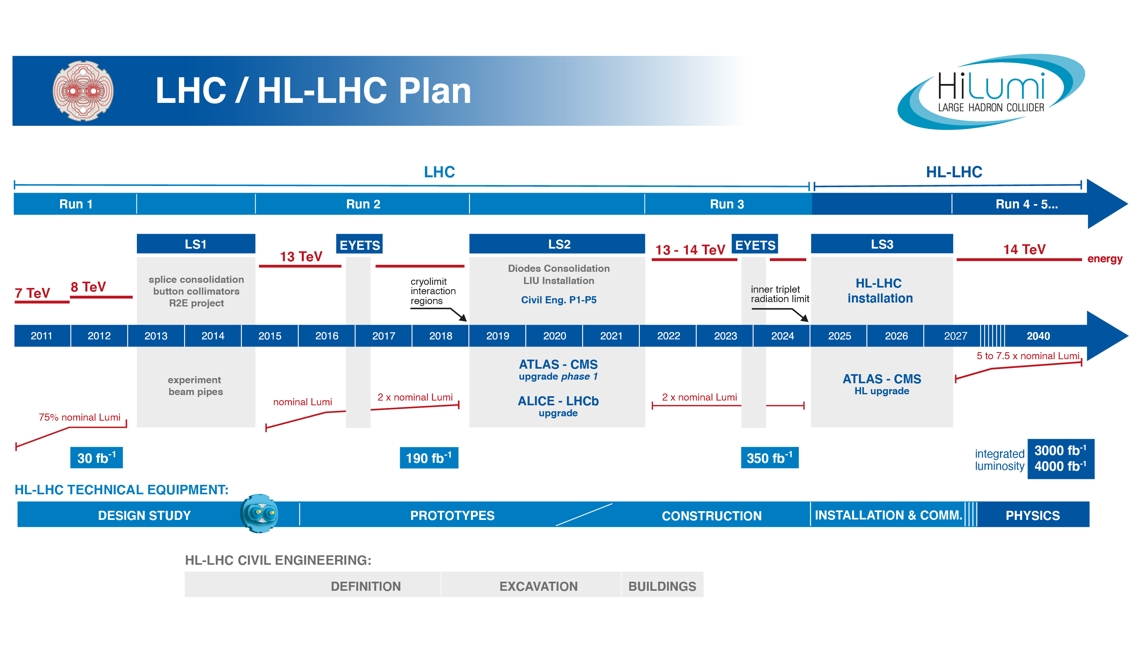
\includegraphics[width = \textwidth]{figures/HL-LHC-updated-January-2021_small.jpg}
    \caption{The LHC/HL-LHC timeline~\cite{hl-lhc_plan_picture_website}. The integrated luminosities collected and projected for each run of the LHC are shown in blue boxes below the timeline and the center of mass energy of the collisions is shown in red above the timeline. The top blue arrow labels the run number. The acronym ``LS'' stands for ``long shutdown'' and indicates periods where the accelerator is not operating. During the shutdowns, upgrades to the LHC and the experiments are taking place. This timeline was last updated in January, 2021, and reflects changes in the schedule due to the ongoing pandemic. }
    \label{fig:hl-lhc}
\end{figure}

% The increase in statistics the HL-LHC will improve measurements of standard model parameters and improve searches for unobserved phenomena~\cite{dainese_physics_2018}. A particular measurement that will benefit from the increased statistics is of the triple-Higgs coupling. Measuring the coupling measures the shape of the Higgs potential responsible for electroweak symmetry breaking. Any discrepancy with the SM prediction will show that there must be other sources of electroweak symmetry breaking~-- if there is such another source, it could be an avenue to study the other questions the SM does not address. Also, the sensitivity to several exotic Higgs decays to BSM particles will be improved. Many of the products of exotic Higgs decays are dark matter candidates or otherwise could extend the scope of the SM.

% Higgs couplings to particles will all be measured to the percent level at the HL-LHC and sensitivity to SM predicted Higgs decays will increase. Also, the sensitivity to several exotic Higgs decays to BSM particles will be improved. Many of the products of exotic Higgs decays are dark matter candidates or otherwise could extend the scope of the SM. The LHC is the only accelerator energetic enough to directly produce Higgs bosons, so it is the only tool able to probe questions about the Higgs.

One of the most anticipated measurements at the HL-LHC is the value of the triple-Higgs coupling. Measuring the coupling will allow the determination of the shape of the Higgs potential responsible for electroweak symmetry breaking. Any discrepancy with respect to the SM prediction will show that there must be other sources of electroweak symmetry breaking, and hence physics phenomena beyond the SM. The LHC is the only accelerator where the Higgs can be produced directly. The HL-LHC upgrade is required to produce a significant sample of Higgs produced in pairs to make a statistically meaningful measurement~\cite{dainese_physics_2018, cepeda_report_2018}. Accordingly, detector sensitivity to various Higgs decays will be important at the HL-LHC.
%The estimated number of interactions of a given type per bunch crossing is given by equation~\ref{eqn:num_interactions}.
%\begin{equation}
%\mu = \sigma \delta t\mathcal{L}
%\label{eqn:num_interactions}
%\end{equation}

% The energies accessible by the accelerator make it unique infrastructure with which to study processes of the standard model of particle physics and search for new phenomenon beyond the standard
% model. Considerable progress has been made towards answering the questions originally used to motivate the construction of the LHC, but many remain unanswered or only partially answered~ \cite{brianti_large_1984}. Therefore, the continued use and maintenance of the accelerator 

% --------------------------------------------------
\section{The ATLAS experiment}
% --------------------------------------------------
\label{sec:atlas}

The ATLAS experiment~\cite{collaboration_atlas_2008} was designed to support all the physics goals of the LHC. It is \SI{44}{\meter} long and \SI{25}{\meter} in diameter, and weighs 7000 tonnes. The ATLAS experiment is centered around one of the LHC's interaction points (a place where the beams collide). As shown schematically in figure~\ref{fig:atlas}, ATLAS consists of an array of particle detector subsystems arranged concentrically around the beam pipe.  The ATLAS experiment is cylindrical because it aims to provide 4$\pi$ coverage around the interaction point. In reference to the cylindrical geometry of the experiment, it is helpful to separate the subsystems of ATLAS into the so-called ``barrel'' and ``endcap''/``forward'' regions.

\begin{figure}
    \centering
    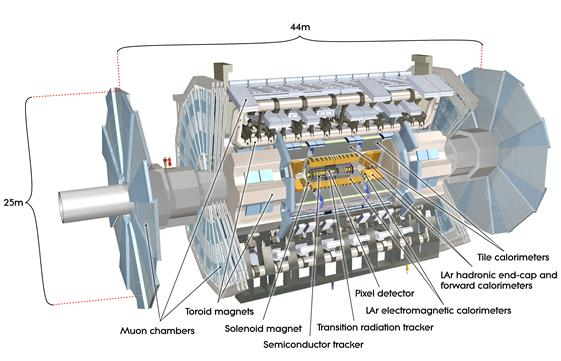
\includegraphics[width = \textwidth]{figures/atlas_diagram.png}
    \caption{Diagram of the ATLAS experiment, with the various detector subsystems labelled~\cite{collaboration_atlas_2008}.}
    \label{fig:atlas}
\end{figure}

For analysis purposes, a spherical coordinate system is defined. The azimuthal angle $\phi$ is measured around the beampipe and the polar angle $\theta$ is measured from the beam pipe. The polar angle is more often expressed in terms of pseudo-rapidity, defined as $\eta = -\ln\tan\left(\theta/2\right)$.  Pseudo-rapidity values vary from 0 (perpendicular to the beam) to $\pm\infty$ (parallel to the beam, defined as the z-direction). Pseudo-rapidity is an approximation to the rapidity of a particle when its momentum is much greater than its mass. It is useful to describe the direction of outgoing particles in proton-proton collisions because differences in rapidity are invariant to a Lorentz boost along the beam direction.

The ATLAS experiment provides identification and kinematic measurements for each particle created after the initial collision by assembling offline the information recorded by each subsystem of ATLAS. With this information, signatures of processes of interest can be identified and studied. An overview of the main ATLAS subsystems is given below.

%TODO : CITE TRANS RAD
\paragraph*{The inner detector} \hfill \break
The inner detector~\cite{atlas_inner_detector_tdr_1, atlas_inner_detector_tdr_2} (figure~\ref{fig:atlas_inner_detector}) is for precise measurements of charged particle trajectories, measurement of primary and secondary interaction vertices and to assist in the identification of electrons. A \SI{2}{\tesla} solenoid with field parallel to the beam bends the trajectory of outgoing charged particles. A measurement of the bending radius of each charged particle provides information about its momentum. The innermost part of the inner tracker is made of high-resolution semiconductor pixel and strip detectors while the outermost part is made of straw-tubes. The straw tubes are used in the trajectory measurements but they are also interspersed with material designed to enhance the creation of transition radiation. Transition radiation occurs when a highly relativistic charged particle traverses a material boundary. The amount of transition radiation emitted by a charged particle is detected by the straw-tubes and is used to identify electrons. 

 that generate and detect transition radiation

\begin{figure}
    \centering
    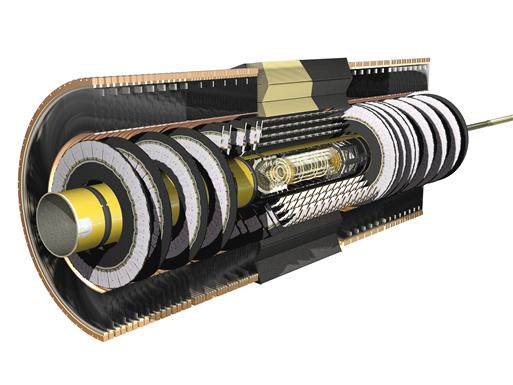
\includegraphics[width = 0.5\textwidth]{figures/atlas_inner_detector.jpg}
    \caption{Schematic diagram of the ATLAS experiment's inner detector, with the different segments and the technology used labelled~\cite{collaboration_atlas_2008}.}
    \label{fig:atlas_inner_detector}
\end{figure}

% YOU ARE HERE
\paragraph*{Calorimetry system} \hfill \break
Electromagnetic and hadronic sampling calorimeter units are used to record the energy of electrons, photons and jets. A combination of liquid-argon (LAr) electromagnetic and hadronic calorimeters~\cite{atlas_lar_cal_tdr} and tile-scintillator hadronic calorimeters~\cite{atlas_tile_cal_tdr} cover the rapidity range $|\eta| < 4.9$, as shown in figure~\ref{fig:atlas_calorimeter}.

\begin{figure}
    \centering
    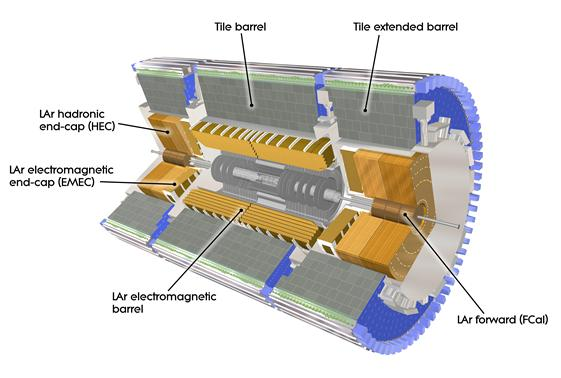
\includegraphics[width = 0.5\textwidth]{figures/atlas_calorimeter.png}
    \caption{Diagram of the ATLAS calorimeter system, with the different segments and the technology used labelled~\cite{collaboration_atlas_2008}.}
    \label{fig:atlas_calorimeter}
\end{figure}

The calorimeters cause incoming charged particles to shower and deposit their energy in the sensitive volume. Only muons and neutrinos are known to pass the calorimeters to the muon spectrometer.  Particles other than those mentioned would have decayed in the inner detector before reaching the calorimeter. 

\paragraph*{Trigger system} \hfill \break
It would be impossible to record all the data from bunch crossings every \SI{25}{\nano\second}, corresponding to a rate of $\sim$\SI{40}{MHz}. ATLAS has a multi-level trigger system to select events of interest for permanent storage. The Level-1 (L1) hardware trigger~\cite{atlas_l1_trigger_tdr} uses partial-granularity information from the muon spectrometer and calorimeter to trigger on high $p_T$ muons, electrons, jets, high missing transverse energy, and $\tau$ decaying to hadrons. The maximum L1 trigger rate ATLAS can accommodate is \SI{100}{kHz} with a latency of \SI{2.5}{\micro\second}. After Run-3 an upgrade of the trigger system will allow for a higher rate and more latency, but for now these are the working limits~\cite{tdaq_phase2_tdr}.

% The Level-1 (L1) hardware trigger uses the muon spectrometer's TGCs and RPCs to trigger on high $p_T$ muons and the calorimeter detector units to trigger on electrons, jets, high missing transverse energy, and $\tau$ decaying to hadrons, with a maximum trigger rate of \SI{100}{kHz} and latency of \SI{2.5}{\micro\second}. The L1 trigger only uses a fraction of the granularity offered by the detectors.

The L1 trigger is used to define regions of interest that are fed into the software high level trigger (HLT), in which the full granularity of the muon spectrometer and calorimeter are used with information from the inner detector to reduce the trigger rate to 1 kHz. Events that pass the L1 and HLT trigger are recorded for use in offline analysis~\cite{atlas_hlt_trigger_tdr}.

The ATLAS trigger system is described in the references above but the trigger rates quoted here are after the upgrades implemented for Run-2, described in~\cite{martinez_run-2_2016}.

\paragraph*{Muon spectrometer} \hfill \break
The muon spectrometer has multiple layers, each of which records the position of a passing muon. Magnetic deflection by superconducting air-core toroid magnets bend the muon tracks. The position information recorded in each layer and the magnetic field are used to reconstruct each muon's momentum. In the barrel of ATLAS, eight coils bent into ``racetracks'' arranged around the beampipe provide the magentic field. In the forward region, two end-cap toroids each with eight smaller racetrack-shaped coils arranged symmetrically around the beampipe are inserted in the ends of the barrel toroid~\cite{atlas_magnet_tdr}. Figure~\ref{fig:atlas_muon_spectrometer} shows the toroid magnets and the different parts of the ATLAS muon spectrometer~\cite{collaboration_atlas_2008}.

\begin{figure}
\centering
\begin{subfigure}{.5\textwidth}
  \centering
  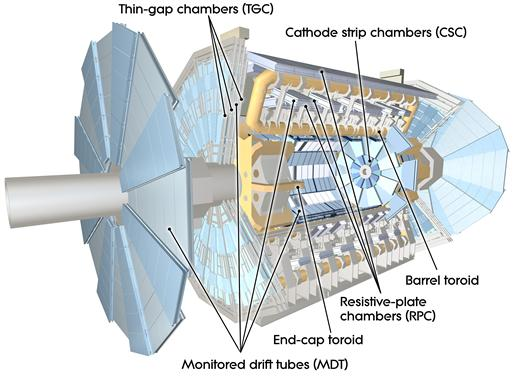
\includegraphics[width=\linewidth]{figures/atlas_muon_spectrometer.jpg}
  \caption{}
  \label{fig:atlas_muon_spectrometer_3D}
\end{subfigure}%
\begin{subfigure}{.5\textwidth}
  \centering
  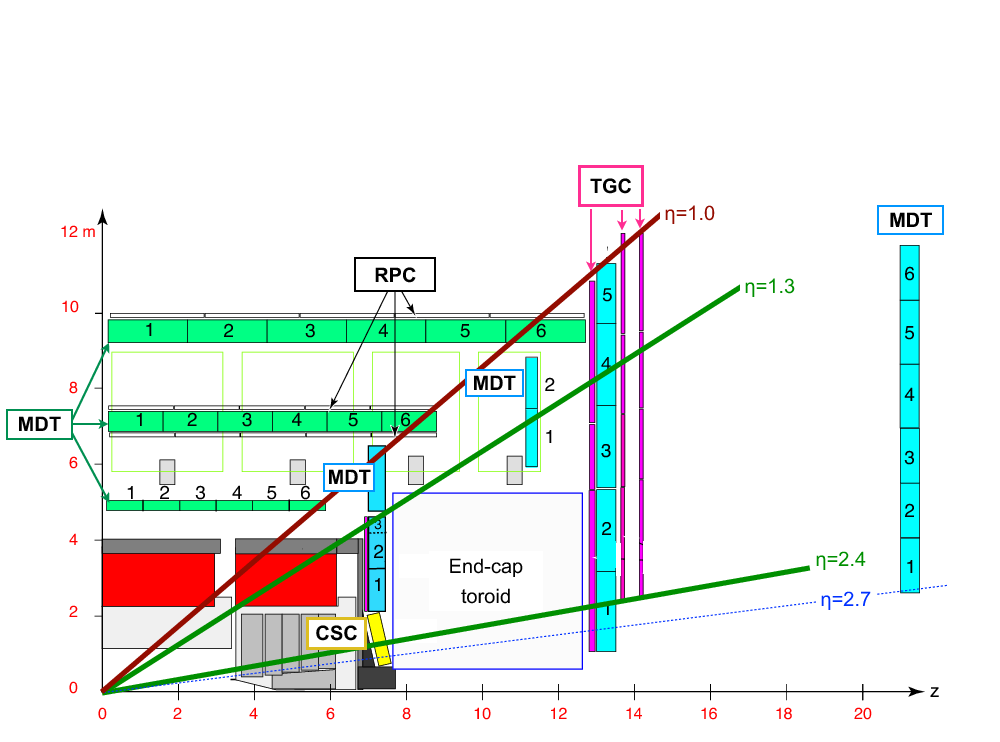
\includegraphics[width=\linewidth]{figures/atlas_old_muon_spec_quarter_cut_recolour.png}
  \caption{}
  \label{fig:atlas_muon_spectrometer_cut}
\end{subfigure}
\caption{(a) The ATLAS muon spectrometer~\cite{collaboration_atlas_2008}. (b) A quarter-cut of ATLAS, with the interaction point in the bottom left corner. The small wheel is just left of the end cap toroid, the big wheel is to its right, and the outer wheel is the rightmost structure~\cite{atlas_performance_muon_trigger_2015}.}
\label{fig:atlas_muon_spectrometer}
\end{figure}

The muon spectrometer~\cite{atlas_muon_spectrometer_tdr} is separated into detectors used for precision offline tracking and for triggering. Three layers of monitored drift tubes (MDTs) or cathode strip chambers (CSCs) are used for tracking. The position of the muon track in each of the three layers allows reconstruction of the track and hence momentum. For the design momentum resolution of $\Delta p_T / p_T <$~1$\times$10$^{-4}~p$~/~GeV for $p_T <$~300~GeV and a few percent for lower $p_T$ muons, the MDTs and CSCs required position resolution of \SI{50}{\micro\meter} each. Accordingly, an optical alignment system was designed to monitor and correct for chamber positions~\cite{atlas_muon_spectrometer_tdr, aefsky_optical_2008}. 

% Precision tracking is done offline for events passing the muon trigger. Each of the barrel and encap systems have three layers of MDTs that record the position of the muon as it passes through each layer. Knowing the magentic field, the muon's momentum can be extracted. For the design momentum resolution of $\Delta p_T / p_T <$ 1$\times$10$^{-4}~p$ / GeV for $p_T < 300 GeV$ and a few percent for lower $p_T$ muons, the MDTs and CSCs required position resolution of \SI{50}{\micro\meter} each. Accordingly, an optical alignment system was designed to monitor and correct for chamber positions~\cite{atlas_muon_spectrometer_tdr, aefsky_optical_2008}. 

% ON MUON TRIGGERING IN THE ENDCAP
% Decide how you want to do this based on the next section.
% At least 2 TGC layers in coincidence comes from muon spectrometer TDR; coincidence with "forward inner" detectors (small wheel) comes from Run-2 trigger upgrades paper, Martinez.
% NSW TDR says there are TGC layers in the small wheel that are the forward inner detectors added to Run-2 triggering.
% \textcolor{red}{The Run-2 L1 muon trigger was passed if TGC layers (two for low $p_T$ muons, three for high $p_T$ muons) of the big wheel fired in coincidence with a hit from the MDTs of the small wheel on the order of the bunch crossing time. The regions of interest defined by the TGCs were fed into the HLT, where MDT and TGC data could be combined for further cuts. The $p_T$ resolution of the L1 trigger is improved by the MDT tracking information. \textit{I'll decide how I want to do this after writing the motivation for the NSW}}
Resistive plate chambers (RPCs) are used for triggering in the barrel and thin-gap chambers (TGCs) are used for triggering in the endcaps. The positions of each type of chamber are sketched in figure~\ref{fig:atlas_muon_spectrometer_cut}. Often, the endcap muon spectrometer is separated into three wheels~-- the small wheel, big wheel, and outer wheel~-- ordered by proximity to the interaction point. In Run-1, low (high) $p_T$ muons were triggered on at L1 if two (three) of the RPCs or TGCs layers around the big wheel fired in coincidence, for the barrel and endcaps respectively~\cite{atlas_l1_trigger_tdr}. After Run-1 it was discovered that up to 90\% of the triggers in the endcap were fake, caused by background particles generated in the material between the small wheel and the big wheel~\cite{nsw_tdr}.  To reduce the fake rate in Run-2, the TGCs on the inside of the small wheel also had to register a hit. The added condition reduced the trigger rate by 50\% in the range 1.3 $< |\eta| <$ 1.9~\cite{martinez_run-2_2016}. The effectiveness of the solution was limited since the $|\eta|$-range of the small wheel TGCs was limited to 1.0 $< |\eta| <$ 1.9 and the position resolution of the small wheel TGCs is coarse~\cite{nsw_tdr}.

% In the barrel, three layers of MDTs are used for precision tracking, and resistive plate chambers (RPCs) are used for triggering. The endcaps of the muon spectrometer are composed of three wheels each, the small wheel (SW), big wheel, and outer wheel. All three wheels use MDTs for precision offline tracking, but cathode strip chambers (CSCs) are used in the forward region of the small wheel because they can better handle the increased background. Thin gap  chambers

% The big wheel and the outer wheel have MDTs for offline precision tracking and the thin gap chambers (TGCs) on either side for triggering. In the first two runs of ATLAS, offline precision tracking on the small wheel was done with MDTs and cathode strip chambers (CSCs), and their output did not contribute to the trigger.~\cite{atlas_muon_spectrometer_tdr}. 

% Sentences if you go without 1/4 cut figure
% In the barrel, three layers of monitored drift tubes (MDTs) are arranged between, above and below the barrel toroid magnets. They are used for precision tracking. On both sides of the middle layer of  MDTs and on the top of the top layer of MDTs are resitive plate chambers (RPCs), used for triggering.
%  The inner part had cathode strip chambers (CSCs), which had higher granularity to handle the increased background radiation rate in the forward region

% The muon spectrometer is the outermost layer of the ATLAS detector, since only muons (and neutrinos) can pass through the calorimeters. For muons that are ejected towards the end-caps of ATLAS, their trajectory is bent by the magentic field and their position recorded by three successive wheels of muon detectors. With each wheel providing the position of the muon along its trajectory and knowledge of the magentic field, the momentum of the muon generated in the collision can be reconstructed. 
% ==================================================
% CHAPTER 4: The New Small Wheels %
% ==================================================

\chapter{The New Small Wheels}
\label{chap:nsw}
% Edit count: Lia - 0, Brigitte - 0

% --------------------------------------------------
\section{Motivation for the New Small Wheels}
% --------------------------------------------------

The hit rate of all detector systems will significantly increase during HL-LHC operation because of the increase in luminosity. The increased rate presents a challenge for both the tracking and triggering capabilities of the muon spectrometer~\cite{nsw_tdr}.

In terms of precision tracking, the maximum hit rate in the MDTs is expected to reach above 300 kHz by the end LHC operation.  At this rate, the hit efficiency of MDTs decreases by 35\%, mostly due to the long dead-time of the chambers. Losing hits in the small wheel will reduce the high $p_T$ muon momentum resolution. The decrease in resolution will affect the ability to search for, for example, the decay of hypothetical heavy bosons (W', Z') or other hypothetical particles beyond the SM~\cite{dainese_physics_2018}.

Already during LHC Run-2 operation, the forward muon trigger system had to cope with a very high fake rate, even with the inclusion of TGC data from the small wheel as part of the trigger criteria.  At the luminosity expected in Run-3, it is estimated that 60 kHz out of the maximum L1 trigger bandwidth of 100 kHz would be taken up by forward muon triggers. To address this challenge, a possible solution would be to raise the minimum $p_T$ threshold from \SI{20}{\giga\electronvolt} to \SI{40}{\giga\electronvolt}. However, this would have an adverse impact on the ability to study several physics processes of interest that depend on low $p_T$ muons, particularly the Higgs decay to two muons, the Higgs decay to two tau leptons and hypothetical particle decays beyond the SM~\cite{nsw_tdr}.

The NSWs will address both of these problems. They will be made of precision tracking chambers suitable for the expected hit rates during the HL-LHC and triggering chambers capable of \SI{1}{mrad} track angular resolution. The idea behind the design triggering capability of the chambers is to allow matching of track segments measured by the NSW with track segments from the big wheel to discard tracks not originating from the interaction point. Figure~\ref{fig:nsw_track_triggering} illustrates this point: the Run-2 trigger system would have triggered on all three tracks (A, B, C) while with the NSW the trigger system would only trigger on track A. The NSWs will therefore make it possible to maintain a low muon $p_T$ trigger threshold and maintain an adequate muon momentum resolution during HL-LHC operations, which will allow the full exploitation of the physics potential of this research program~\cite{nsw_tdr}.

\begin{figure}
    \centering
    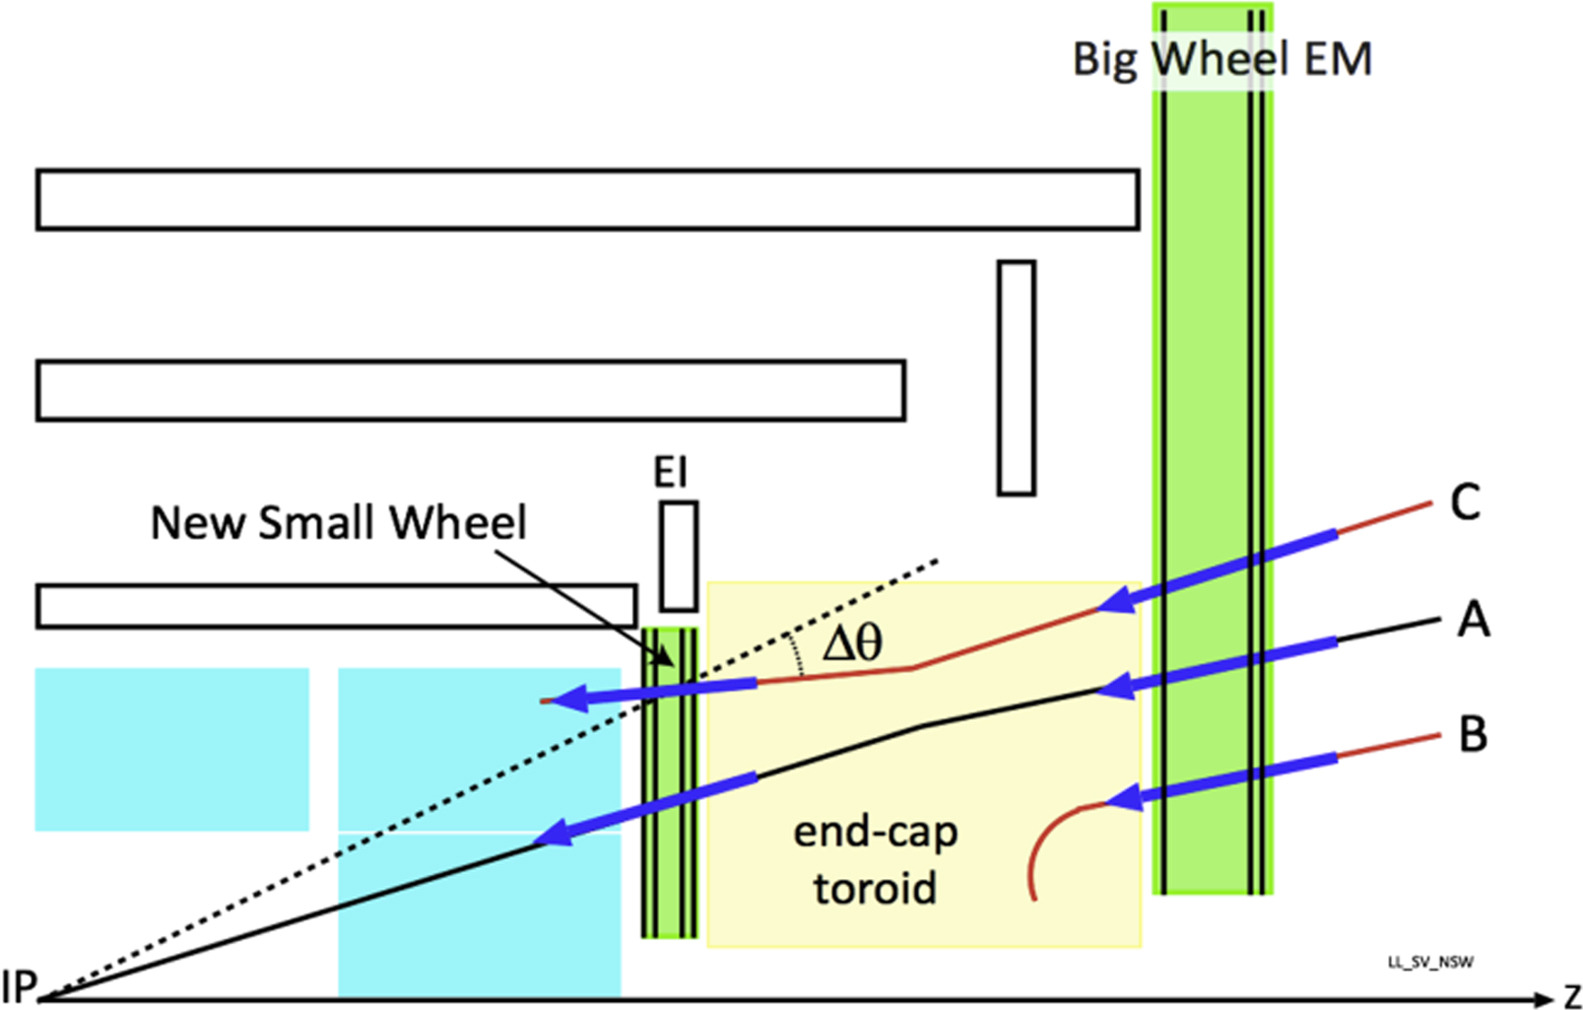
\includegraphics[width = 0.9\textwidth]{figures/perez-codina_NSW_tracks.jpg}
    \caption{A schematic diagram of a quarter cross section of the ATLAS muon spectrometer, with the interaction point (IP) in the bottom left corner. Three possible tracks are labeled. Ideally, track A would be triggered on while track B and C discarded. With the old small wheel, all three tracks would be recorded. With the NSW, only track A would be recorded~\cite{nsw_tdr}.}
    \label{fig:nsw_track_triggering}
\end{figure}

\newpage
\thispagestyle{empty}
\newgeometry{top=0.5in,bottom=0.5in}
\begin{figure}
\centering
\begin{subfigure}{\textwidth}
  \centering
  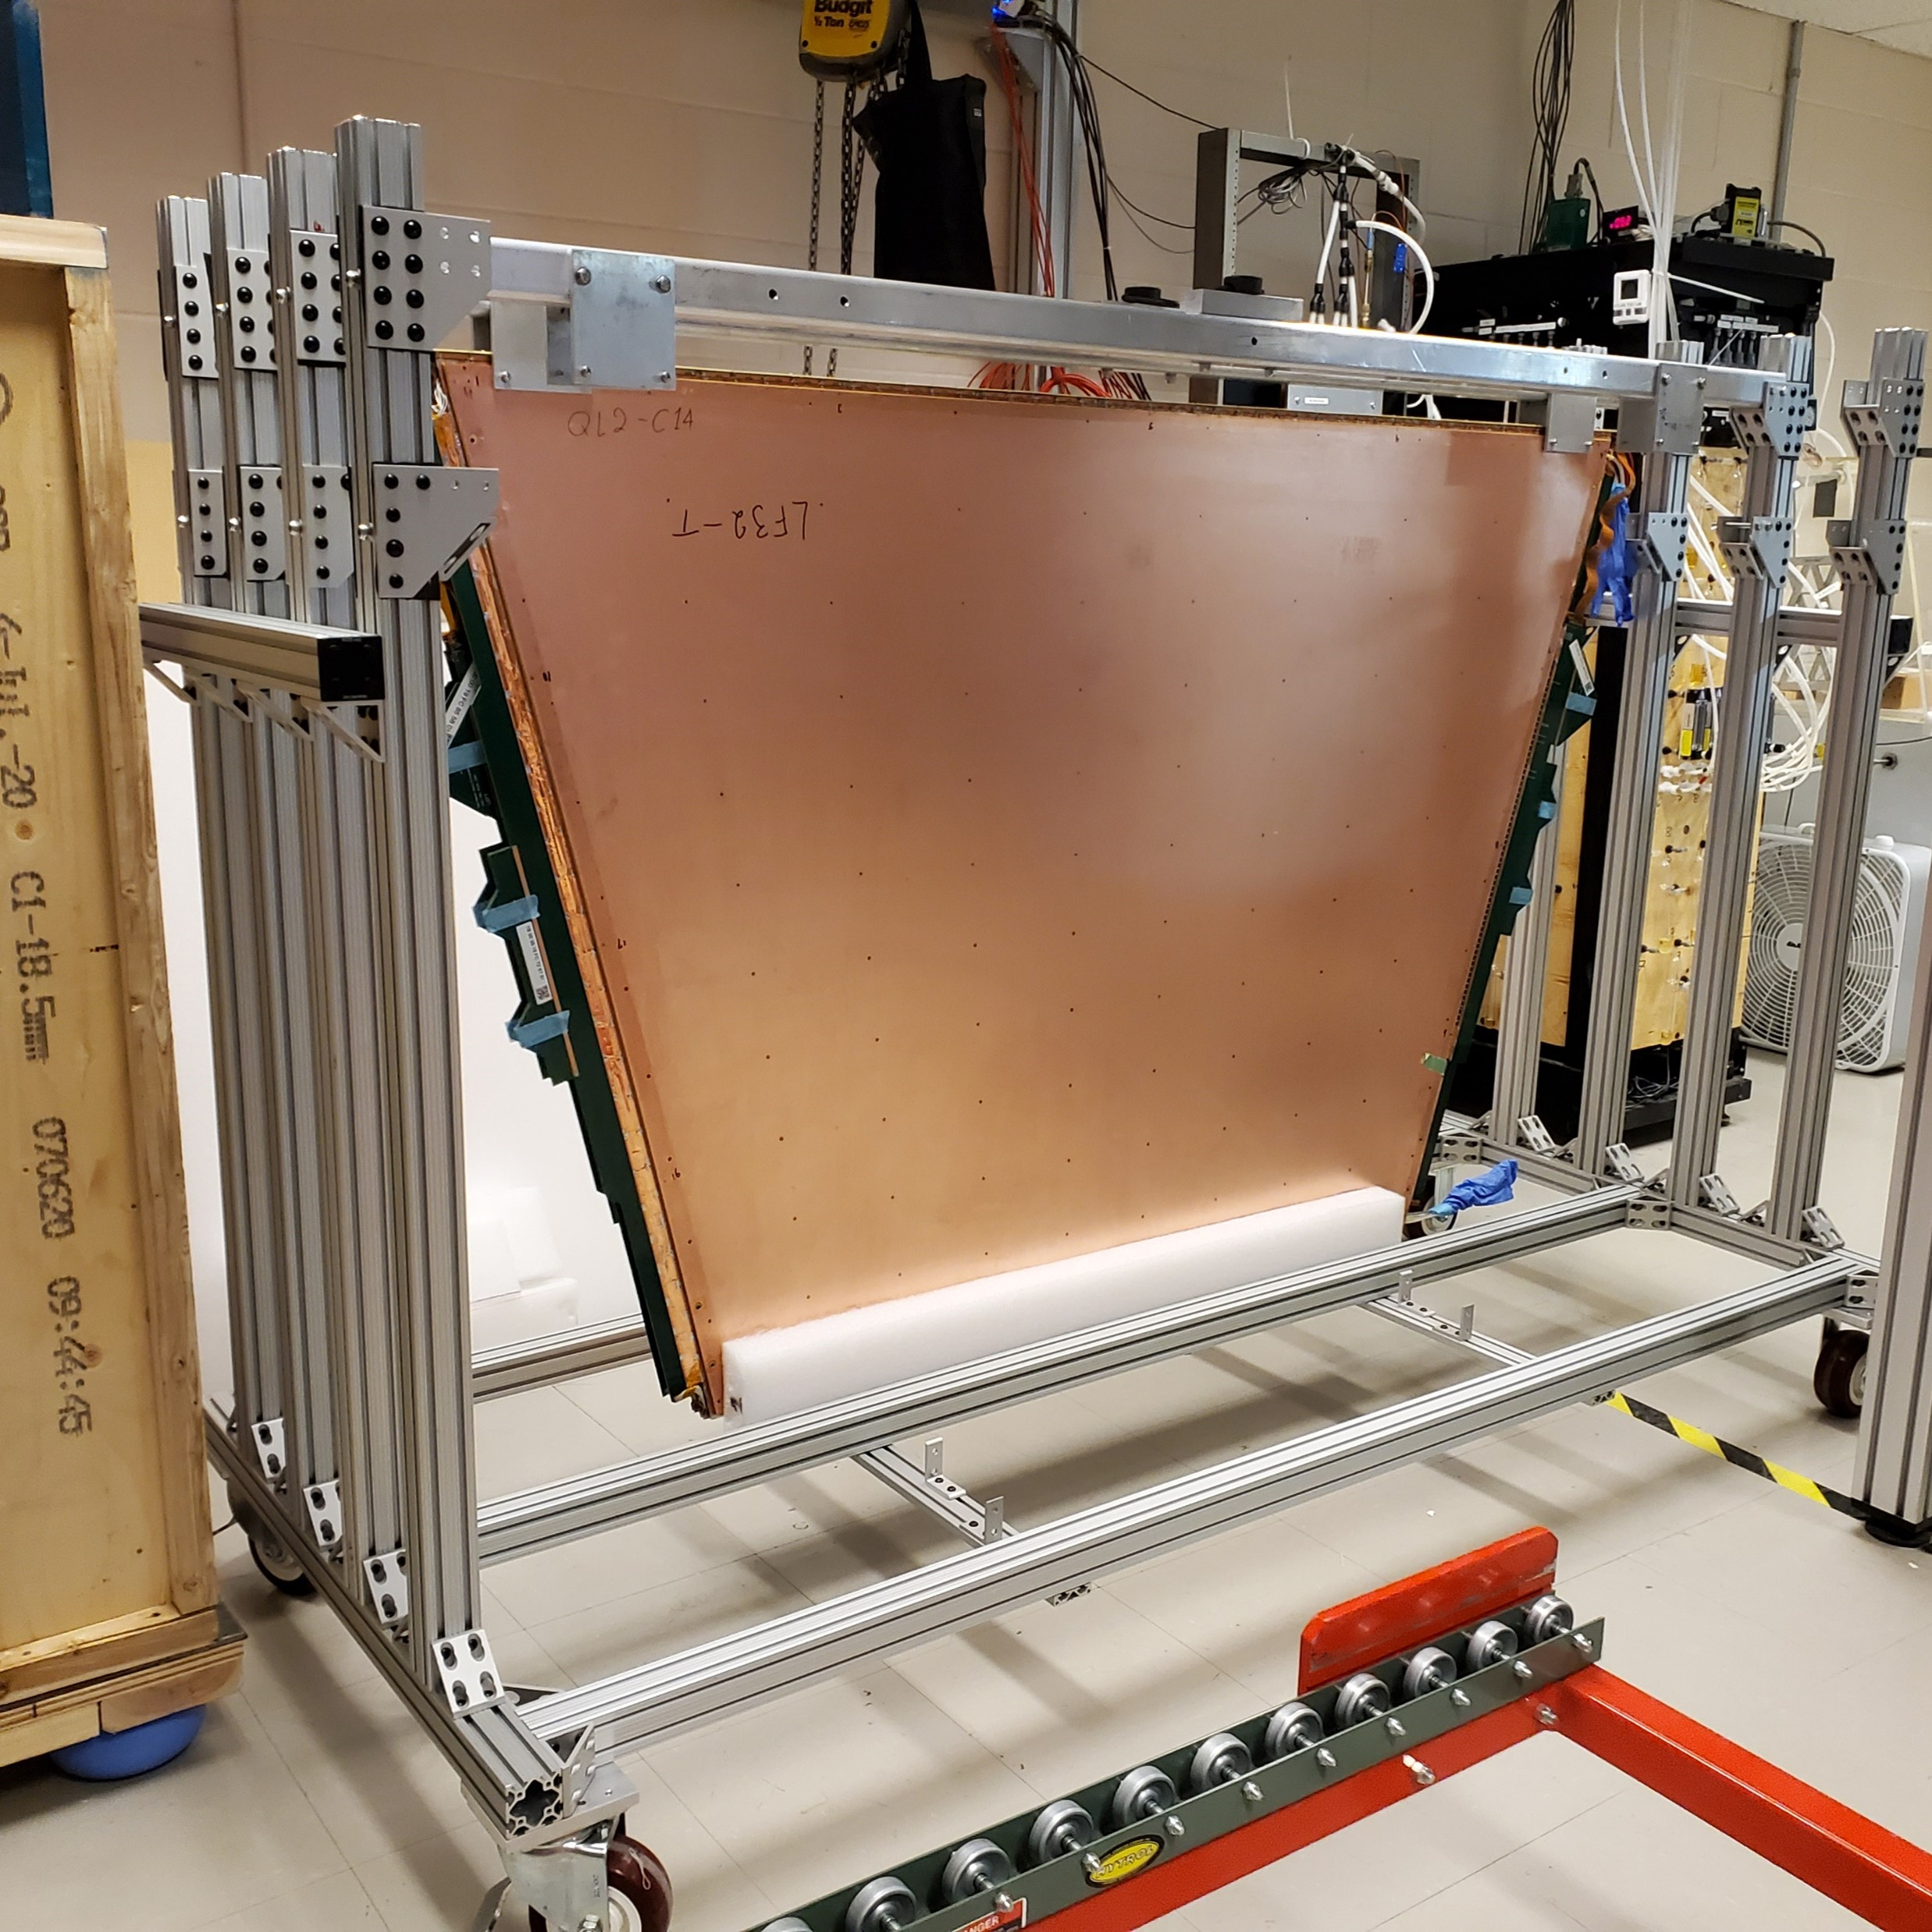
\includegraphics[width=0.35\textwidth]{figures/stgc_quad_cart.jpg}
  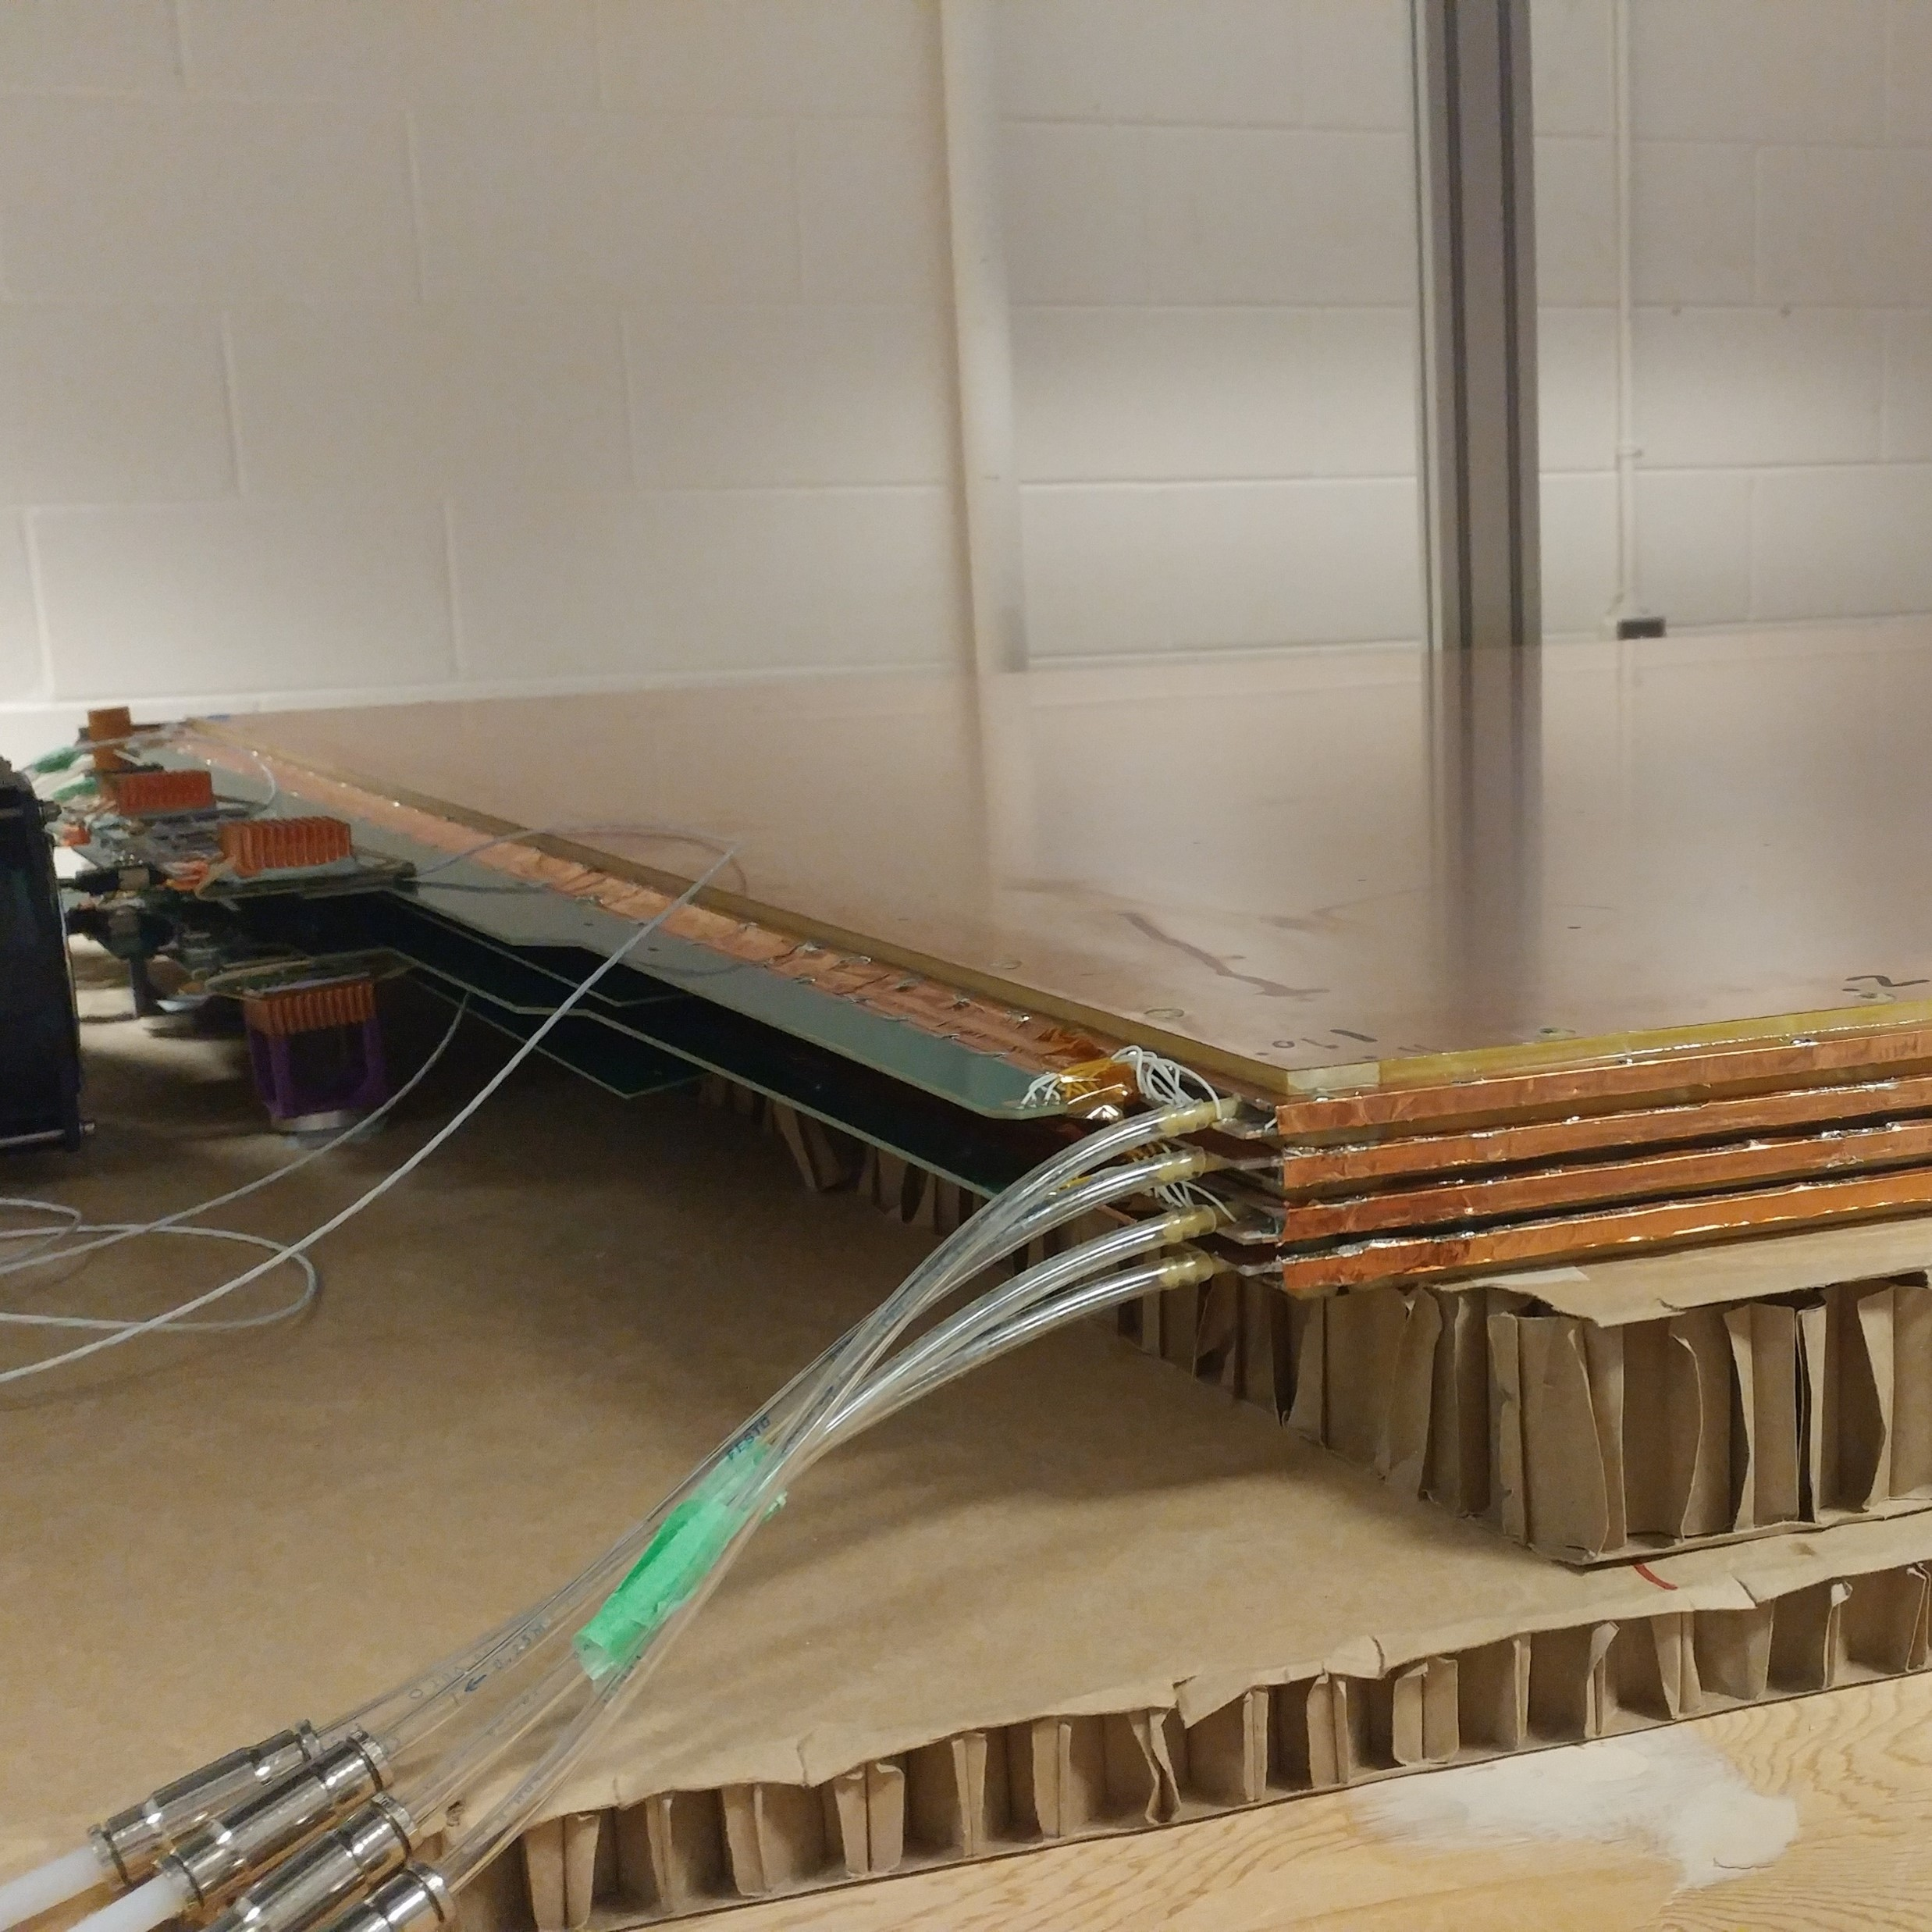
\includegraphics[width=0.35\textwidth]{figures/stgc_quad_inlet_corner.jpg}
  \caption{A sTGC quadruplet module. The left image highlights the trapezoidal shape of a quadruplet module. The right image shows the corner at the short edge, where the four sTGC layers and each layer's gas inlet are visible. The gas outlets and high voltage cables are located along the long edge near the corner in the back left of the photo. The green printed circuit boards along the sides are the adaptor boards where the front end electronics are attached.}
  \label{fig:stgc_quad}
\end{subfigure}

\smallskip

\begin{subfigure}{\textwidth}
  \centering
  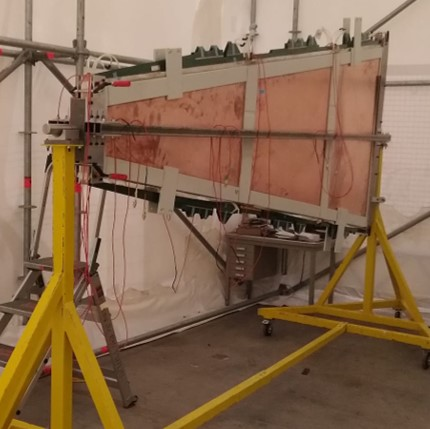
\includegraphics[width=0.35\textwidth]{figures/stgc_wedge.jpg}
  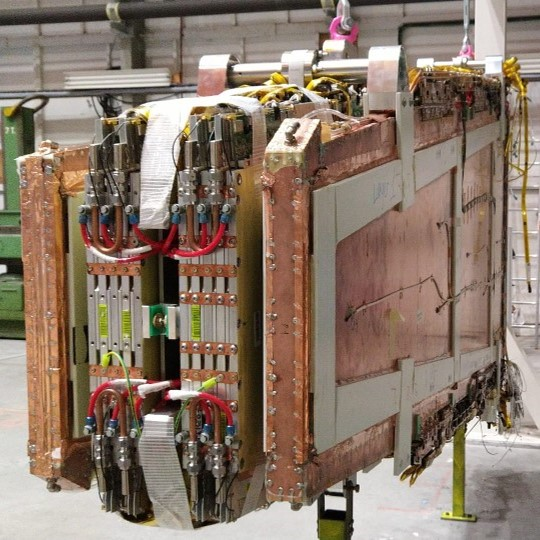
\includegraphics[width=0.35\textwidth]{figures/sector.jpg}
  \caption{Left: A sTGC wedge. The white frame outlines the individual quadruplet modules that have been glued together into a wedge. Right: A completed sector, with two sTGC wedges on the outside and two micromegas wedges on the inside.}
  \label{fig:wedge_and_sector}
\end{subfigure}

\smallskip

\begin{subfigure}{\textwidth}
  \centering
  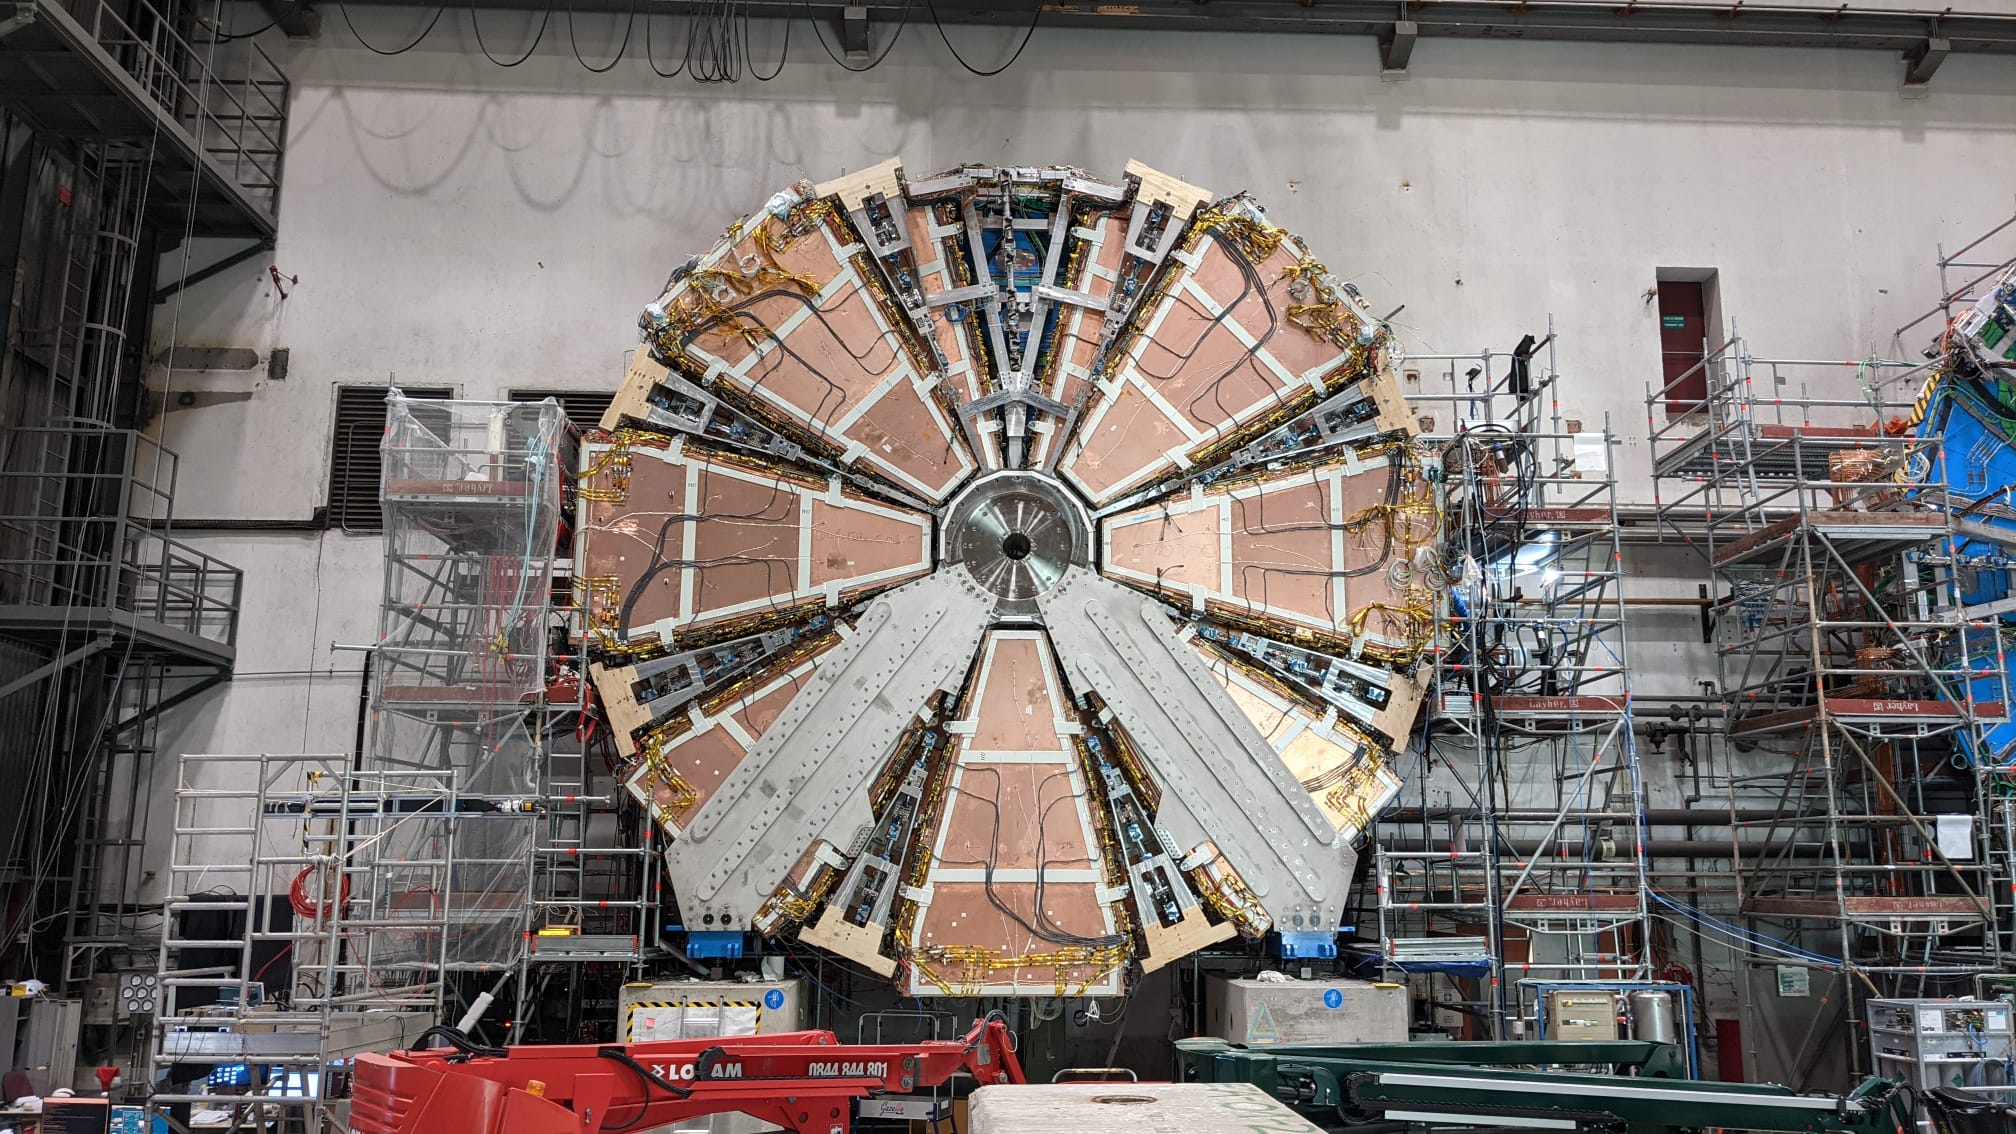
\includegraphics[width=0.7\textwidth]{figures/nsw_2021-05-27_landscape.jpeg}
  \caption{A picture of one of the two NSWs. All sectors except one large sector at the top are installed, revealing two of the smaller sectors that are normally hidden under the large sectors and support bars. The NSWs are \SI{9.3}{m} in diameter. }
  \label{fig:nsw}
  \end{subfigure}
\caption{Images showing different stages of NSW construction.}
\label{fig:nsw_breakdown}
\end{figure}
\newpage
\restoregeometry

% --------------------------------------------------
\section{Design of the NSWs}
% --------------------------------------------------

The NSWs are made with two detector technologies: micromegas and small-strip thin gap chambers. Eight layers of each cover the entire area of the wheel. Micromegas are designed to be the primary precision tracking detectors and sTGCs the primary triggering detectors, but both technologies offer full redundancy by being capable of providing both precision measurements and trigger information. Both types of detectors were designed to achieve spatial resolution better than $\sim$\SI{100}{\micro\meter} per layer. Four chambers are glued together to create quadruplet modules of each detector type. Quadruplets of different sizes, most shaped as trapezoids, are assembled into wedges. Two sTGC wedges and two micromegas wedges are layered to create sectors (with the sTGC wedges on the outside)~\cite{nsw_tdr}. Different stages of the construction process are shown in Figure~\ref{fig:nsw_breakdown}. At the time of writing, the assembly of the NSWs has just been completed. The first NSW has been lowered into the ATLAS cavern and is being commissioned and the second will be lowered shortly. 

% \textcolor{red}{\textit{for if you use computer generated NSW diagram}} Sectors covered the wheel, as shown in figure~\ref{fig:nsw_diagram}. Practically, two different wedge sizes, small and large, were required to completely cover the wheel.
% \begin{figure}
%    \centering
%    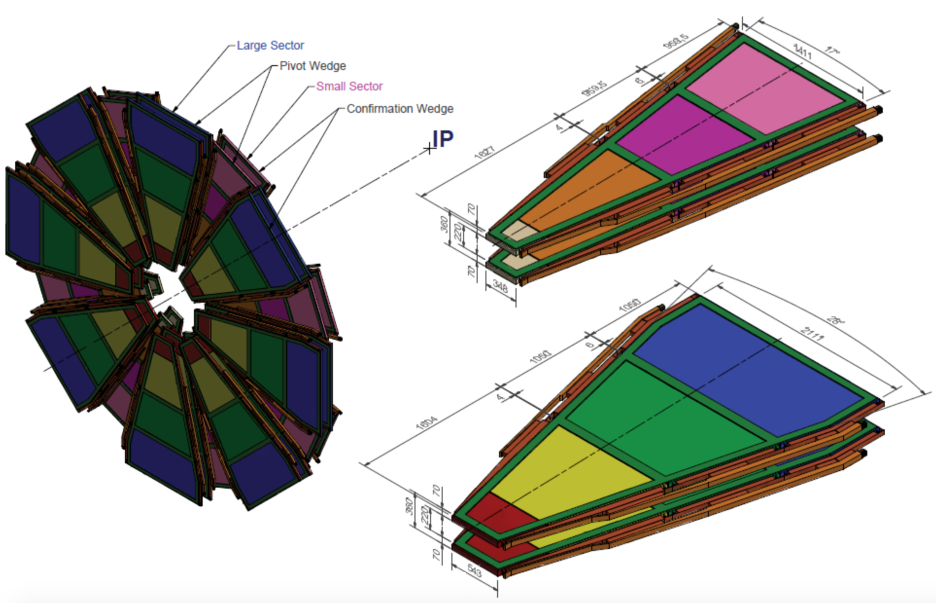
\includegraphics[width = 0.9\textwidth]{figures/nsw_diagram.png}
%    \caption{Drawing of the new small wheel, and diagrams of the individual small and large wedges. Each colour represents a different sTGC module size.}
%    \label{fig:nsw_diagram}
% \end{figure}
% ORIGINAL FULL PAGE NSW SPREAD POSITION

% --------------------------------------------------
% \section{Micromegas}
% --------------------------------------------------

% Micromegas have three components: a drift plane, a gas gap, a mesh, and readout strips, as shown in figure~\ref{fig:micromega}. High voltage is applied to the readout strips. An ionization event in the gas causes electrons to drift towards the mesh. Once they arrived, they are amplified by the strong field and the avalanche is picked up by the readout electrodes. The small distance between the readout electrodes and the mesh, \SI{128}{\micro\meter}, means that positive ions are evacuated in $\sim$\SI{100}{\nano\second}, making micromegas a good choice for high rate environments~\cite{nsw_tdr}. The small pitch of the readout electrodes, \SI{0.425}{mm}, provides spatial resolution much better than \SI{100}{\micro\meter}~\cite{stelzer_new_2016}. MM quadruplets will be used for offline precision tracking~\cite{nsw_tdr}.

% \begin{figure}
%    \centering
%    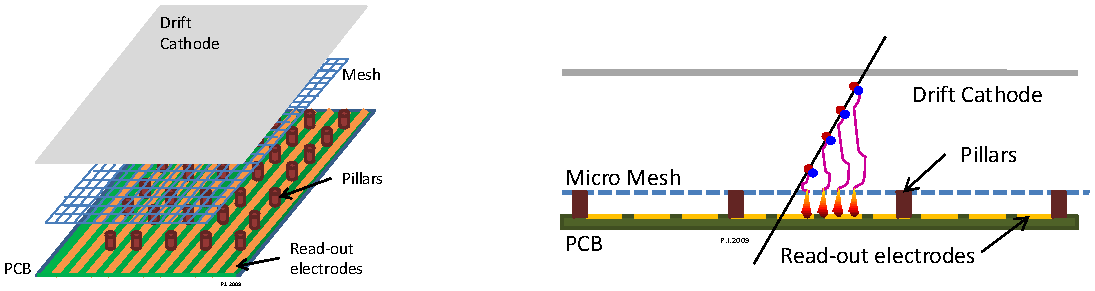
\includegraphics[width = 0.9\textwidth]{figures/micromegas.png}
%    \caption{Sketch the micromega operating principle. Positive high voltage is applied to the readout electrodes, which creates a strong field between the mesh and the readout electrodes, and a weaker field between the mesh and the drift cathode. Amplification takes place between the readout electrodes and the mesh. Figure from~\cite{nsw_tdr}}
%    \label{fig:micromega}
% \end{figure}

% --------------------------------------------------
\section{Small-strip thin gap chambers}
% --------------------------------------------------

\begin{figure}[t]
    \centering
    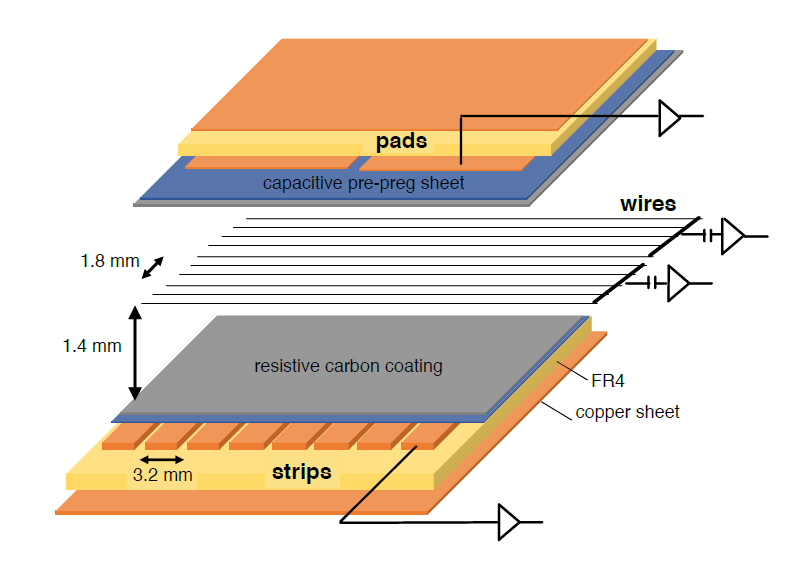
\includegraphics[width = 0.9\textwidth]{figures/stgc_internals.png}
    \caption{Interal structure of an sTGC, zoomed into the area under a pad. High voltage is applied to wires suspended in the gas volume to create an electric field. A passing muon causes an ionization avalache that is picked up by the wire, strip and pad electrodes~\cite{lefebvre_precision_2020}.}
    \label{fig:stgc_internals}
\end{figure}

The sTGCs are gas ionization chambers operated with a gas mixture of CO$_2$:n-pentane with a ratio of 55\%:45\% by volume. Gold-plated tungsten anode wires, \SI{50}{\micro\meter} in diameter and with \SI{1.8}{mm} pitch, are suspended between two cathode planes made of FR-4 printed circuit board, each \SI{1.4}{mm} away (see Figure~\ref{fig:stgc_internals}). One cathode board is segmented into copper pads of varying area (with a typical size of $\sim$\SI{300}{cm^2} each), and the other is segmented into copper strips of \SI{3.2}{mm} pitch running lengthwise perpendicular to the wires. High voltage is applied to the anode wires and the cathode planes are grounded~\cite{nsw_tdr, perez-codina_small-strip_2016}. When a muon passes through a sTGC, it will ionize nearby atoms of the gas. The electrons drift towards the anode wires and in the high electric field region near the wires generate an ionization avalanche~\cite{townsend_electricity_1915}. The motion of the ions and free electrons generates small currents on the nearby wire and capacitatively-coupled strip and pad electrodes~\cite{nsw_tdr}. The gas mixture was chosen to absorb excess photons produced in the avalanche that delocalize the avalanche signal~\cite{majewski_thin_1983} and saturate many strip electrodes, preventing the formation of streamers~\cite{grupen_particle_2008}.  This allows the chambers to be run at a higher high-voltage providing a faster response and higher signal~\cite{majewski_thin_1983}. A carbon coating and pre-impregnated sheet are layered over the printed circuit board of the cathode board, as shown in Figure~\ref{fig:stgc_internals}. The resitivity of the carbon coating and capacitance of the pre-impregnated sheet tune the spread of the charge distribution~\cite{gatti_optimum_1979} and the speed of the response~\cite{battistoni_resistive_1982} to optimize the rate capability. The combined information from the strip readout electrodes and wires provide the location where the muon passed through the chamber. The small pitch of the strip readout electrodes is what allows the quadruplets to deliver good track angular resolution to improve the fake trigger rate and meet the precision tracking requirements~\cite{nsw_tdr}.

% comment on "quick enough to be provided as input to the L1 trigger. Pg. 131 of NSW TDR states req' is under 1025 ns for phase-1, phase-2 will allow longer latency. Latency predictions are shown on pg. 146, but are mostly estimates. Not sure where these latencies are actually measured, nor what the phase-2 requirement is.
A 3-out-of-4 coincidence in pad electrodes from each layer of a quadruplet defines a region of interest where the strip and wire electrodes should be read out. The pad triggering scheme greatly reduces the number of electrodes that require readout so that a track segment of the required angular resolution can be provided quickly enough to the hardware trigger~\cite{nsw_tdr}.

Signal is read out from groups of 20 successive wires, so the position resolution in the direction perpendicular to the wires is \SI{10}{mm} per plane. The wires give the azimuthal coordinate in ATLAS so the position resolution in this direction is sufficient. Good resolution on the $\eta$ coordinate, perpendicular to the strips, is important~\cite{nsw_tdr}. In a test beam environment, the strip spatial resolution of a single sTGC was measured to be 45 microns for muons perpendicularly incident on the surface of the sTGC.  Although the spatial resolution worsens as function of muon angle measured from normal incidence~\cite{lefebvre_thesis}, when four sTGCs are glued together into a quadruplet the design angular resolution of \SI{1}{mrad} in the strip coordinate is achievable~\cite{nsw_tdr, perez-codina_small-strip_2016}. 

To achieve the required track angular resolution once installed in ATLAS, the absolute position of each sTGC strip within the ATLAS coordinate system must be accurately known. The degree of accuracy required is on the order of the position resolution of the chambers, $\sim$\SI{100}{\micro\meter}. The NSW alignment system, detailed in Section~\ref{sec:nsw_alignment}, will monitor the position of alignment platforms installed on the surface of the wedges. The alignment platforms are installed with respect to an external reference on the sTGCs: two brass inserts on each strip layer on one of the angled sides of each quadruplet (shown in Figure~\ref{fig:brasses}). So the challenge of monitoring the position of the strips in ATLAS was separated into two steps: first, infer the position of the strips with respect to the brass inserts using the sTGC design geometry; second, use the alignment system to monitor the position of the alignment platforms. The next section provides some pertinent details on the sTGC construction process, with steps that affect the position of the strips with respect to the brass inserts highlighted.
% The position of the strips can be separated into two stages. First, the NSW alignment system monitors the position of alignment platforms installed on the surface of the wedges, as detailed in section~\ref{nsw_alignment}. Second, the internal geometry of the chambers must be referenced with respect to the wedges. Parts of the sTGC construction process that affect the position of the strips are explained in section~\ref{sec:stgc_construction}. The chapter closes 

\begin{figure}
\centering
\begin{subfigure}{.5\textwidth}
  \centering
  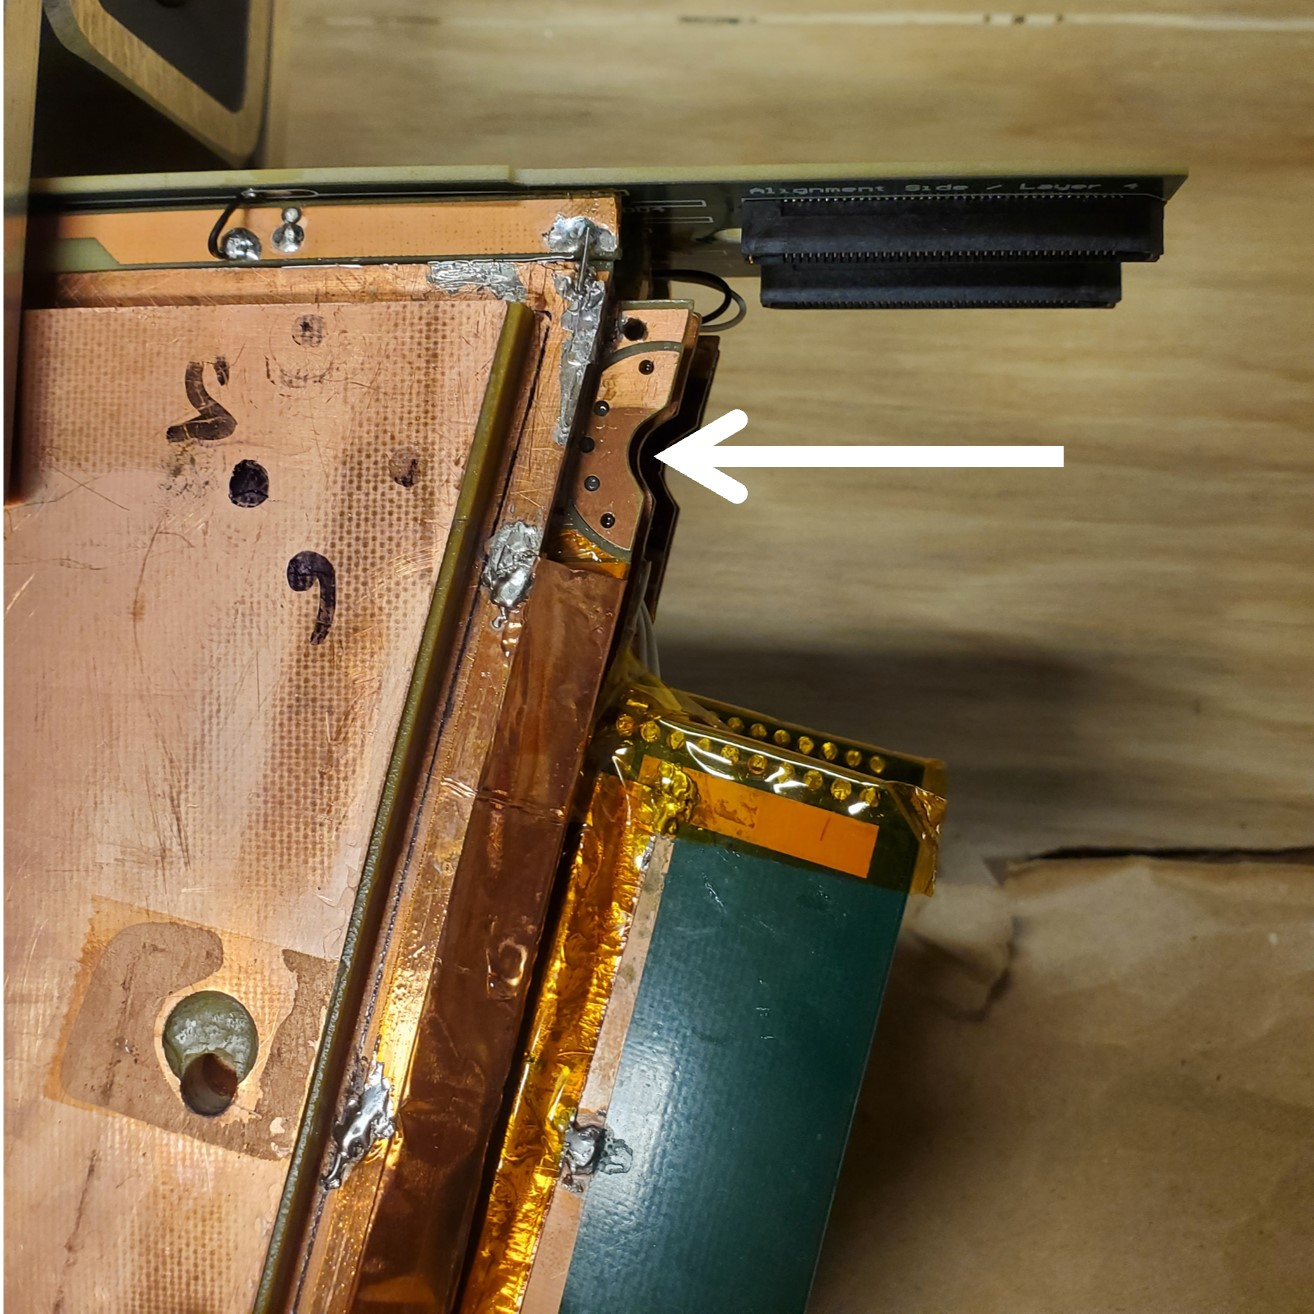
\includegraphics[width=\linewidth]{figures/brass_top.jpg}
  \caption{Brass insert near long edge.}
  \label{fig:brass_top}
\end{subfigure}%
\begin{subfigure}{.5\textwidth}
  \centering
  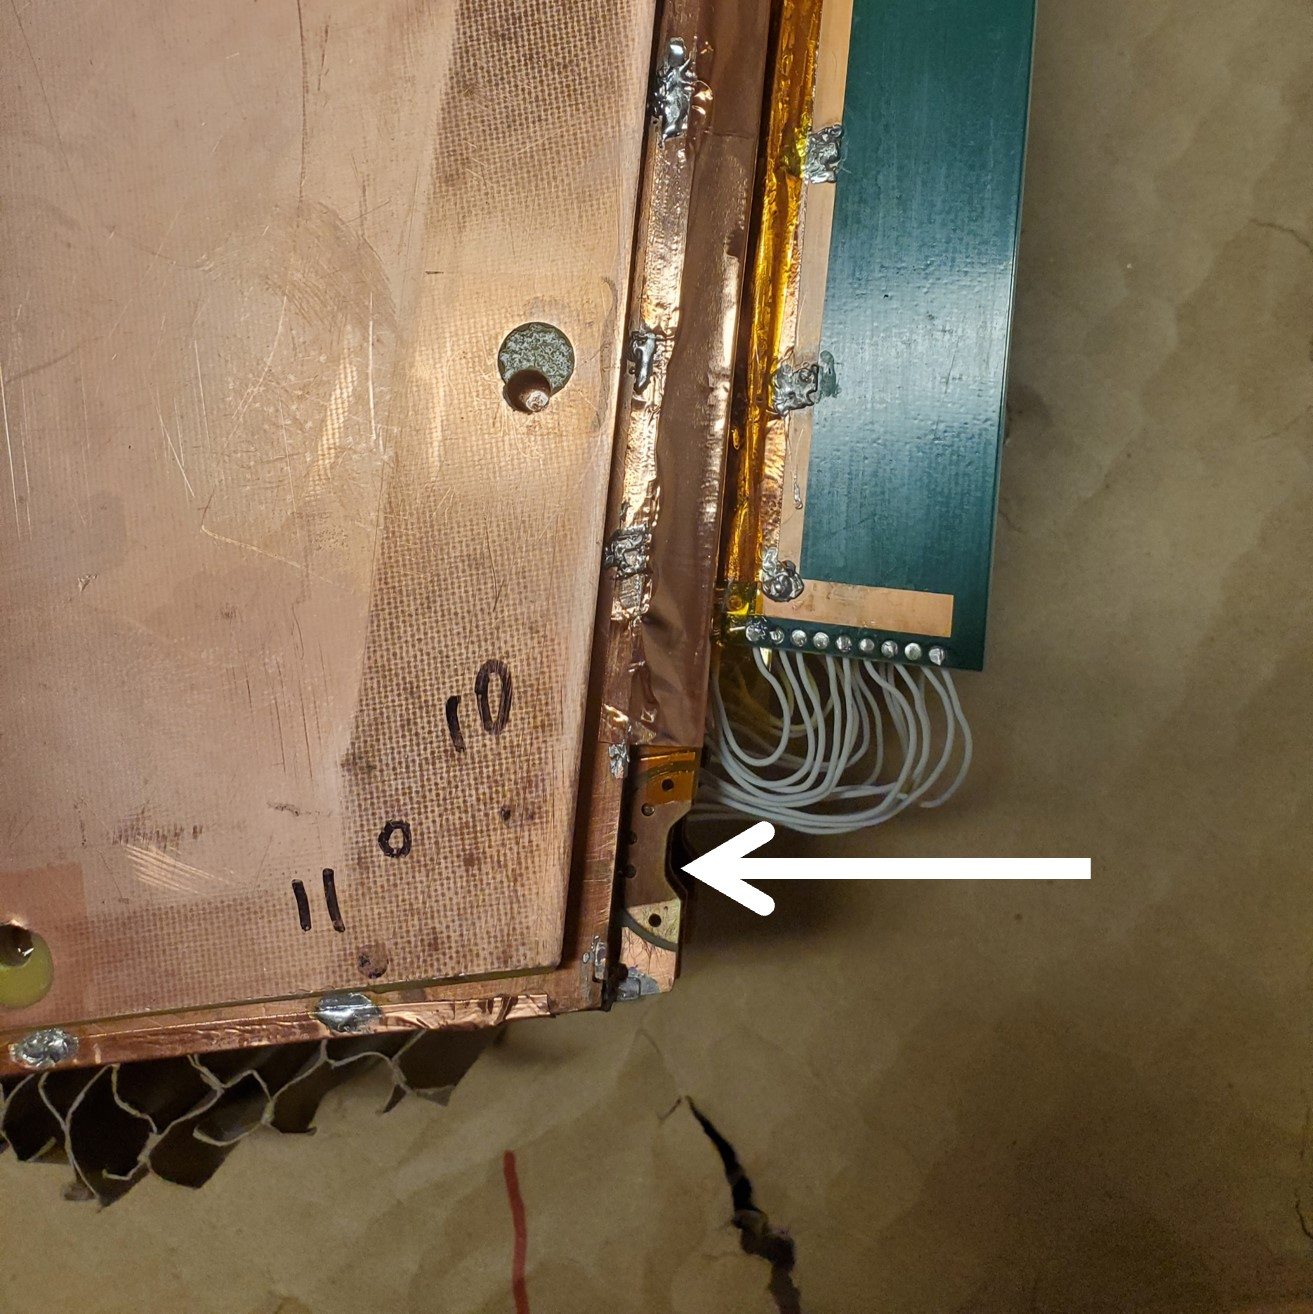
\includegraphics[width=\linewidth]{figures/brass_bottom.jpg}
  \caption{Brass insert near short edge.}
  \label{fig:brass_bottom}
\end{subfigure}
\caption{The brass inserts sticking out from the gas volumes of an sTGC quadruplet. These inserts were pressed against alignment pins when the individual sTGCs were being glued together.}
\label{fig:brasses}
\end{figure}

% However, the accuracy of the hit positions on each layer depends on how well the position of the strips are known in the ATLAS coordinate system. 

% Each strip cathode board has two brass inserts, one near the long edge and one near the short edge, pictured in Figure~\ref{fig:brasses}. The inserts were used to align the strip layers of a quadruplet during construction. They were supposed to control the position of the strips to within \SI{40}{\micro\meter} within nominal. The idea was that the NSW alignment system would monitor the position of points on the surface of an sTGC wedge (discussed in section~\ref{sec:nsw_alignment}) and that the combined external and internal alignment uncertainty on the strip positions would be acceptably small for the precision tracking goals~\cite{nsw_tdr}. Uncontrolled offsets of strip positions on an sTGC layer will bias the reconstructed hit position and hence the track, reducing accuracy of the momentum measurement. To understand the source of offsets in strip positions and misalignments between strip layers, pertinent details of the sTGC construction process are presented in the next section.

% In addition, the sTGC quadruplets should be able to provide precision tracking within \SI{100}{\micro\meter} per plane in the event of a MM module failure.

% --------------------------------------------------
\section{sTGC Quadruplet Construction}
% --------------------------------------------------
\label{sec:stgc_construction}

Five countries were responsible for producing sTGC quadruplets of varying geometries for the NSW: Canada, Chile, China, Israel and Russia. Canada was responsible for the construction of one quarter of the required sTGCs, of three different quadruplet geometries. The steps of the construction process in each country were similar~\cite{nsw_tdr}. The process followed in Canada is detailed here.

A research group at TRIUMF in Vancouver, British Columbia was responsible for preparing the cathode boards. The boards were made and the electrodes etched on at a commercial laboratory, Triangle Labs, in Carson City, Nevada. Once completed they were sent to TRIUMF to be sprayed with graphite and to have support structures glued on~\cite{carlson_results_2019}. The boards are commercial multilayer printed circuit boards, but the strip boards required precision machining to etch the strip pattern~\cite{nsw_tdr}. Triangle Labs also machined the two brass inserts into each strip board. A coordinate measuring machine (CMM) was used to accurately measure the position of a set of reference strips on each board. Four quality parameters describing non-conformities in the strip pattern of each board with respect to the brass inserts were derived from the data and the results are available on a QA/QC database. The parameters~-- offset, angle, scale and nonparallelism~-- and the CMM data collection is described in full in~\cite{carlson_results_2019}.  Due to time constraints, tolerances on the non-conformities in the etched strip pattern with respect to the brass inserts were loosened, with the condition that the strip positions in ATLAS would have to be corrected for~\cite{carlson_results_2019}. 

The prepared boards were sent to Carleton University in Ottawa, Ontario for construction into sTGCs and quadruplets. First, the wires were wound around the pad cathode boards using a rotating table and the wires were soldered into place. A wound pad cathode board was held by vacuum on a granite table, flat to within \SI{20}{\micro\meter}, and a strip cathode board glued on top to create an sTGC. Holding one sTGC flat with the vacuum, another was glued on top to create a doublet, then two doublets were glued together to create a quadruplet. When gluing sTGCs together, the brass inserts were pushed against alignment pins with the goal of keeping the strip layers aligned within tolerance. However, non-conformities in the shape of the brass inserts, non-conformities in the position of the alignment pins and shifts between sTGCs while the glue cured resulted in misalignments between the brass inserts and strip layers. Precise alignment of the pad boards or wires with respect to the strip boards did not have to be so tightly controlled because pads and wires do not measure the precision coordinate. 

The Carleton team finished the quadruplets by installing adaptor boards on the angled sides of each layer that allow front end electronics to be attached. Completed quadruplets were sent to McGill University where their performance was characterized with cosmic rays. Details pertaining to cosmic ray testing of sTGC quadruplets at McGill University are described in Chapter~\ref{chap:cosmics}. Tested quadruplets were sent to CERN where they were assembled into wedges and alignment platforms installed. The alignment platforms were installed using a jig positioned with respect to the brass inserts. Completed wedges were assembled into sectors then installed on the NSWs.

% So, during cathode board construction the etched strip pattern could be shifted off of nominal with respect to the brass inserts. While gluing sTGCs together, non-conformities in the shapes of the brasses and the position of the alignment pins resulted in misalignments between the brass inserts that mean they are not a uniform reference for every layer of the quadruplet. 

The quadruplet construction process had two steps where strip positions could be shifted off nominal. At board-level, there could be non-conformities in the etched strip pattern with respect to the brass inserts, described by the four quality parameters~\cite{carlson_results_2019}. At the quadruplet level, misalignments between the brass inserts and strips on different layers were possibly introduced during the gluing. The result was that the brass inserts were not a reliable reference point and that the strips can be offset from their design position by up to hundreds of micrometers. Offsets in strip positions from nominal in Canadian quadruplets were shown to be random~\cite{carlson_results_2019}, so no one correction would suffice. The offsets must be measured and corrected for in the ATLAS offline software that does the precision tracking. Understanding the work ongoing to make measurements of strip position offsets and correct for them requires understanding the strategy of the NSW alignment system.

% Two sources of misalignment resulted at board level: non-conformities in the placement and shape of the brass inserts and non-conformities in the strip pattern. Carlson addressed the non-conformities in the strip pattern of Canadian cathode boards in his thesis~\cite{carlson_results_2019}. A coordinate measuring machine (CMM) or FaroArm was used to digitize the etched strip pattern of each board. Four quality parameters describing non-conformities in the strip pattern were derived from the data and the results are available on a QA/QC database. The parameters were offset, angle (rotation), scale and non-parallelism, defined in ful in Carlson' thesis. Often, alignment models only consider an offset and rotation. 

% Once the cathode boards were prepared, they were sent to TRIUMF in Vancouver, British Columbia to be sprayed with the graphite coating. After spraying, the coating was polished until the resistivity was between 90 and \SI{110}{\kilo\ohm}$/\msquare$, then wire support structures and frames were installed~\cite{nsw_tdr}. The completed boards were sent to Carleton university for construction into gas gaps and multiplets.

% First, anode wires were wound onto the the pad cathode boards using a rotating vacuum table. Then, a pad and strip cathode board has to be glued together to create an sTGC, two sTGCs glued together to create a doublet, and two doublets glued together to create a quadruplet. Gluing was done by holding one side of a cathode board in place with vacuum on a granite table, flat to within \SI{20}{\micro\meter}. A honey comb spacer separates each sTGC layer of a quadruplet. When closing a gas gap, micrometer misalignments between the strip and pad cathode boards do not matter since the pads do not measure precision coordinates. When gluing sTGCs into doublets however, alignment between strip layers had to be controlled by pushing the two brass inserts against alignment pins~--- similarly for gluing together doublets. Once a quadruplet was assembled, adapator boards used to route the electrodes' signals to the front end electronics were soldered on to the angled sides of the quadruplet~\cite{nsw_tdr}. 

% If you want to include the x-ray survery of the brass positions and the microscope method
% At every stage in the process quality control checks were in place for gas, high voltage, and alignment. For alignment, \textcolor{red}{the position of the brasses were recorded in 3D using an x-ray gun~\cite{nsw_tdr} \textit{--> Did this actually happen?}}~\cite{nsw_tdr} and alignment between strips visible outside a quadruplet was checked with a microscope~\cite{carlson_results_2019}. 

% Quality control tests of alignment, ability to hold high voltage, gas sealing etc. were undertaken at every stage in the construction process~-- details can be found in~\cite{nsw_tdr}. The final set of quality control checks and characterization was done at McGill University in Montreal, Quebec. Completed quadruplets were tested for gas leaks, noise and characterized with cosmic rays. The details of cosmic ray testing are described in chapter~\ref{chap:cosmics}.

% Once the quadruplets have been tested with cosmics rays, they are sent to CERN to be further tested, assembled into wedges then sectors, then installed on the NSWs. At the time of writing, all sectors have been installed on both wheels. The first NSW has been lowered into the ATLAS cavern and is being commissioned. The second is scheduled for installation in October, 2021.

% --------------------------------------------------
\section{NSW alignment}
% --------------------------------------------------
\label{sec:nsw_alignment}
% The idea of the NSW alignment system is presented in~\cite{nsw_tdr}, but the details have only been presented internally so far. The original goal of the alignment system was to provide the position with respect to one another of any three chambers traversable by a muon track with an accuracy of \SI{40}{\micro\meter} in the precision coordinate~\cite{nsw_tdr}. Likely for sTGCs, this will mean inputing the strip postions, or parameters to calculate the strip positions, into the ATLAS experiment's offline software, \package{Athena}.

The idea of the NSW alignment system is presented in~\cite{nsw_tdr}, but the details have only been presented internally so far. After the wedges are constructed, alignment platforms are installed on every sTGC quadruplet and optical fibres routed to them, as shown in Figure~\ref{fig:alignment_platforms}. Light from the optical fibres will be monitored in real time by cameras (BCAMs) mounted on the alignment bars of the NSWs. The system will thus record the positions of the alignment platforms in the ATLAS coordinate system and any changes over time. % The final link in the sTGC alignment system requires knowing the position of the strips inside a chamber with respect to the alignment platforms.

\begin{figure}[h]
    \centering
    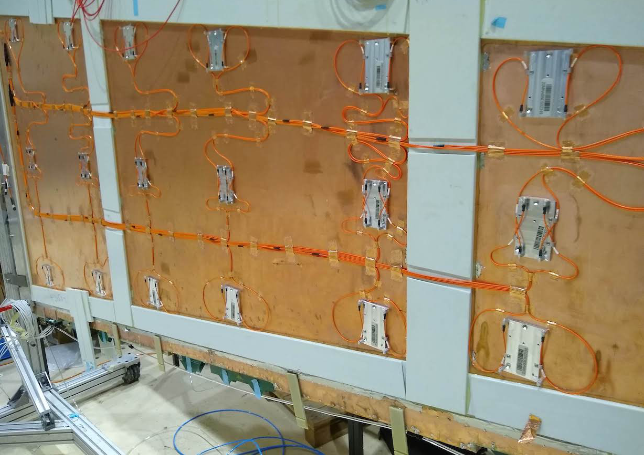
\includegraphics[width = 0.75\textwidth]{figures/alignment_platforms_lefebvre.png}
    \caption{A sTGC wedge with alignment platforms (silver) installed on the quadruplet. Optical fibres (orange) are routed to the alignment platforms. Cameras on the frames of the NSWs will record light from the optical fibres to monitor in real-time the position the alignment platforms in the ATLAS coordinate system.}
    \label{fig:alignment_platforms}
\end{figure}

% If you want to mention the alignment jig in the last paragraph:
% They are positioned with the help of an alignment jig, which is like a frame that can be positioned on top of a wedge with cut outs indicating the correct position for the alignment platforms. The jig is positioned with respect to the brass inserts \textcolor{red}{[Benoit 2020-01-20, 2020-04-16 presentations]}.

% The goal was to control the position of the strips in the chamber to within ~\SI{40}{\micro\meter} for precision tracking goals~\cite{nsw_tdr} --- then knowing the position of the brass inserts with respect to the alignment platforms would allow the strips to be positioned accurately enough. That is the alignment scheme shown in solid arrows in figure~\ref{fig:alignment_elements}. Due to time constraints, tolerances on the non-conformities in the etched strip pattern were loosened, with the condition that the strips positions would have to be corrected for in the software~\cite{carlson_results_2019}. Then, non-conformities in the brass inserts, misalignment of the pins the brass inserts were pushed against, and shifts of the strip layers while the glue was curing resulted in misalignments between the brass inserts~-- and between the strips layers ~-- that prevent using the brasses as an external reference of the position of the strips. The misalignments between Canadian sTGCs were shown to be random~\cite{carlson_results_2019}, so no one correction would suffice.

% The original alignment scheme was to use the brass inserts as a reference between the alignment platforms and the individual strips, as shown in the solid arrows in figure~\ref{fig:alignment_elements}. \textcolor{red}{Due to time constraints, tolerances on the non-conformities in the etched strip pattern with respect to the brass inserts were loosened, with the condition that the strips positions would have to be corrected for. Corrections will happen in ATLAS offline software, \package{Athena}, that will do the precision tracking~\cite{carlson_results_2019}. --> MOVE THIS} Moreover, non-conformities in the shape of the brass inserts and the alignment pins added misalignment between the inserts of different layers~-- and between the strips of different layers~-- that prevent using the brass inserts as a reference. Offsets in strip positions from nominal in Canadian quadruplets were shown to be random~\cite{carlson_results_2019}, so no one correction would suffice.

\begin{figure}
    \centering
    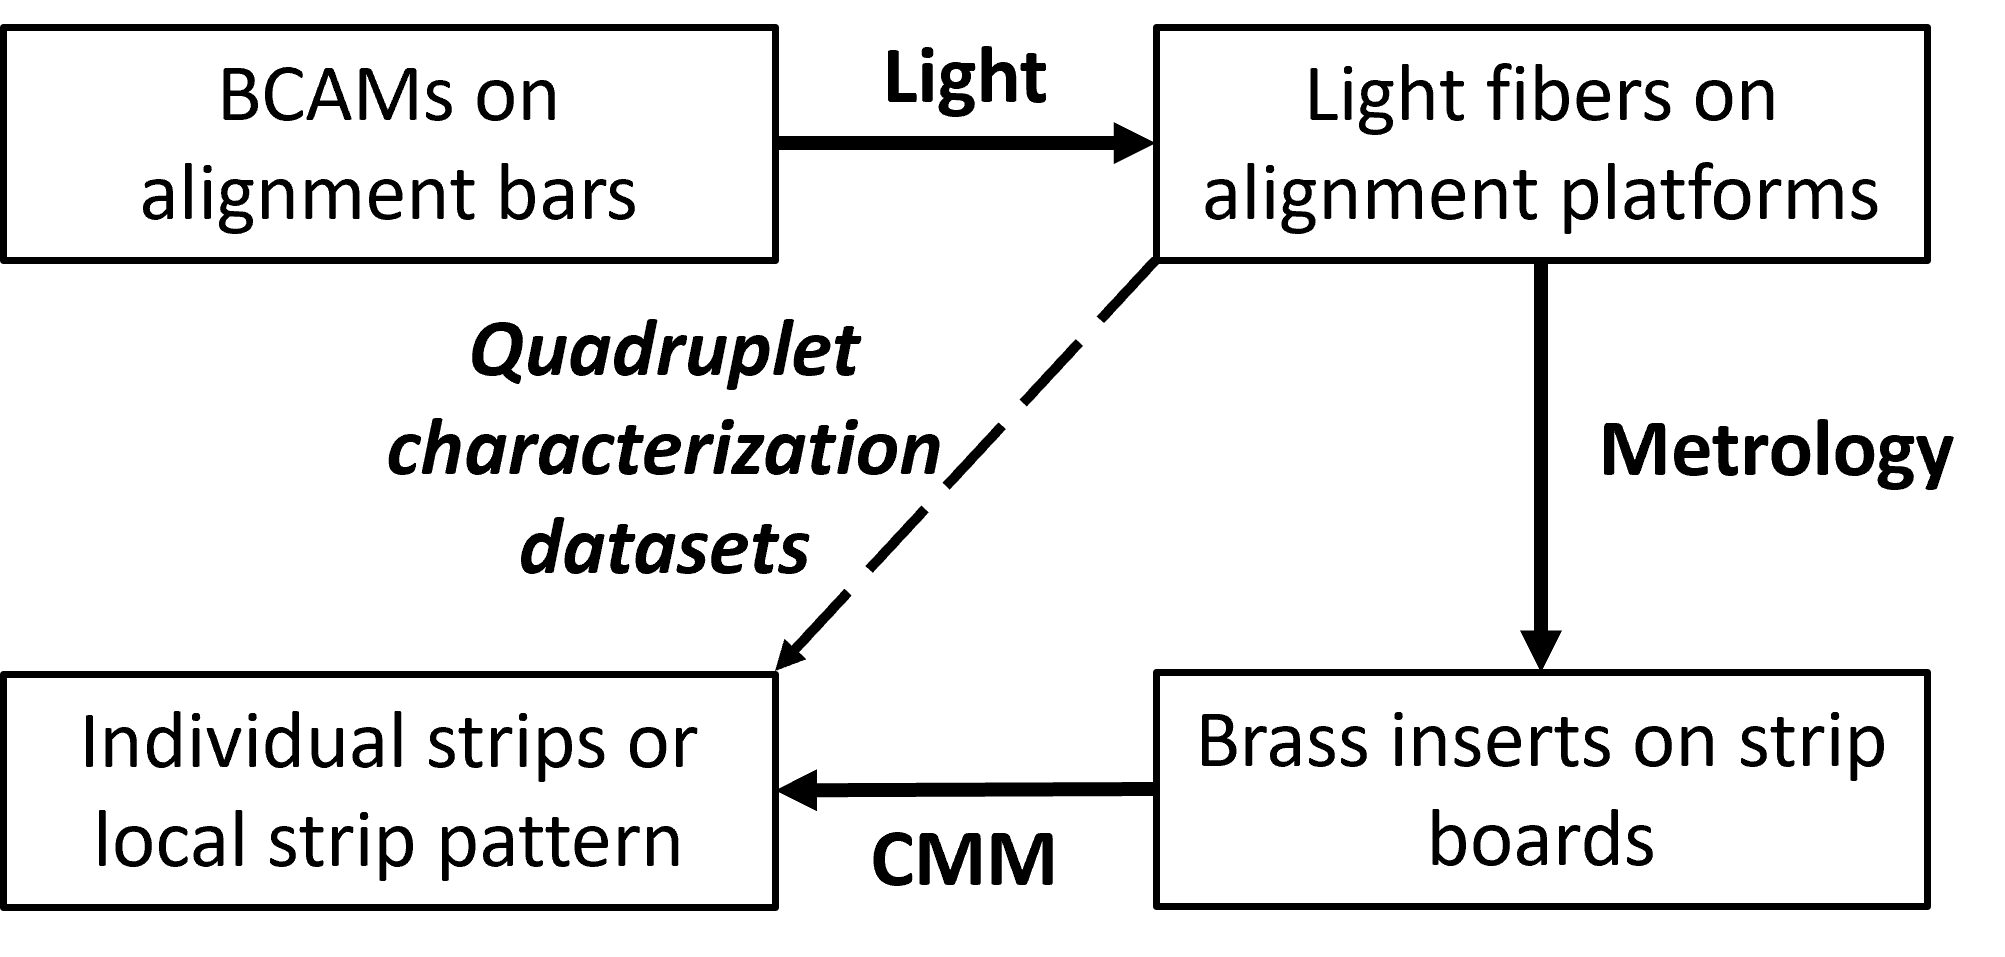
\includegraphics[width = 0.9\textwidth]{figures/alignment_system_element_relations.png}
    \caption{Schematic diagram showing how the different elements of the sTGC alignment system relate to one another. The solid arrows denote the planned alignment scheme. The dashed arrow shows the modification being finalized now. This figure was originally designed by Dr. Benoit Lefebvre.}
    \label{fig:alignment_elements}
\end{figure}

The original alignment scheme was to use the brass inserts as a reference between the alignment platforms and the individual strips, as shown in the solid arrows in Figure~\ref{fig:alignment_elements}~-- this will no longer work. The position of the alignment platforms will be known thanks to the alignment system, so a different method to get the position of the strips with respect to the alignment platforms is currently in its final stage of development. The technique consists of the measurement of the strip pattern offset at a few areas on the surface of a sTGC quadruplet using an xray gun mounted on the alignment platforms. The local strip pattern offset with respect to nominal geometry at the location of each alignment platform is obtained by analyzing the xray gun beam profile. As shown in Figure~\ref{fig:alignment_elements}, this approach essentially bypasses the need to know the position of strips with respect to the brass inserts. The alignment platforms provide the link to the nominal geometry because the nominal group of strips that should be nearest to them can be identified using the nominal geometry parameters that assume the strips are perfectly etched and aligned. Cosmic muon track positions cannot be compared to the nominal geometry because the alignment platforms are not installed when cosmics data is collected, so there is no external reference to provide a link to the nominal geometry.

The x-ray method does not have the sensitivity to measure the offset of each strip from nominal, but what can be measured instead is the offset of the strip pattern in a local area around the position of the gun. \textit{Local offsets} are used to build an alignment model for each strip layer. Formally defined, an alignment model is a set of parameters used to estimate the ``as-built'' position of a strip given its nominal position. The alignment model currently being worked on takes x-ray and CMM data as input to calculate an overall offset and rotation of each strip layer with respect to nominal~\cite{lefebvre_precision_2020}. The alignment parameters could be described as ``global'', meaning over the whole layer instead of local. Without the x-ray dataset, there would be no input to the alignment model that takes into account inter-layer misalignments introduced during quadruplet construction.

Given that the x-ray local offsets can only be measured at positions where the gun can be attached and that they are an important part of the alignment scheme, the new x-ray measurement technique needs to be validated. The goal of this thesis is to validate the x-ray local offsets while exploring how cosmics data complements and adds to the understanding of strip positions and global alignment.

% --------------------------------------------------
% \section{Thesis motivation}
% --------------------------------------------------
%\textcolor{red}{It feels right to remind people of the goal of this work here, even though this is done in the introduction. Options: keep this section, remove this section; move the first two sentences of this section to the end of the NSW alignment section above for a briefer reminder. Thoughts?}

% Given that the x-ray local offsets can only be measured at positions where the gun can be attached and that they are an important part of the alignment scheme, the x-ray method needs to be validated. The goal of this thesis is to validate the x-ray local offsets while exploring how cosmics data complements and adds to the understanding of strip positions and overall alignment. Chapter~\ref{chap:lhc_atlas} presented the physics motivation of the HL-LHC and chapter~\ref{chap:nsw} motivated the NSW upgrade and the importance of alignment. Chapter~\ref{chap:cosmics} explains how cosmic muon data is collected, how it is used to calculate relative local offsets, and what information it gives about alignment. Chapter~\ref{chap:xray} explains how x-ray data is collected, how it is used to calculate local offsets, and how relative local offsets can be calculated for comparison to cosmics. Chapter~\ref{chap:comparison} compares the results of the two methods; and chapter~\ref{chap:outlook} contextualizes the results in terms of the alignment model and alignment system.

% Snippets
%The main dataset was collected using x-rays as the probe. The x-ray data has been combined with the CMM data to create an alignment model that can be used to estimate the position of each strip. The goal of this work was to validate the measurements of strip pattern offsets done with the x-ray dataset with the cosmic muon data. Currently, only modules made in Canada have been analyzed in this way, but the method applies for other countries that were able to collect cosmic muon data on multiple quadruplet layers. 

%Moreover, as-built alignment parameters must be measured and extracted to ensure proper function and provide a way to correct for misalignment. The next section breaks down the sTGC construction process to highlight the stages of alignment.
%All countries successfully finished delivering their modules this year, and the sectors have been installed on the NSWs. 































% ==================================================
% CHAPTER 5: Using cosmic muons to measure relative strip position offsets %
% ==================================================

\chapter{Using cosmic muons to measure relative strip position offsets}
\label{chap:cosmics}
% Edit count: Lia - 0, Brigitte - 0

At McGill University, among other quality and functionality tests, each Canadian-made quadruplet was characterized with cosmic muons. In this chapter, the experimental setup and how the data was analyzed to provide relative strip position offsets is presented. The analysis method was motivated by the how the measurements could be compared to measurements done with the x-ray method (Chapter~\ref{chap:xray}) but also it stands alone as a characterization of the alignment between strips of different layers. The chapter begins with a brief introduction to cosmic rays.

% --------------------------------------------------
\section{Cosmic rays}
% --------------------------------------------------

The earth is being constantly bombarded by particles from the sun, galactic sources and extra galactic sources~-- collectively called cosmic rays~\cite{boezio_chemical_2012, zyla_review_2020}. Cosmic rays consist mostly of protons, but also heavier ions, gamma rays and the term sometimes includes neutrinos. The primary (initial) cosmic ray interacting with the atmosphere causes electromagnetic and hadronic showers of secondary particles. Hadronic showers result from the primary cosmic ray interacting strongly with the target of the atmosphere, resulting in an abundant production of pions. Charged pions predominantly decay to muons (there is a lesser contribution to the muon flux from kaons as well)~\cite{grieder_cosmic_2001}. The secondary muons are relativistic and thanks to time dilation their lifetime is extended as measured in the reference frame of earth, so a flux of approximately 1 muon\SI{}{\per\cm\squared\per\min} reaches the ground~\cite{zyla_review_2020}. Measuring the muon flux and energy spectrum reveals information about primary cosmic rays~\cite{grieder_cosmic_2001} which is interesting to high energy physicists and astrophysicists. The muon flux is also terribly convenient for testing muon detectors.

% --------------------------------------------------
\section{Experimental setup}
% --------------------------------------------------

\begin{figure}[h]
    \centering
    \includegraphics[width = 0.9\textwidth]{figures/figure_test_bench.png}
    \caption{Cosmic muon hodoscope at McGill University with a sTGC quadruplet module in the test bench.}
    \label{fig:hodoscope}
\end{figure}

Cosmic muon characterization of sTGC quadruplet modules was done with a hodoscope, a complete description of which can be found in~\cite{lefebvre_thesis}. The quadruplet was placed in the center of the test bench. Above and below it was a layer of scintillator-PMT arrays, as shown in Figure~\ref{fig:hodoscope}. When a cosmic muon passed within the acceptance of the hodoscope, at least one scintillator from the top array and at least one from the bottom array fired in coincidence. A trigger signal was formed using NIM modules from the coincidence of signals from the top and bottom arrays of scintillators. The trigger signal was passed \iffalse through a KC705\footnote{Xilinx, Xilinx Kintex-7 FPGA KC705 Evaluation Kit, EK-K7-KC705-G, 2018} which sent it \fi to the front-end electronics attached to the adaptor boards of each layer of the quadruplet.

Operating the chambers also required gas and high voltage. A gas mixture of pentane-CO$_{2}$ in the appropriate proportions was prepared and delivered to each sTGC with a gas system designed and made at McGill University~\cite{keyes_development_2017}. Since pentane is flammable, the gas system was designed with safety top of mind. The gas system was controlled by a slow control program, also custom made~\cite{keyes_development_2017}. To prepare the quadruplets for operation, CO$_{2}$ was flushed through them overnight to remove potential impurities within each chamber's gas volume. Then, the equivalent of approximately five sTGC gas volumes of the pentane-CO$_{2}$ mixture was flushed through to ensure a uniform gas mixture inside the sTGCs; the procedure takes approximately four hours. High voltage was provided by commercial CAEN high voltage boards~\cite{keyes_development_2017}. 

% About 2.9 kV vs 3.1 kV
%Although the chambers will be operated at 2.8~kV in ATLAS, the earlier version of the FEBs used at McGill had a worse signal-to-noise ratio for pads, which was compensated for operating the chambers at \SI{3.1}{kV}, which increased the chambers' gain. Operating at \SI{2.9}{kV} was sufficient for strip and wire signals and closer to the nominal voltage. Collecting 1 million triggers at each voltage provided enough statistics to calculate characterization metrics, which meant collecting data for just over two hours per quadruplet per voltage.

% --------------------------------------------------
\section{Data acquisition}
% --------------------------------------------------
% It would be great to have a scope trace here, preferably of a strip. Oops.
Each sTGC electrode was connected to a channel on a prototype ASIC\footnote{A custom Application Specific Integrated Circuit (ASIC) named VMM3~\cite{iakovidis_vmm3_2017}, designed for the readout of signals from the micromegas and sTGCs of the NSWs.} on the front-end electronics, attached to the adaptor boards on each layer of a quadruplet. Each ASIC features 64 charge amplifiers with selectable gain and input signal polarities, which output the digitized amplitude of the signal at peak for channels above a pre-defined threshold. Thresholds were estimated~\cite{chen_calibration_2019} by optimizing the efficiency of detecting muons while minimizing noise, and further manually tuned in the configuration/readout software before the start of data acquisition for each quadruplet. The signal from the capacitively-coupled strip electrodes has positive polarity and is read out with a gain of one. For each trigger, the signal peak amplitude of all channels above threshold was recorded  as an event and stored in a binary file. The readout of strips made use of a special feature of the custom ASIC, the so-called ``neighbour triggering'' function where signals on channels adjacent to those above threshold are also read out.

The quadruplets were held at \SI{3.1}{kV} for approximately two hours to collect data from approximately 1~million muon triggers.

% --------------------------------------------------
\section{Data preparation}
% --------------------------------------------------
\subsection{Data quality cuts on electrode hits}
\label{subsec:hit_cuts}
Corrupted data, if any, is removed while the raw data is being recorded in a binary file. After data taking is completed, the raw data is decoded and the electronics channels are mapped to physical readout electrodes of the quadruplet. The result of this data preparation step is stored in a \package{ROOT}~\cite{ROOT_paper} tree data format. 

A hit is defined as a signal recorded from a channel that was above threshold or (in the case of strips) neighbour triggered. In addition to hits from muons, the quadruplets record noise from the electronics and $\delta$-rays (electrons liberated with sufficient energy to escape a significant distance away from the primary radiation and produce further ionization). Therefore, selection cuts are applied to reduce the number of hits that do not originate from muons. Readout strips located at the very edge of the cathode board tend to have higher electronic noise.  As a result, all strip hits on a layer where a hit is present on the strips at either edge of the quadruplet are removed from the analysis. A default pedestal value is subtracted from the recorded signal peak amplitude of each electrode for a more realistic estimate of the signal amplitude. Also, events that only have hits on pad electrodes (no strips or wires) were removed from the analysis since these hits are likely from electronic noise, which is higher on the pad readout channels due to their large area.

% --------------------------------------------------
\subsection{Clustering and tracking}
% --------------------------------------------------
\label{subsec:clustering}
For events passing the quality selection cuts defined in Section~\ref{subsec:hit_cuts}, the $x$- and $y$-coordinates of the ionization avalanche on each layer are extracted from the signal on the wires and strips respectively for each event, as shown schematically in Figure~\ref{fig:mwpc_coords}. In this work, $x$ is defined as the coordinate perpendicular to the wires and $y$ is defined as the coordinate perpendicular to the strips. The $z$-coordinate is perpendicular to the sTGC surface.

The $x$-coordinate of the muon position is taken as the center of the wire group with the maximum peak signal amplitude, since the wire groups' pitch (\SI{36}{\milli\meter}) is larger than the typical extent of the ionization charge generated inside a sTGC. Assuming that the true $x$-position of the hit is sampled from a uniform distribution over the width of the wire group, the uncertainty in the x-position is approximately $\frac{36}{\sqrt{12}}$~mm~=~10~mm~\cite{Sauli:117989}.

\newpage
\thispagestyle{empty}
\newgeometry{top=0.5in,bottom=0.5in}
\begin{figure}
    \centering
    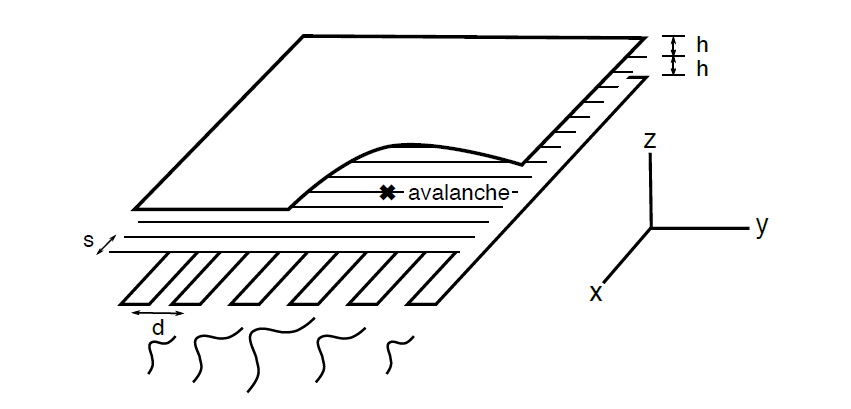
\includegraphics[width = 0.8\textwidth]{figures/mwpc_lefebvre_thesis_gatti.png}
    \caption{Schematic diagram representing the three types of electrodes in a sTGC detector. The position of the ionization avalanche is extracted from the wires and strips that picked up the avalanche signal. The signals on individual strips are sketched. Clustering is the process by which a Gaussian function (represented by the grey dashed line) is fitted to the distribution of the signal amplitude on individual contiguous strips; a sample cluster is shown in Figure~\ref{fig:sample_cluster}. In this work, the $x$($y$)-coordinate will always refer to the coordinate perpendicular to the wires (strips). The $z$-coordinate is perpendicular to the sTGC surface~\cite{lefebvre_thesis, gatti_optimum_1979}.}
    \label{fig:mwpc_coords}
%\end{figure}
    \vspace*{\floatsep}
%\begin{figure}
    \centering
    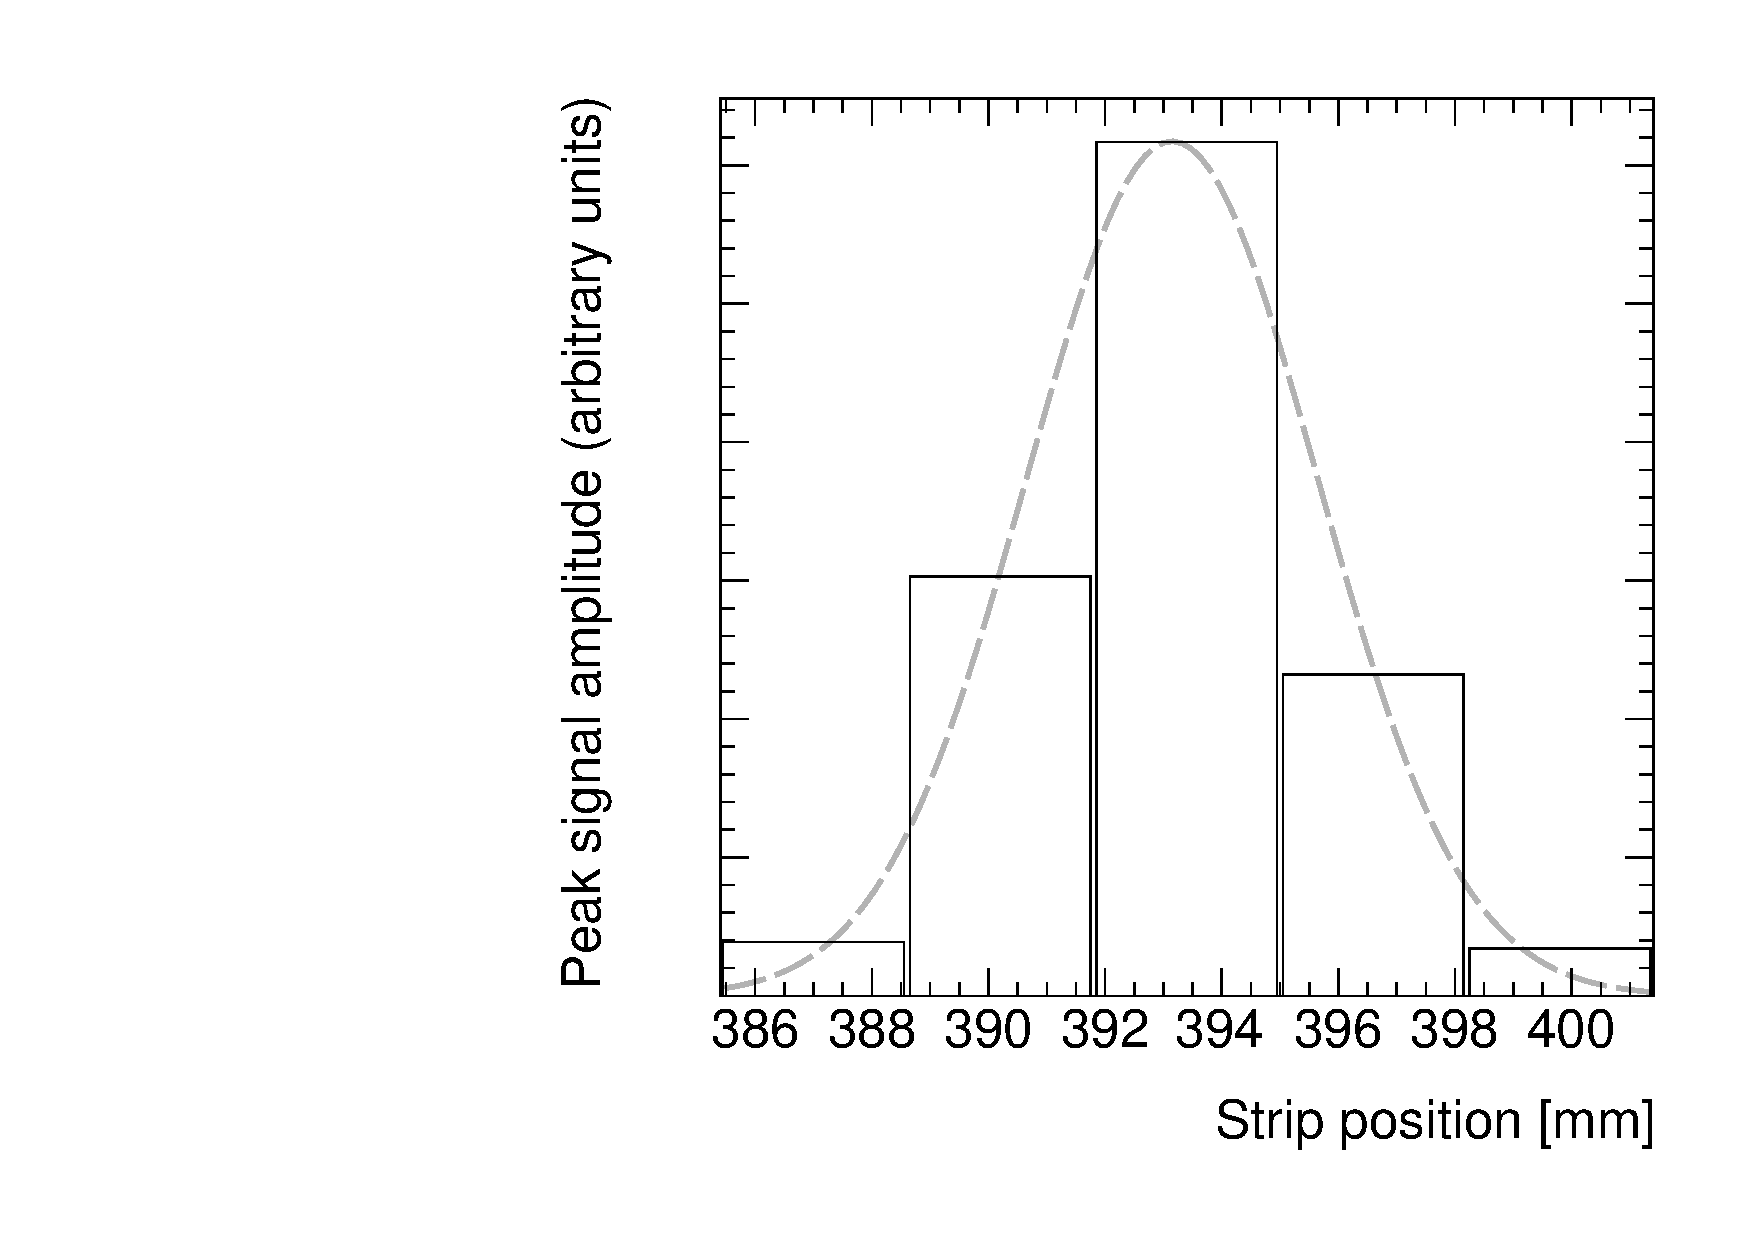
\includegraphics[width = 0.5\textwidth]{figures/sample_cluster_QL2C04_event5_layer2.pdf}
    \caption{A sample cluster resulting from signal recorded on a group of contiguous strips after the passing of a muon. The grey dashed line represents the result of a fit to a Gaussian distribution.}
    \label{fig:sample_cluster}
\end{figure}
\newpage
\restoregeometry

The $y$-coordinate of the muon's position is taken as the Gaussian mean of the peak signal amplitude distribution across a group of contiguous strips that registered hits. The process of grouping contiguous strip hits on a layer is called clustering, and the resulting group is called a cluster. Figure~\ref{fig:mwpc_coords} sketches the clustering process and a sample cluster is shown in Figure~\ref{fig:sample_cluster}. The data acquisition system recorded the identification number of the strip electrode that was hit and in the clustering process the position of the center of the strip electrode is calculated based on the nominal quadruplet geometry. Typically, clusters are built of 3-5 strips. The thickness of the graphite coating over the cathode boards determined how many strips picked up the ionization image charge. Larger clusters can often originate from $\delta$-rays since they spread the ionization charge over a larger area.

Events are removed from further analysis if there are two reconstructed clusters on one sTGC, since some hits could be from electronic noise or a simultaneous second muon traversing the chamber. Clusters are rejected if the cluster size is lesser than three strips (which should not happen for real events thanks to neighbour triggering), and if the cluster size is greater than 25. After all quality selection cuts are applied on hits and clusters, approximately half of the events recorded remain.

The uncertainty on the reconstructed cluster position is assessed by comparing the difference between Gaussian means obtained using two different algorithms. As shown in Appendix~\ref{appendix:clustering}, the difference between the means from the two algorithms considered is found to be approximately \SI{60}{\micro\meter} on average, larger than the statistical uncertainty on the Gaussian mean obtained from the cluster fit. Therefore, an uncertainty of \SI{60}{\micro\meter} is assigned to the reconstructed y-coordinate of a muon. 

The reconstructed $x$ and $y$ coordinates on each quadruplet layer are used to reconstruct a straight track, independently, in the $x$-$z$ and $y$-$z$ planes. Tracks are reconstructed using muon coordinates for every possible pair of two sTGC layers.  For example, if an event has muon coordinates reconstructed on all four layers, a total of six track segments in the $x$-$z$ plane and six track segments in the $y$-$z$ plane will be reconstructed. 

%TODO : Include hit and track map? - yes if Brigitte says you need a num_entries plot in chapter 3. You didn't include it because you never mention wire supports in TH2 analysis. But if you want to add num entries for clarity, include cluster map here. Cluster map > raw hits because less cuts and gets across the idea that x is just hit or no hit while y comes from clustering.  

% Edit count: Lia - 2, Brigitte - 0

% --------------------------------------------------
\section{Relative local offsets}
% --------------------------------------------------

The offset of a strip from its nominal position can be modeled as a passive transformation. The \textit{local offset} is defined as the shift in the strip pattern with respect to nominal geometry in a specific area of the sTGC. Local offsets systematically change the set of strips nearest to muons passing through an area. The data preparation software assumes that strips are in their nominal positions, so the recorded $y$-coordinate of the muon on layer $i$, $y_i$, is shifted opposite to the layer's local offset, $d_{local, i}$, by
% Maybe useful sentence?: The local offset is a result of the non-conformities in the strip pattern etching and inter-layer misalignments.
\begin{equation}
    y_i = y_{nom, i} - d_{local, i},
    \label{eqn:local_translation}
\end{equation}
% Maybe useful sentence?: The true position of individual cosmic muons is not known, and in the analysis the four detector planes float with respect to a software-implemented origin that is not associated with a fixed physical location.
where $y_{nom, i}$ is the position of the muon that would have been recorded on layer $i$ if there was no local offset. Equation~\ref{eqn:local_translation} ignores other factors that affect the cluster position, like position resolution. With cosmics data, there was no external reference to measure $y_{nom, i}$ and the local offset is unknown. Therefore, only {\em relative} local offsets can be measured. 

% Potential BREAK for Motivation section at beginning ^
To measure relative local offsets, two of the four sTGC layers are chosen to provide a reference coordinate system. Relative local offsets are calculated with respect to the two reference or fixed layers. The hits on the two fixed layers were used to create tracks that can be interpolated or extrapolated (polated) to the other two layers. The set of two fixed layers and the layer polated to are referred to as a tracking combination. The residual of track $i$, $\Delta_i$, is defined as,
\begin{equation}
    \Delta_i = y_{i} - y_{track, i},
    \label{eqn:residual}
\end{equation}

where $y_{track, i}$ is the polated track position on the sTGC layer the residual is measured on. Track residuals are affected by the local offset in the area of each layer's hit. As an example, in Figure~\ref{fig:fake_event_display}, the residual on layer 2 perhaps indicates that layer 2 is offset with respect to layers 1 and 4 in the area of the track. Of course, a single track residual says nothing of the real relative local offset because of the limited spatial resolution of the detectors and fake tracks caused by noise or delta rays. However, the mean of residuals for all tracks in a region of interest will be shifted systematically by the local offsets between layers~\cite{lefebvre_thesis}. For a quadruplet with nominal geometry, the mean of residuals should be zero in all regions and for all reference frames, unlike the example regions in Figure~\ref{fig:res_dist}. The value of the mean of residuals is a measure of the relative local offset of the layer with respect to the two fixed layers used to reconstruct the muon track. The sign convention is such that the mean of residuals is opposite to the relative local offset.

\begin{figure}
    \centering
    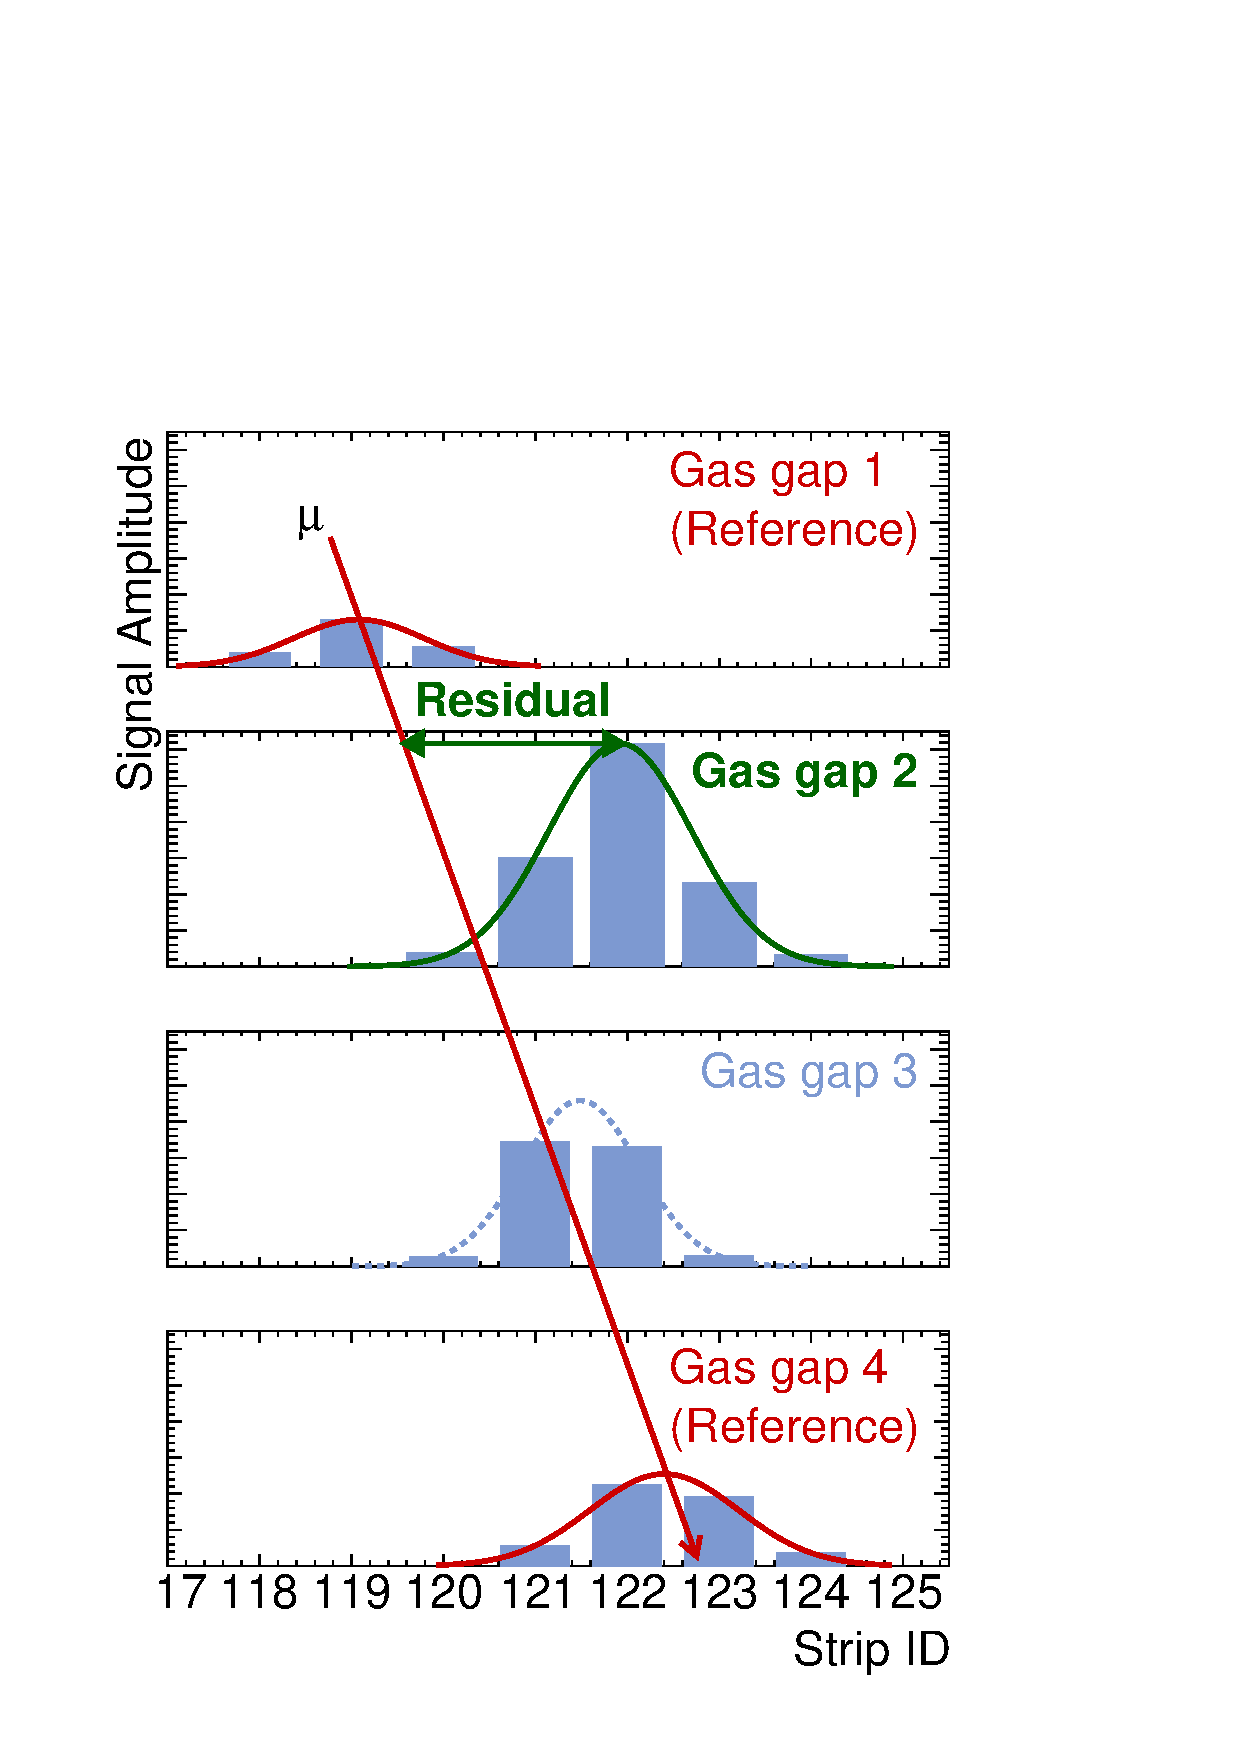
\includegraphics[width = \textwidth]{figures/figure_fake_event_display.pdf}
    \caption{Representation of a muon event recorded by an sTGC quadruplet. The charge clusters measured using strip electrodes are fit with a Gaussian distribution and the fitted mean is taken as the reconstructed muon position. A track is built from the chosen reference layers, 1 and 4, and the track residual is calculated on layer 2. The clusters come from a real muon, but their positions were modified to highlight the non-zero value of the residual on layer 2.}
    \label{fig:fake_event_display}
\end{figure}

\begin{figure}
\centering
\begin{subfigure}{.5\textwidth}
  \centering
  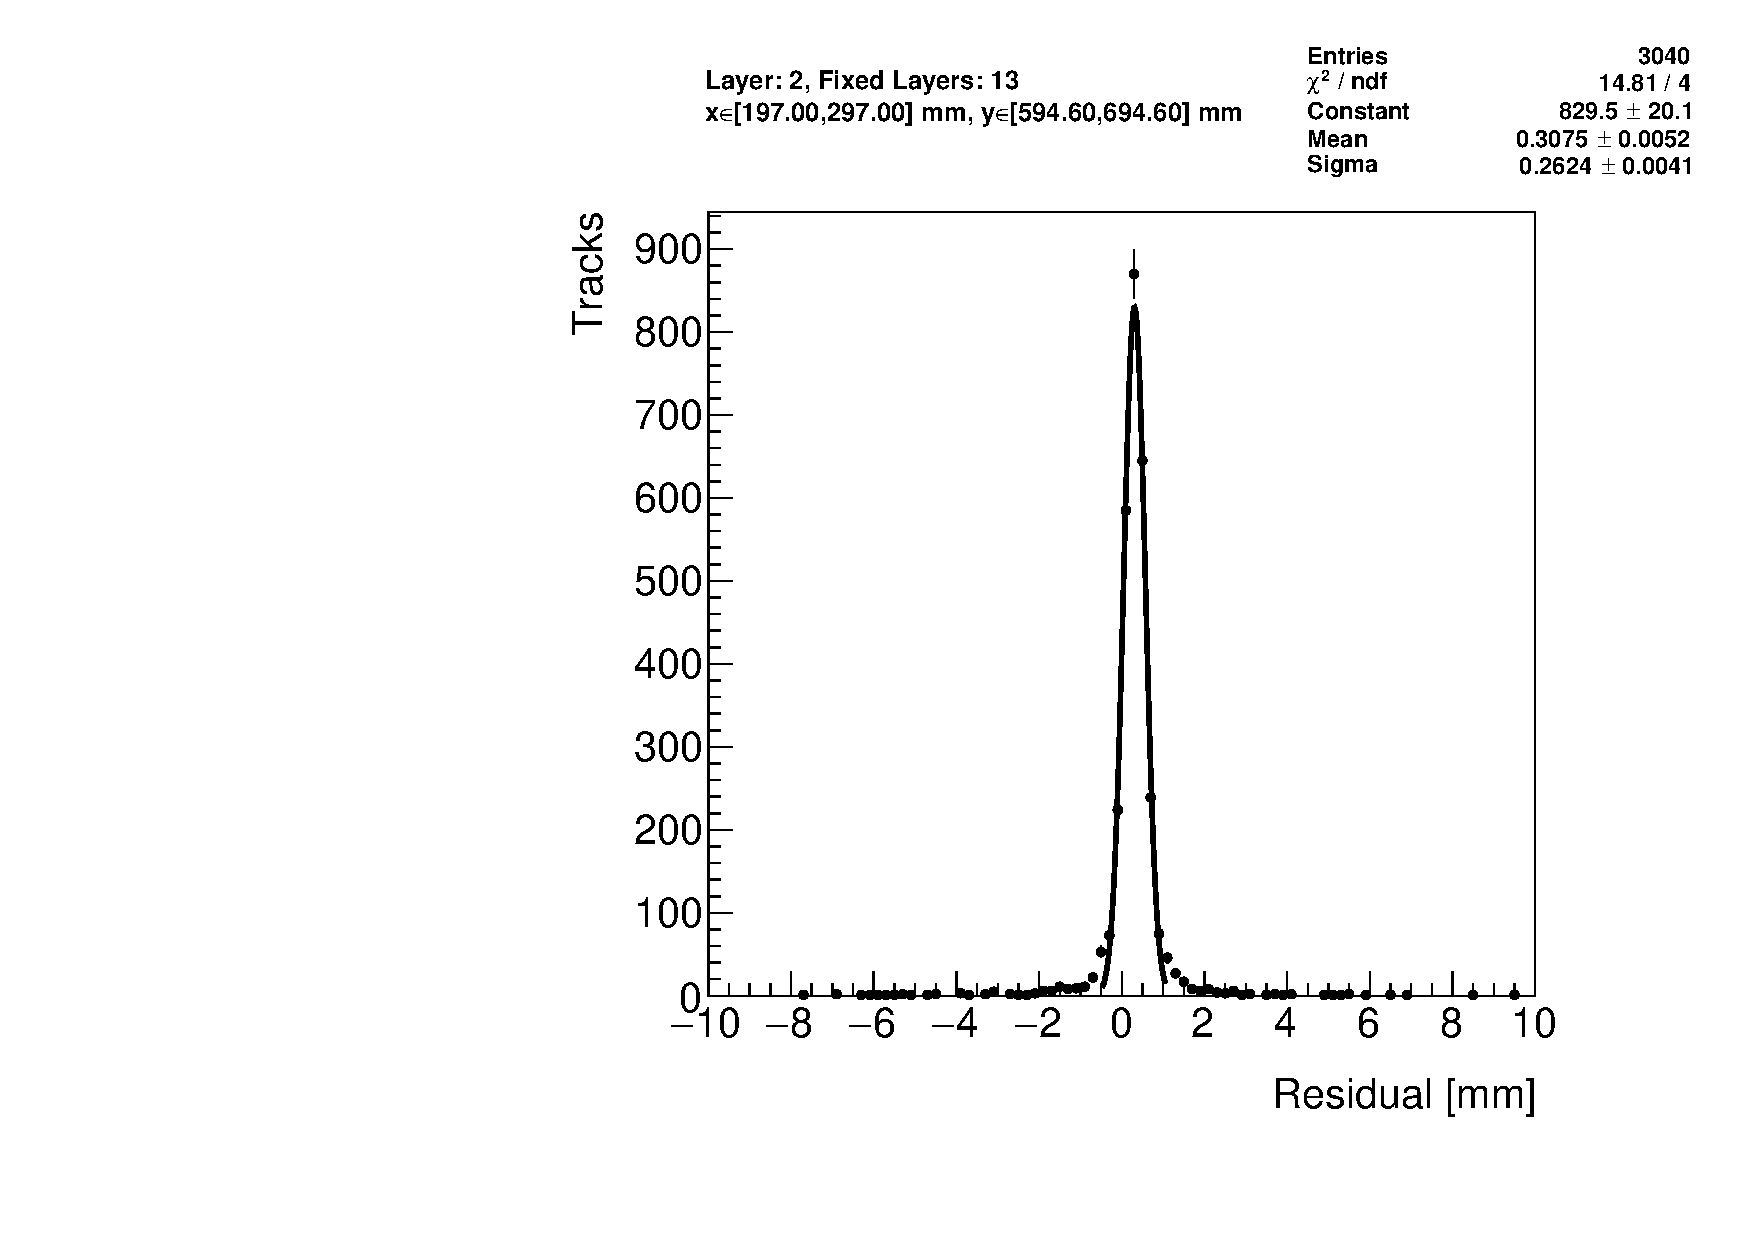
\includegraphics[width=\linewidth]{figures/figure_res_dist_QL2P11_3100V_2021-08-05_xbin_12_ybin_7_layer2_fixedlayers13.pdf}
  \caption{Tracks on layer 2, reference layers 1 and 3.}
  \label{fig:res_dist_L2_F13}
\end{subfigure}
\begin{subfigure}{.5\textwidth}
  \centering
  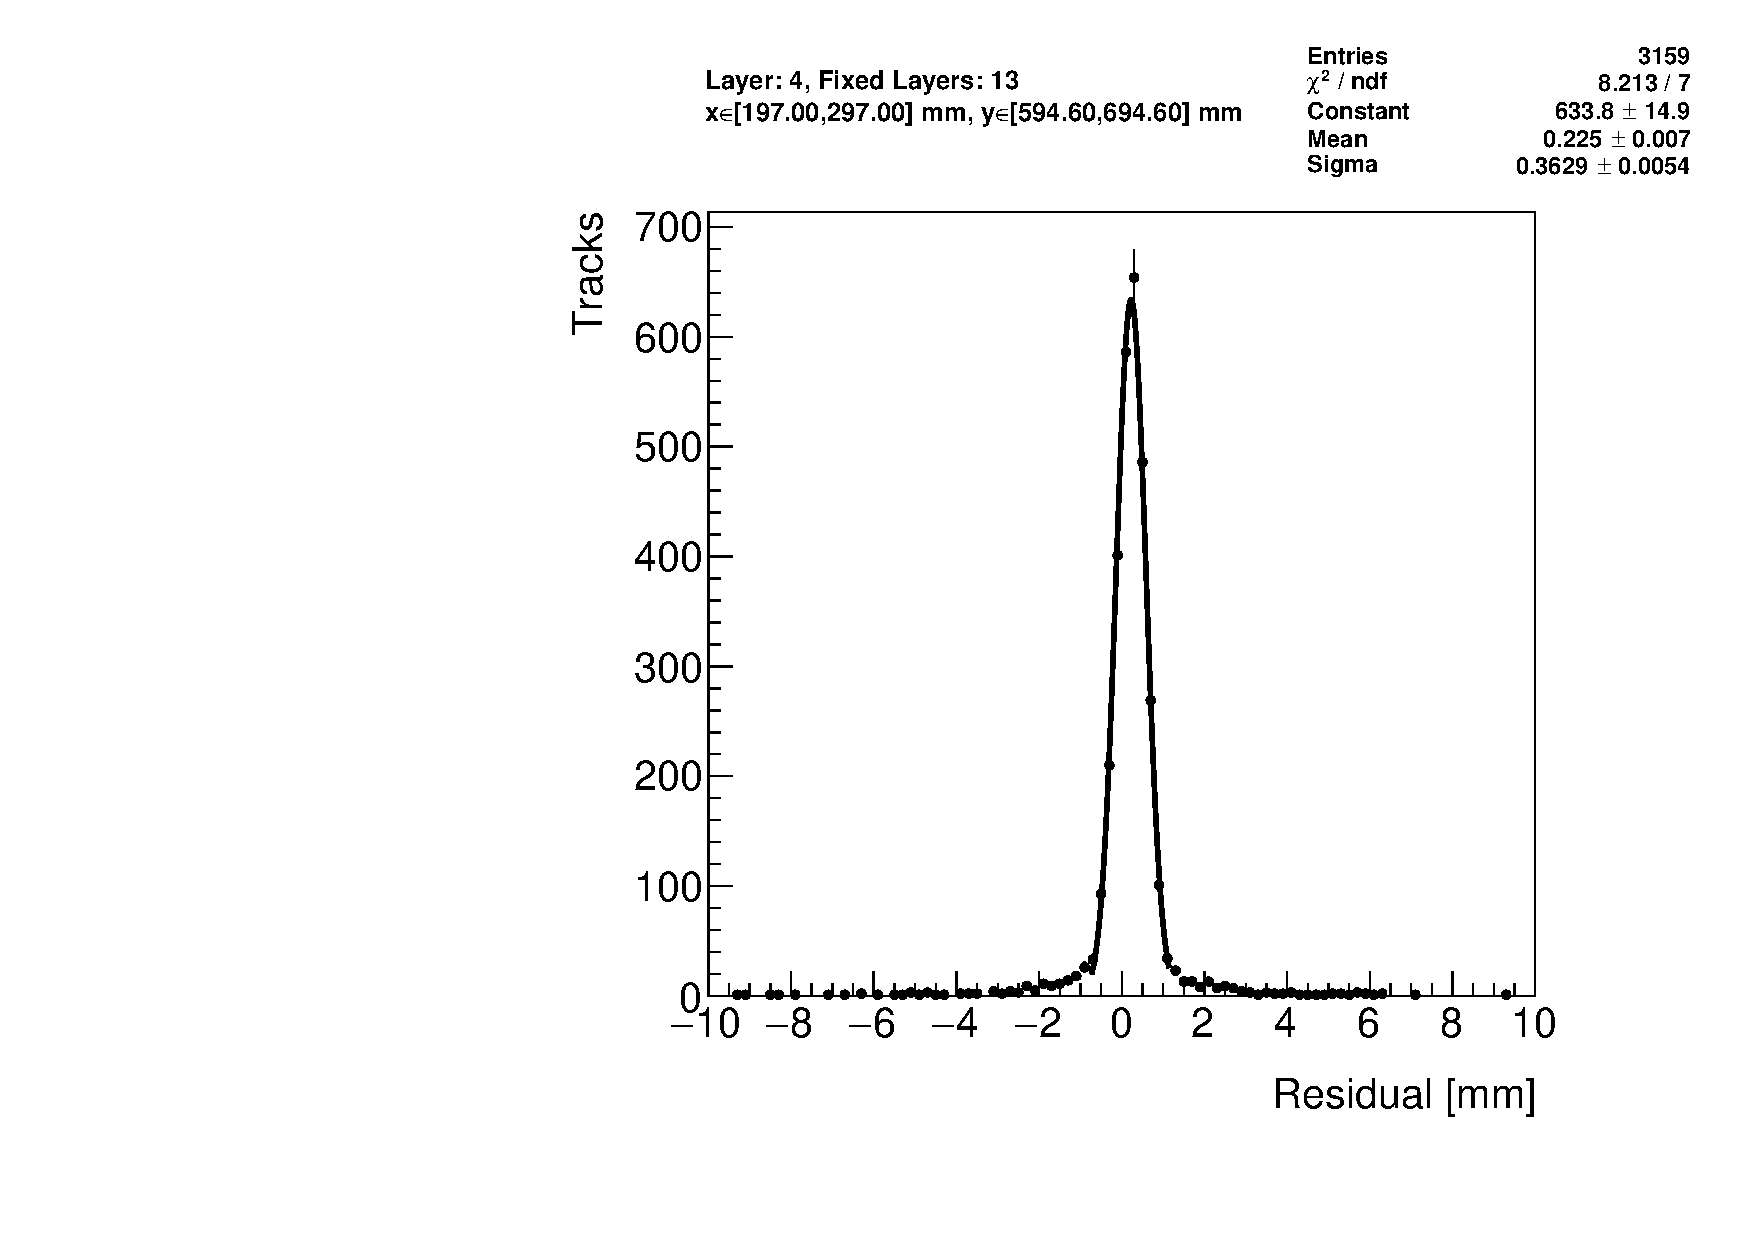
\includegraphics[width=\linewidth]{figures/figure_res_dist_QL2P11_3100V_2021-08-05_xbin_12_ybin_7_layer4_fixedlayers13.pdf}
  \caption{Tracks on layer 4, reference layers 1 and 3.}
  \label{fig:res_dist_L4_F13}
\end{subfigure}
\caption{Residual distribution in the region $x\in\left[197, 297\right]$~mm,  $y\in\left[594.6, 694.6\right]$~mm (\SI{100}{mm} by \SI{100}{mm} area) for two different tracking combinations. Data from quadruplet QL2.P.11.}
\label{fig:res_dist}
\end{figure}

To study the relative local offsets, residual distributions across each strip layer of a quadruplet for all possible tracking combinations are assembled and fitted. As expected, the residual distributions are wider for tracking combinations where the extrapolation lever arm is largest, as in the example distributions shown in Figure~\ref{fig:res_dist}. In general, residual means from distributions of residuals with geometrically less favourable tracking combinations have larger statistical and systematic uncertainties. The bin size of \SI{200}{\micro\meter} for the distributions shown in Figure~\ref{fig:res_dist} was chosen based on the uncertainty on residuals calculated from tracks on layer 4 (1) built from hits on layers 1 and 2 (3 and 4) given a cluster $y$-coordinate uncertainty of \SI{60}{\micro\meter} (discussed in Section~\ref{subsec:clustering} and Appendix~\ref{appendix:clustering}), since these tracks yield residuals with the largest uncertainties.

A Gaussian fit is used to extract the mean of the residual distributions. The residual distributions are actually better modeled by a double Gaussian distribution, which better captures the distribution tails in Figure~\ref{fig:res_dist}. However, a study described in Appendix~\ref{appendix:systematics_res_fit_fcn} found that a fit to a single Gaussian function in the core of the distribution is sufficient to reconstruct the mean of the distribution.

The area of the region of interest where tracks residuals were included in the residual distribution was \SI{100}{\milli\meter} by \SI{100}{\milli\meter}. The size balanced the number of tracks falling in the region of interest to give a small statistical uncertainty on the fitted mean while being smaller than the order on which local offsets were expected to change significantly. ``Significantly'' was defined as \SI{100}{\micro\meter}, the required position resolution of the sTGCs and the precision to which strip positions should be known. The distance over which local offsets are expected to change significantly can be estimated using a simple alignment model. Assuming the strips of a layer have been displaced uniformly from their nominal positions by a global offset and rotation, the distance in $x$ that a large but possible rotation of \SI{1}{mrad} changes the local offset by \SI{100}{\micro\meter} is \SI{100}{mm}.

% Original position of this paragraph
% It is only possible to calculate relative local offsets with cosmics data because there was no external reference to measure positions on all layers with respect to. As an example, assuming that the residual on layer 2 in figure~\ref{fig:fake_event_display} is representative of the relative local offset, the residual on layer 2 could be caused by the strips on layer 2 being misaligned from nominal, but it could also be caused by strips on layers 1 and 4 being misaligned from nominal while the strips on layer 2 are in their nominal positions! Any number of combinations of local offsets on layers 1, 2 and 4 could produce the residual on layer 2. The value of relative local offset measurements will be shown and discussed throughout this work.
The means of residuals are plotted across each sTGC layer for every possible tracking combination to get a picture of the how the relative local offsets change as a function of position over the layer's surface. Figure~\ref{fig:res_mean_th2} shows the mean of residuals on layer 2 calculated with layers 1 and 3 as reference for two different quadruplets, referred to as QL2.P.11 and QL2.P.8. In Figure~\ref{fig:res_mean_th2_ql2p11}, the Gaussian mean of the residual distribution in Figure~\ref{fig:res_dist_L2_F13} is the entry in the bin defined by the  boundaries $x\in\left[197, 297\right]$~mm,  $y\in\left[594.6, 694.6\right]$~mm.

Many of the residual means are non-zero and change smoothly over layer 2, indicating that there are relative local offsets stemming from global misalignments between the strip patterns of different sTGC layers in both quadruplets. Given that the residual mean changes with $x$ in Figure~\ref{fig:res_mean_th2_ql2p11}, quadruplet QL2.P.11 likely has a rotation of layer 2 with respect to layers 1 and 3, combined with an offset of the entire layer. The residual means are smaller in Figure~\ref{fig:res_mean_th2_ql2p8} indicating that quadruplet QL2.P.8 is less misaligned overall than QL2.P.11; however, the relative local offsets range between $\pm$\SI{200}{\micro\meter} so they are significant enough to warrant a correction so the quadruplet can achieve the required track angular resolution in the NSW.

\newpage
\thispagestyle{empty}
\newgeometry{top=0.5in,bottom=0.5in}
\begin{figure}
\centering
\begin{subfigure}{\textwidth}
  \centering
  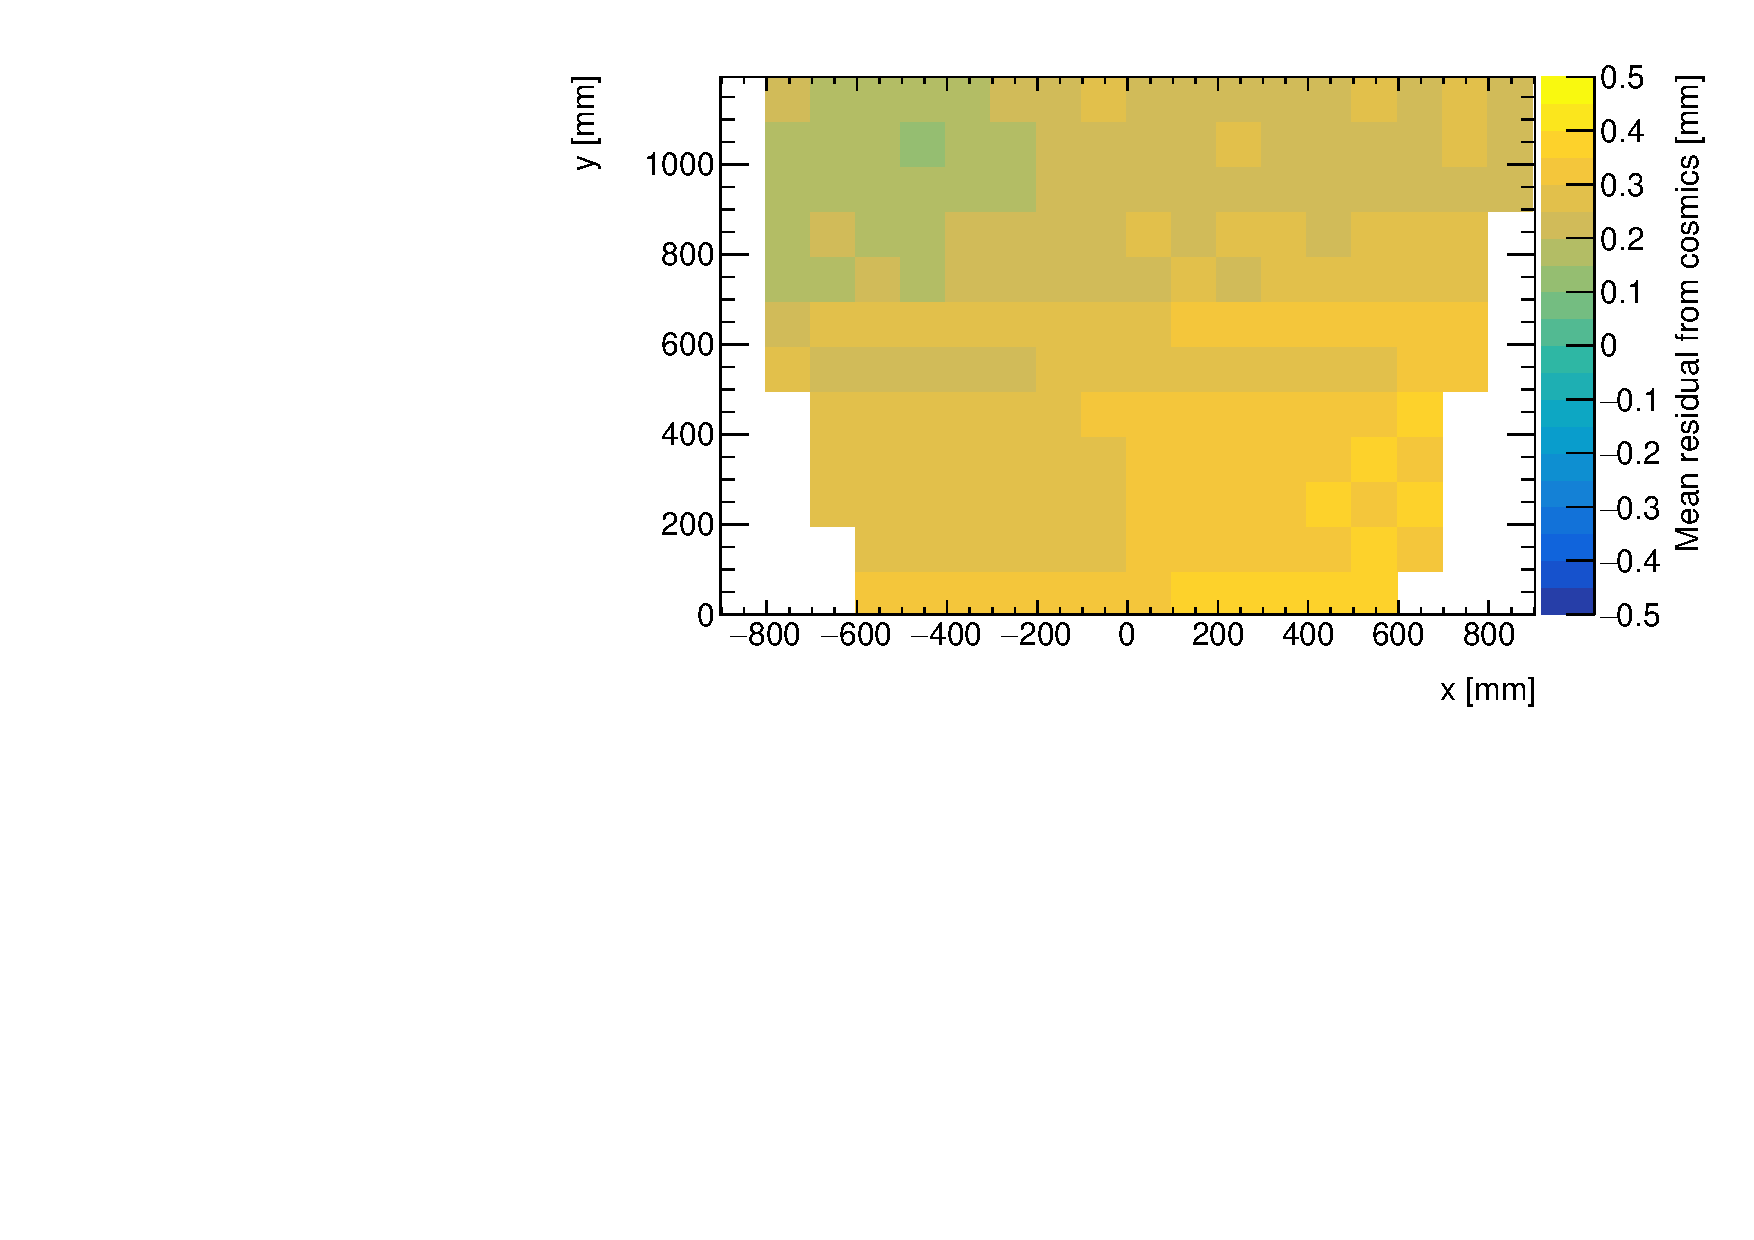
\includegraphics[width=\linewidth]{figures/figure_QL2P11_3100V_2021-08-05_th2_means_layer2_fixedlayers13.pdf}
  \caption{Mean of track residuals on layer 2, obtained using layers 1 and 3 as reference, for QL2.P.11.}
  \label{fig:res_mean_th2_ql2p11}
\end{subfigure}%
\vspace*{\floatsep}
\begin{subfigure}{\textwidth}
  \centering
  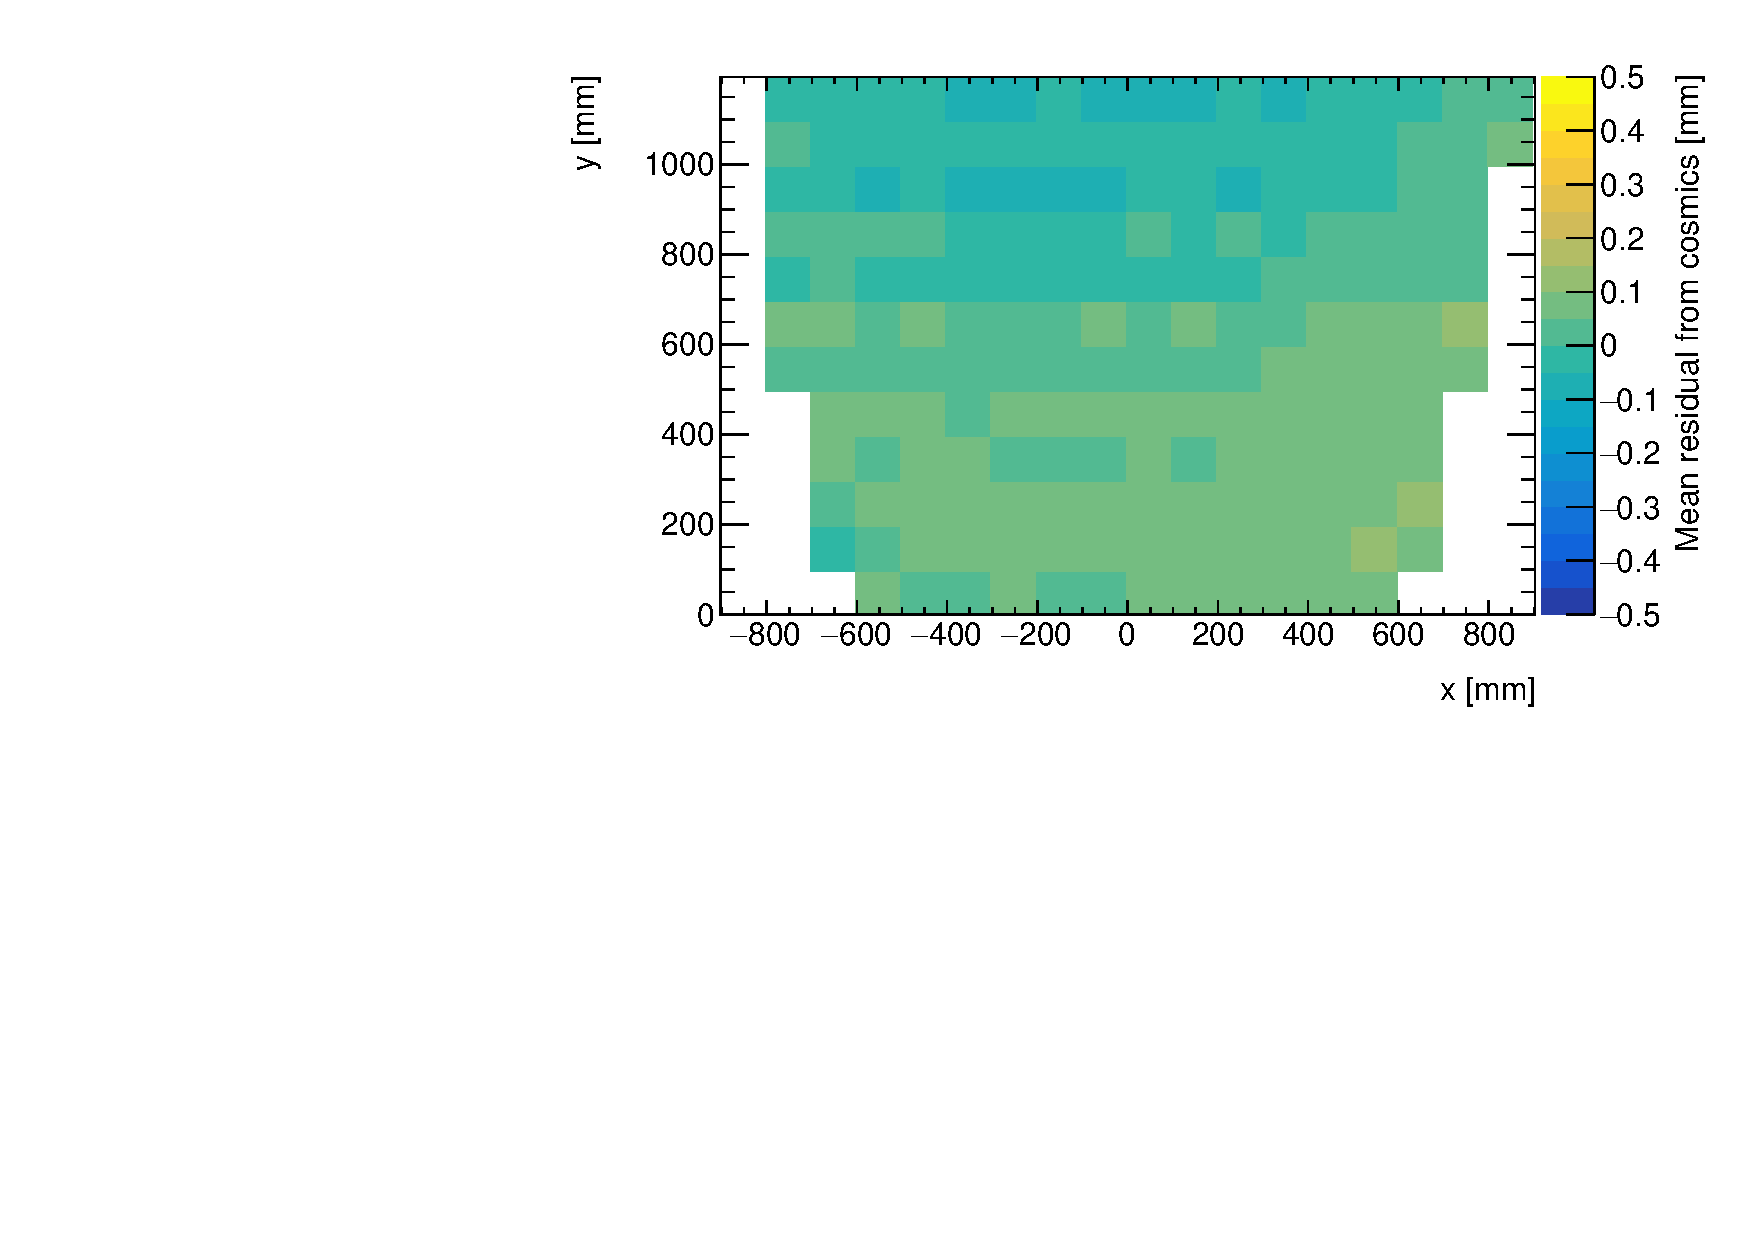
\includegraphics[width=\linewidth]{figures/figure_QL2P08_3100V_2021-08-03_th2_means_layer2_fixedlayers13.pdf}
  \caption{Mean of track residuals on layer 2, obtained using layers 1 and 3 as reference, for QL2.P.8.}
  \label{fig:res_mean_th2_ql2p8}
\end{subfigure}
\caption{Mean of residuals in each \SI{100}{\milli\meter} by \SI{100}{\milli\meter} bin over the area of sTGC layer 2 for quadruplets QL2.P.11 and QL2.P.8. The entry in $x\in\left[197, 297\right]$~mm,  $y\in\left[594.6, 694.6\right]$~mm of Figure~\ref{fig:res_mean_th2_ql2p11} corresponds to the fitted Gaussian mean in Figures~\ref{fig:res_dist_L2_F13}. The mean of residuals has the same value and opposite sign to the relative local offset of layer 2 with respect to the reference frame defined by layers 1 and 3.}
\label{fig:res_mean_th2}
\end{figure}
\newpage
\restoregeometry

% --------------------------------------------------
\section{Systematic uncertainty}
% --------------------------------------------------
\label{sec:cosmics_sys_uncerts}

The statistical uncertainty on the local residual means was typically around \SI{10}{} - \SI{20}{\micro\meter}, and Appendix~\ref{appendix:statistics} shows that the analysis is not statistically limited by the number of triggers collected for each quadruplet. Systematic uncertainties were found to be larger than the statistical uncertainty on the residual means.

Several analysis choices had some degree of impact on the fitted means of local track residual distributions. To study the impacts, the residual means were calculated in different ways and distributions of the differences made. The complete studies are shown in Appendix~\ref{appendix:systematics}. The root-mean-square (RMS) of the residual mean difference distributions were used to quantify the impact of the different analysis choices as systematic uncertainties on the residual means. The following analysis choices are considered:
\begin{itemize}
  \item The impact of performing a single or double Gaussian fit on the track residual distributions is studied. As shown in Appendix~\ref{appendix:systematics_res_fit_fcn}, the difference between fitting the track residual distribution with a single or double Gaussian function varies between 10-\SI{30}{\micro\meter} from the most to least geometrically favourable tracking combinations.
  \item The impact of the operating voltage used during data taking is investigated. Cosmic muon data was recorded at \SI{2.9}{kV} and \SI{3.1}{kV}. As described in Appendix~\ref{appendix:systematics_2900V_vs_3100V}, an uncertainty between 10-\SI{40}{\micro\meter} is assigned to the different tracking combinations.
  \item The impact of using different Gaussian fitting algorithms used to reconstruct the position of a charge cluster was considered. Clusters are fit with the Minuit2~\cite{hatlo_developments_2005} and Guo's method~\cite{guo_simple_2011}. As shown in Appendix~\ref{appendix:systematics_cluster_fit_fcn}, the resulting difference in residual means is between 10-\SI{30}{\micro\meter} from the most to least geometrically favourable tracking combinations.
  \item The impact of correcting reconstructed cluster positions for differential non-linearity (DNL) is studied. DNL is fully described in Appendix~\ref{appendix:systematics_dnl}. It is a bias in the reconstructed cluster position that comes from discretely sampling a continuous distribution, in this case the charge distribution~\cite{endo_systematic_1981, lefebvre_thesis, abusleme_performance_2016}. The difference between residual means is compared with and without correcting the reconstructed cluster positions. Appendix~\ref{appendix:systematics_dnl} shows that the impact of the correction is smaller than \SI{10}{\micro\meter} for all tracking combinations, which is almost negligible.
\end{itemize}
%The differences in fitted local residual means when calculated in different ways were studied in detail in appendix~\ref{appendix:systematics}. Systematic uncertainties are assigned per tracking combination as the root-mean-square (RMS) of the distribution of the difference in residual means. For example, the RMS associated with fitting the local residual distributions with a Gaussian or double Gaussian is \SI{25}{\micro\meter} for the geometrically least favourable tracking combinations. The distribution is shown in appendix~\ref{appendix:systematics_res_fit_fcn}. For geometrically similar tracking combinations (like: tracks on layer 1 built from hits on layers 3 and 4, and tracks on layer 4 built from hits on layers 1 and 2), the systematic uncertainty was assigned as the average RMS of both.

%Other choices were: whether to use data collected at \SI{2.9}{kV} or \SI{3.1}{kV} (both are collected at McGill); what cluster fitting algorithm to use; and whether or not to apply a differential non-linearity (DNL) correction to the cluster $y$-positions~\cite{abusleme_performance_2016}. A systematic uncertainty was assigned using the method above to account for the effect of each choice and quantify the robustness of the mean of residuals. The reasons for each choice are listed below.

%Data taken at \SI{3.1}{kV} was used over \SI{2.9}{kV} because the strip and wire tracking efficiency increases with higher voltage~\cite{lefebvre_thesis} (appendix~\ref{appendix:systematics_2900V_vs_3100V}).

%The \package{Minuit2} package~\cite{hatlo_developments_2005} was used to fit clusters over Guo's method~\cite{guo_simple_2011} because it provided automatic statistical uncertainty estimates and is the standard fit algorithm of \package{ROOT}~\cite{ROOT_paper} (appendix~\ref{appendix:systematics_cluster_fit_fcn}).

%The DNL correction was not applied because its effect on the residual means was negligible (appendix~\ref{appendix:systematics_dnl}).

A summary of the systematic uncertainties assigned to the local means of residuals for each tracking combination is given in Table~\ref{tab:sys_uncerts}. The RMS of the distributions of residual mean differences of geometrically similar tracking combinations are averaged and the average value is taken as the systematic uncertainty for those tracking combinations. An example of a geometrically similar pair of tracking combinations is fixing layers 1 and 2 and extrapolating to layer 3 or fixing layers 2 and 3 and extrapolating to layer 4; geometrically similar combinations have the same polation lever arm. The total systematic uncertainty is obtained by summing in quadrature all the different sources of systematic uncertainty. The uncertainty in each mean of residuals is obtained by summing in quadrature the statistical uncertainty in the mean of residuals and the appropriate systematic uncertainty for the tracking combination used to calculate the mean of residuals.

% OR
%The following were treated as sources of systematic uncertainty:
%\begin{itemize}
 % \item The impact of performing a single- or double-Gaussian fit on the track residual distributions (appendix~\ref{appendix:systematics_res_fit_fcn})
 % \item The impact of the operating voltage used during data taking, since cosmics data was recorded at both \SI{2.9}{kV} and \SI{3.1}{kV}. As shown in appendix~\ref{appendix:systematics_2900V_vs_3100V}, the RMS of the difference in fitted track residual means varies between 10-\SI{40}{\micro\meter} from the most to least geometrically favourable tracking combinations.
%\end{itemize}
\begin{table}

\begin{tabularx}{\textwidth} {
 | >{\raggedright\arraybackslash}X
 | >{\raggedright\arraybackslash}X 
 | >{\raggedright\arraybackslash}X 
 | >{\raggedright\arraybackslash}X 
 | >{\raggedright\arraybackslash}X 
 | >{\raggedright\arraybackslash}X 
 | >{\raggedright\arraybackslash}X | }
 
 \hline
 \textbf{Tracking geometry} & \textbf{Residual distribution fit function (\ref{appendix:systematics_res_fit_fcn})} & \textbf{Cosmics data collection voltage (\ref{appendix:systematics_2900V_vs_3100V})} & \textbf{Cluster fit algorithm (\ref{appendix:systematics_cluster_fit_fcn})} & \textbf{Apply DNL correction or not (\ref{appendix:systematics_dnl})} & \textbf{Total} \\ 
 \hline
 \hline 
   Similar to layer 3, fixed layers 1, 2 & 0.01~mm & 0.04~mm & 0.02~mm & 0.01~mm & \textbf{0.05~mm} \\
 \hline
   Similar to layer 4, fixed layers 1, 2 & 0.03~mm & 0.01~mm & 0.03~mm & 0.01~mm & \textbf{0.10~mm} \\
 \hline
    Similar to layer 2, fixed layers 1, 3 & 0.01~mm & 0.02~mm & 0.01~mm & 0.000~mm & \textbf{0.03~mm} \\
 \hline
    Similar to layer 4, fixed layers 1, 3 & 0.01~mm & 0.04~mm & 0.01~mm & 0.01~mm & \textbf{0.04~mm} \\
 \hline
    Similar to layer 2, fixed layers 1, 4 & 0.01~mm & 0.04~mm & 0.01~mm & 0.01~mm & \textbf{0.04~mm} \\
 \hline
 
\end{tabularx}
\caption{Systematic uncertainties assigned for each analysis option per tracking combination. Details can be found in Appendix~\ref{appendix:systematics}. The total systematic uncertainty is obtained by summing in quadrature all the individual systematic uncertainties.}
\label{tab:sys_uncerts}
\end{table}

% --------------------------------------------------
\section{Discussion}
% --------------------------------------------------

The total uncertainty in the residual means, and hence the relative local offsets, is typically less than the design sTGC position resolution of $\sim$\SI{100}{\micro\meter}~\cite{nsw_tdr}. Therefore, the residual means are relevant input for alignment studies.

The relative local offsets calculated from the means of residual distributions over the surface of an sTGC layer for all tracking combinations provide a complete picture of the relative alignment between sTGC layers in a quadruplet module. In fact, cosmic muon testing is the only characterization technique where the entire surface of quadruplet layers can be probed since muons hits are distributed almost uniformly; the CMM~\cite{carlson_results_2019} and x-ray methods~\cite{lefebvre_precision_2020} depend on measurements at reference points, and test beams only have a limited beam spot to work with~\cite{abusleme_performance_2016}. By looking at 2D-histograms of residual means like Figure~\ref{fig:res_mean_th2} for all tracking combinations, it is easy to identify quadruplets that suffer large relative misalignment since many residual means differ significantly from zero. Moreover, the pattern in the residual means can be used to motivate a physical interpretation of misalignments. The residual means can be used as a reference, cross check, or input to other alignment studies.

Relative local offsets cannot be used to position strips in the absolute ATLAS coordinate system because there is no external reference to measure positions on all layers with respect to. The lack of an external absolute reference frame means that there is not enough information to unfold relative local offsets into absolute local offsets (with respect to the nominal quadruplet geometry). As an example, assuming that the residual on layer 2 in Figure~\ref{fig:fake_event_display} is representative of the absolute value of the relative local offset, the residual on layer 2 could be caused by the strips on layer 2 being misaligned from nominal, but it could also be caused by strips on layers 1 and 4 being offset from nominal while the strips on layer 2 are in their nominal positions! Any number of combinations of local offsets on layers 1, 2 and 4 could produce the residual on layer 2. Absolute local offsets must be calculated using another method: the x-ray method.

% ==================================================
% CHAPTER 6: Using x-rays to measure relative strip position offsets
% ==================================================

\chapter{Using x-rays to measure relative strip position offsets}
\label{chap:xray}

This chapter describes the analysis of x-ray data to measure relative local strip position offsets, which can be compared with results obtained using cosmic data. The reader is referred to the paper describing the x-ray method~\cite{lefebvre_precision_2020}, although some minor changes to the experimental setup  have been made since it was written. The experimental setup described here is current and was used to collect the data presented in this thesis.
% Makesure to put this in the statement of contribution

% NOTE: Wrote this with information available in JINST, or things I know to be updated (eg. brass holder and collimator). I can guess at other things based on the WedgeAlignment-Production code, but don't actually know. Those things are in iffalse statements.
% --------------------------------------------------
\section{Experimental setup}
% --------------------------------------------------

The x-ray tests were performed after the quadruplets arrived at CERN, were assembled into wedges, and alignment platforms installed. An x-ray gun was attached to one of the alignment platforms glued to the surface of the wedge and the x-ray beam profile was recorded by the strip electrodes.

\begin{figure}[t]
    \centering
    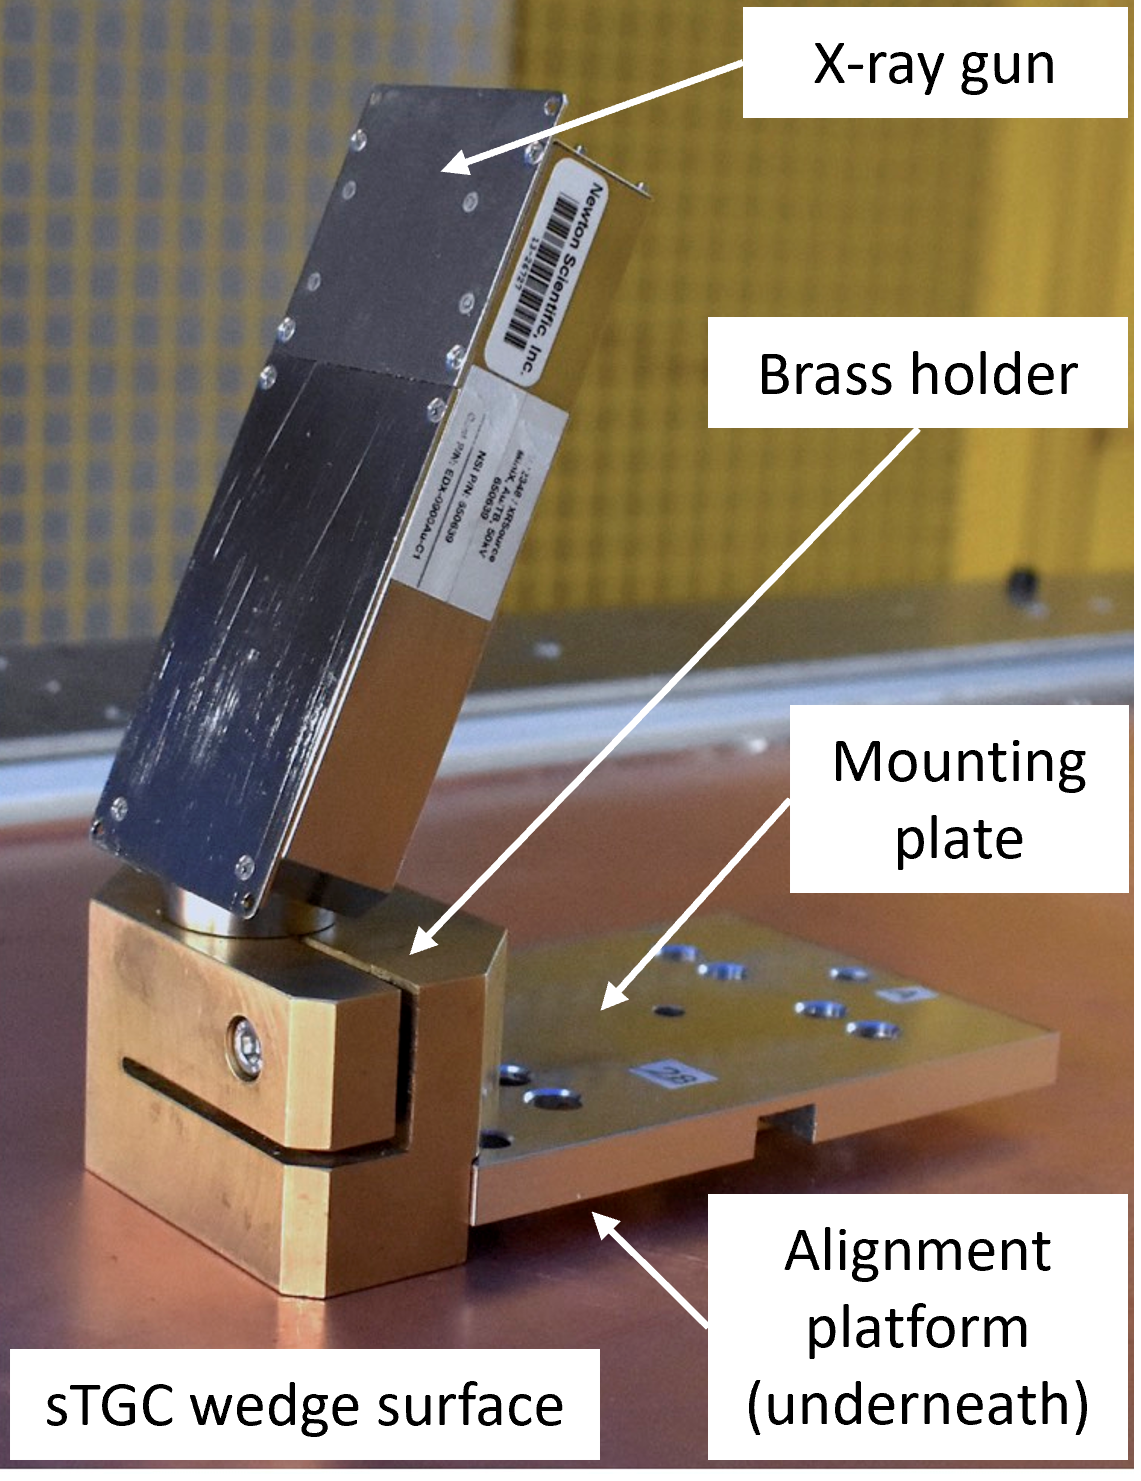
\includegraphics[width = 0.5\textwidth]{figures/xray_setup.png}
    \caption{The x-ray gun mounted to an alignment platform on the surface of the a sTGC wedge. Adapted from~\cite{lefebvre_precision_2020}.}
    \label{fig:xray_setup}
\end{figure}

The sTGC wedges were installed on carts that could rotate their surface to a horizontal position. A mounting platform was installed on top of the alignment platform using a three-ball mount. The x-ray gun used was an Amptek Mini-X tube~\cite{xray_gun}. The x-ray gun was placed in a brass holder with built-in \SI{2}{mm} collimator and \SI{280}{\micro\meter} copper filter. The holder was mounted on one of five positions on the mounting platform, as shown in figure~\ref{fig:xray_setup}. The x-ray gun positions were chosen to avoid wire support structures in the sTGCs that reduce hit efficiency~\cite{lefebvre_thesis} and boundaries between sets of strips read out by two different ASICs that could each have different thresholds. 

As with cosmics data collection, each sTGC also needed gas and high voltage to operate. Each sTGC layer was operated at \SI{2.925}{kV} with high voltage from a NIM crate. The sTGC gas volumes were flushed with CO$_2$ before and during data collection. The sTGCs were not operated using the nominal pentane-CO$_2$ gas mixture due to constraints in its availability based on safety concerns. The sTGC efficiency is significantly lower when operated with only CO$_2$.

% The copper filter helped to reduce the effect of attenuation non-uniformities.
The gun produced x-rays with energies under \SI{40}{\kilo\electronvolt} with peaks in the 7-\SI{15}{keV} range. Peaks in the 0-\SI{30}{keV} range were filtered out by the copper filter and the copper of the sTGCs. The x-rays mostly interacted with the sTGC wedge's copper electrodes and gold-plated tungsten wires via the photoelectric effect. The resulting photoelectrons that enter the gas volume caused ionization avalanches that were picked up by the readout strips.
% During ATLAS operation, the position of the source plates will be monitored using the new alignment system~\cite{nsw_tdr}. Therefore, their position will be known in the absolute ATLAS coordinate system. 

% --------------------------------------------------
\section{Data acquisition}
% --------------------------------------------------

A different version of the same front end electronics, but the same ASIC, as used in cosmics testing were used for the x-ray testing to measure the peak signal amplitude. Data was collected for two minutes per gun position with random triggers. A trigger recorded all signals above threshold. \iffalse within \SI{75}{ns} and the signals on neighbouring strips.\fi  Pad and wire data was not recorded.
% Neighbour triggering based on my understanding of the analysis. Does not actually matter for these purposes.

% --------------------------------------------------
\section{Data preparation}
% --------------------------------------------------

Following a similar approach to the cosmics data analysis described in chapter~\ref{chap:cosmics}, a default pedestal is subtracted from the signal peak amplitude on each electrode.

Clusters are defined as groups of contiguous strip hits recorded within \SI{75}{ns}. The distribution of peak signal amplitude from continuous strip hits is fitted with a Gaussian function, and the mean of the fitted Gaussian is taken as the cluster position. Cluster positions are corrected for DNL (see definition in appendix~\ref{appendix:systematics_dnl}). Although the impact of the DNL correction is small on the reconstructed cluster means, it is important to improve the spatial resolution of the reconstructed cluster means. Only clusters composed of hits on 3-5 strips are used in the x-ray analysis. Clusters with signal on more than 5 strips are cut because they were most likely caused by photoelectrons ejected with enough energy to cause more primary ionization and subsequent avalanches as $\delta$-rays.

The x-ray analysis diverges entirely from the cosmics analysis algorithm here because the ionization from x-rays does not originate from one charged particle traversing all layers of a sTGC quadruplet, so there is no track to rebuild. Rather, ionization avalanches~\cite{townsend_electricity_1915} are generated by photoelectrons liberated from the metals of the sTGCs, which only travel through one gas volume and are produced at all angles. Instead of reconstructing a straight line trajectory through multiple sTGC layers, the cluster position distribution on each sTGC layer is used to reconstruct the beam profile. A typical beam profile is shown in figure~\ref{fig:xray_beam_profile}.

\begin{figure}[t]
    \centering
    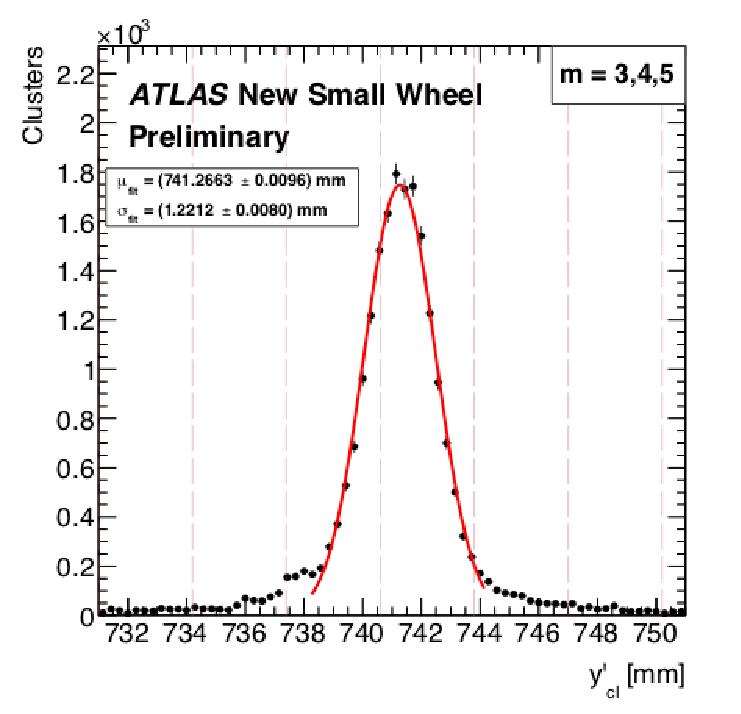
\includegraphics[width = 0.5\textwidth]{figures/figure_xray_beam_profile.pdf}
    \caption{An example distribution of x-ray cluster mean positions after the analysis selection cuts and DNL corrections are applied. The strip cluster multiplicity, $m$, was limited to 3, 4 or 5. The red curve is a Gaussian fit of the distribution and the pink dashed lines denote the edges of the strips~\cite{lefebvre_precision_2020}.}
    \label{fig:xray_beam_profile}
\end{figure}

% --------------------------------------------------
\section{Measuring local offsets}
% --------------------------------------------------
The fitted Gaussian mean of the cluster position distribution is taken as the reconstructed center of the x-ray beam profile on each sTGC layer. The reconstructed center is compared to the expected beam profile center, calculated in two steps. First, the position of the alignment platform with respect to the brass inserts and the nominal position of the strips under the gun position with respect to the brass inserts are used to calculate the expected beam profile center assuming a nominal quadruplet geometry. Second, the expected beam profile center is corrected for the geometry of the brass holder, the positioning and angle of the alignment platforms, and the beam angle. The difference between the expected and reconstructed beam profile centers is a measure of the local offset of the strip electrode pattern. Applying the logic of equation~\ref{eqn:local_translation} to the beam profile, the Gaussian mean of cluster positions on the given layer acts as the recorded position, $y_i$, the expected center is $y_{nom, i}$ and the local offset is $d_{local, i}$ as before, where $i$ denotes the layer. Since the position of the alignment platforms will be monitored continuously by the alignment system in ATLAS~\cite{nsw_tdr}, the position of the strips that should have been at the x-ray gun position are shifted by $d_{local, i}$ and so their absolute positions are known in the ATLAS coordinate system for every position where x-ray data was recorded. Therefore, the x-ray local offsets can be used to measure the position of some strips in the ATLAS coordinate system, as is required for the triggering and precision tracking goals of the NSWs discussed in chapter~\ref{chap:nsw}.

Studies of systematic effects on the measured beam profile centers lead the x-ray working group to accept an uncertainty of \SI{120}{\micro\meter} on the beam profile centers. The largest uncertainty comes from the effect of the gun angle, which proved difficult to measure and correct for. The details and results of these studies have not been published externally. 

The absolute local strip offsets measured using the method described above are not presented here as the author did not conduct this work. However, the author used the {\em absolute} local offsets to calculate {\em relative} local offsets that can be compared to the relative local offsets obtained using cosmic muon data.

% --------------------------------------------------
\section{Measuring relative local offsets}
% --------------------------------------------------

The novelty of the x-ray method and the uncertainty in the x-ray local strip position offsets (greater than the precision to within which the position of the strips would ideally be known) means that the x-ray local offsets should be validated by an independent method. Absolute local offsets measured using x-ray data and relative local offsets measured using cosmics data cannot be compared directly because they are not defined with respect to the same coordinate system: x-ray absolute local offsets are measured in the ATLAS coordinate system while cosmics relative local offsets are defined with respect to a reference frame established by two sTGC layers in a quadruplet. The following describes the method used to calculate relative local strip position offsets from the x-ray local offsets that can be compared to the cosmics relative strip position offsets.

Given that the measured x-ray beam profile centers are systematically affected by local strip position offsets in the same way as the mean of the cosmic ray track residual distributions, the x-ray beam profile centers on each sTGC layer are used to reconstruct a straight line in the $y$-$z$ plane, in a manner similar to the track reconstruction performed in cosmic data. The straight line is fitted with all different possible combinations of pairs of sTGC layers, as was done in the cosmic ray analysis. The fitted line will be referred to as an abstract track since it is not the position of a single particle passing through the four layers of an sTGC quadruplet like in the case of cosmic muon tracks. A residual is calculated as the difference between the beam profile center on the layer of interest and the polated straight line fitted from two sTGC layers taken as a reference. The beam profile center on the layer of interest acts as $y_{i}$ and the polated track position acts as $y_{track, i}$ in equation~\ref{eqn:residual}.  As with mean cosmics residuals, the sign convention is such that the x-ray residual is opposite in sign to the relative local offset of the layer of interest with respect to the two fixed layers. 

% ORIG
% The x-ray local offsets were shown to be correlated with the local offsets calculated from the CMM data, but the CMM data does not include the effect of inter-layer misalignments so the degree of correlation measurable was limited. 
%Cosmics data is affected by inter-layer misalignments. Since the local offsets for x-rays and cosmics data are measured in different coordinate systems, they cannot be compared directly. Bringing the cosmics relative local offsets into an absolute coordinate system is impossible; however, the x-ray local offsets can be brought into a relative coordinate system.

%The measured x-ray beam profile centers were systematically affected by local offsets in the same way as the mean cosmics residuals, as modeled by equation \ref{eqn:local_translation}. Therefore, if a 2-layer track is built from the beam profile centers on each layer and the residual calculated on a third layer, that residual should match the local mean cosmics residual. The residual is the difference between the beam profile center on the layer of interest and the polated track position from the beam profile centers recorded on the two fixed layers. The beam profile center on the layer of interest acts as $y_{i}$ and the polated track position acts as $y_{track, i}$ in equation~\ref{eqn:residual}.

%The track referred to here is not an actual track of the x-ray beam. A beam profile center is actually the Gaussian mean of all selected mean cluster positions recorded during the x-ray data taking period, not a single hit of a track. Building an ``abstract'' track was necessary because the x-rays cause signal in the chamber via the photoeffect so there were not individual ``x-ray tracks'' to record. In fact the x-ray data could be collected separately for each layer. Nonetheless, since the effect of local offsets on the beam profile centers was the same as their effect on the cosmics cluster positions the difference in algorithm between x-ray and cosmics analysis was allowed. 

\newpage
\thispagestyle{empty}
\newgeometry{top=0.5in,bottom=0.5in}
\begin{figure}
\centering
\begin{subfigure}{\textwidth}
  \centering
  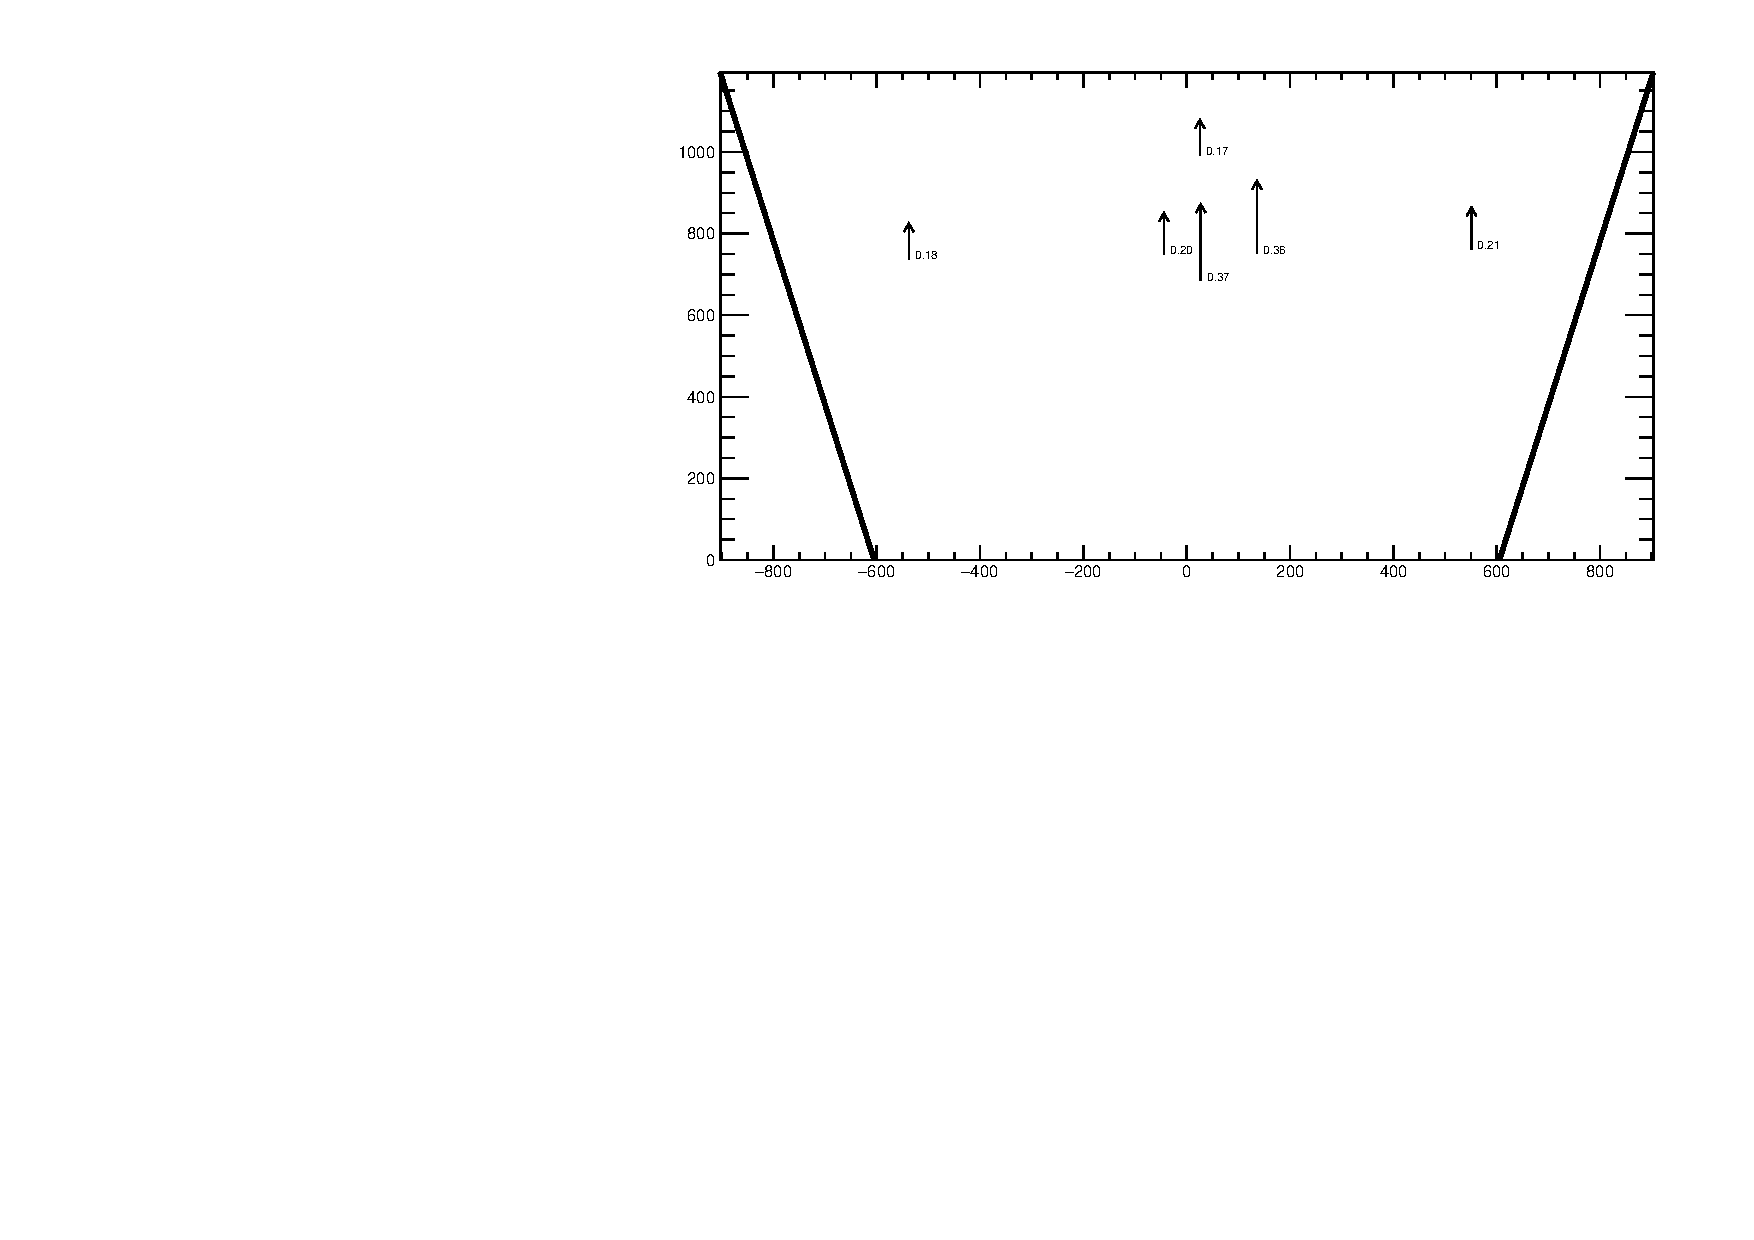
\includegraphics[width=\linewidth]{figures/QL2P11_xray_residuals_layer2_fixedlayers13.pdf}
  \caption{X-ray residuals on sTGC module QL2.P.11 layer 2 obtained using reference layers 1 and 3.}
  \label{fig:xray_res_th2_ql2p11}
\end{subfigure}%
\vspace*{\floatsep}
\begin{subfigure}{\textwidth}
  \centering
  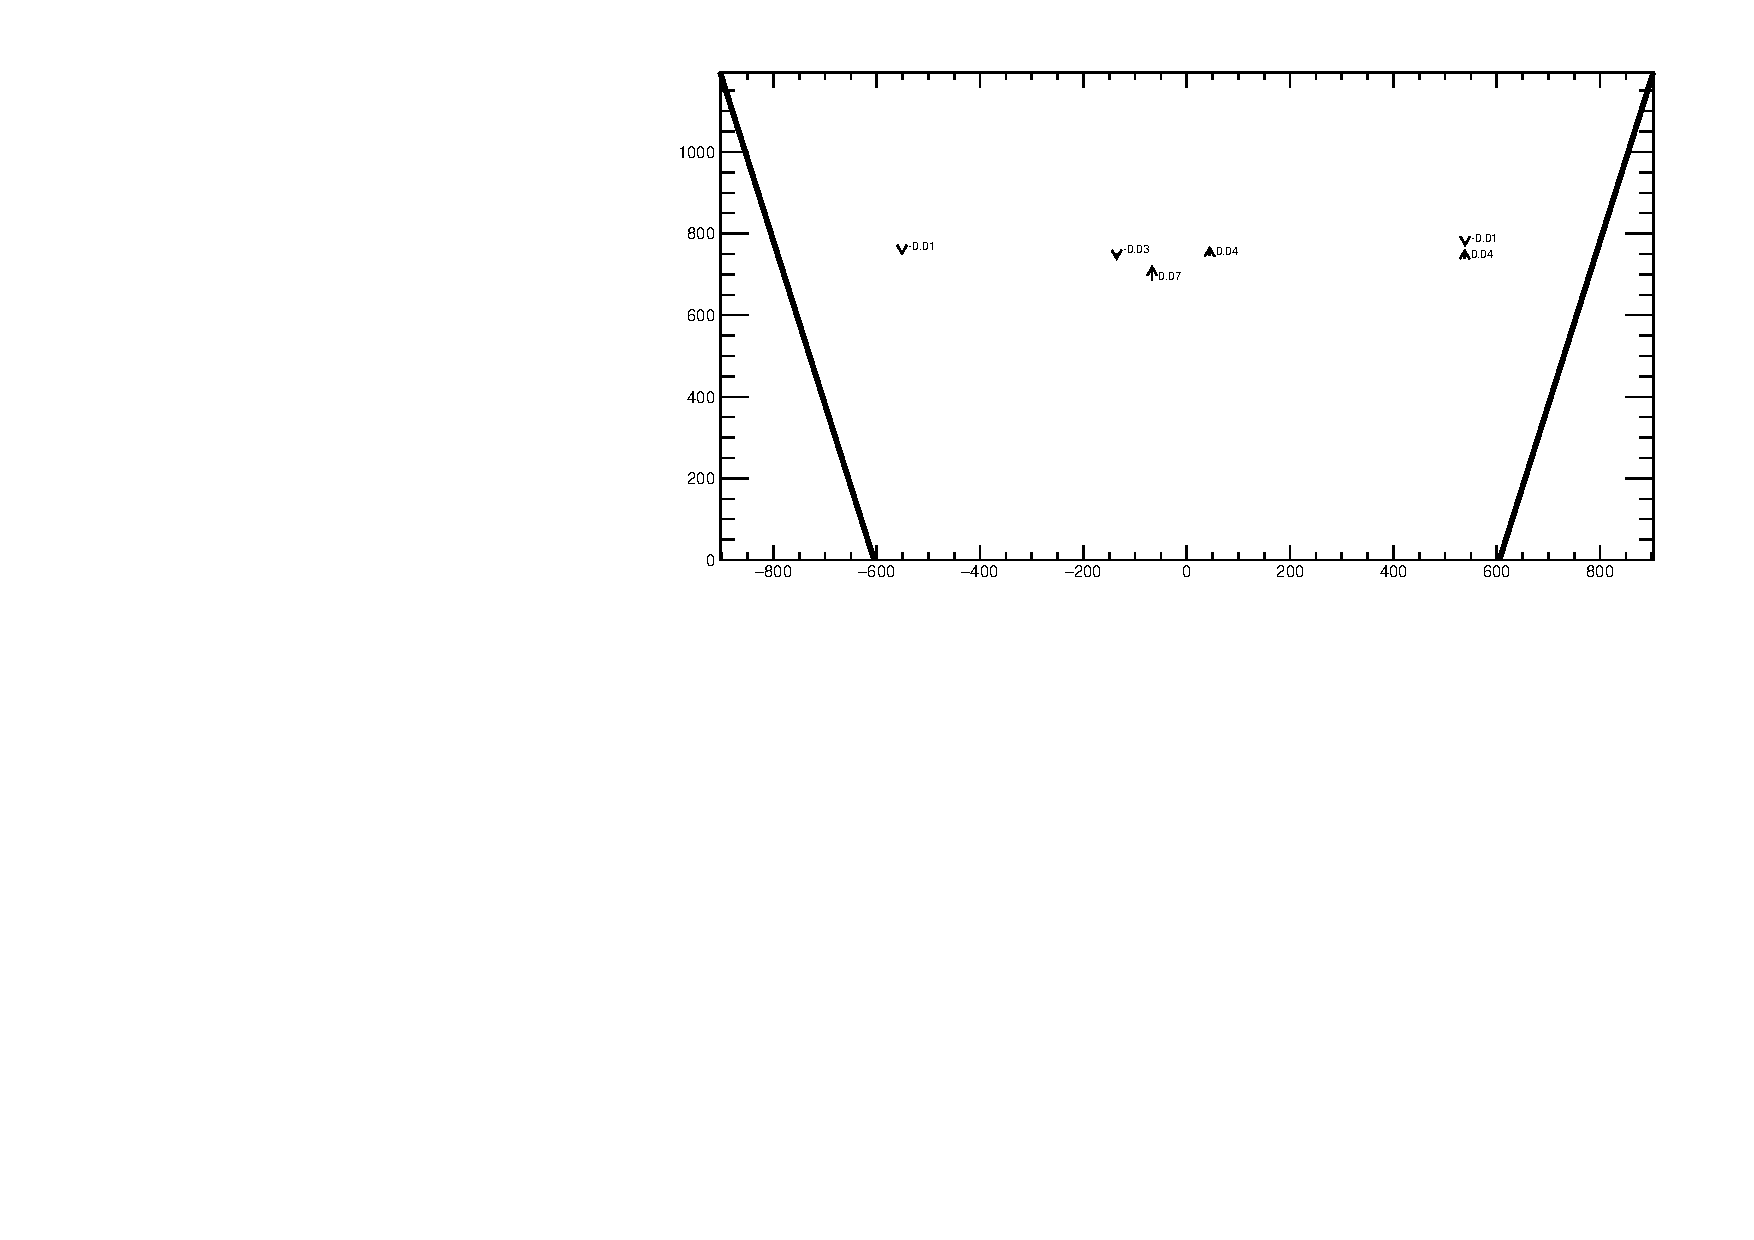
\includegraphics[width=\linewidth]{figures/QL2P08_xray_residuals_layer2_fixedlayers13.pdf}
  \caption{X-ray residuals on sTGC module QL2.P.8 layer 2 obtained using reference layers 1 and 3.}
  \label{fig:xray_res_th2_ql2p8}
\end{subfigure}
\caption{The x-ray residuals on sTGC layer 2 calculated with respect to the beam profile centers on sTGC layers 1 and 3 for sTGC modules QL2.P.11 (a) and QL2.P.8 (b). The arrows originate from the expected position of the beam profile center assuming a nominal geometry. The lengths of the arrows are 500 times the value of the x-ray residuals, scaled for visibility. The value of the x-ray residuals are annotated in millimeters and have an uncertainty of $\pm$\SI{0.15}{mm}.}
\label{fig:xray_res_th2}
\end{figure}
\newpage
\restoregeometry

For each x-ray survey position, the x-ray residual was calculated for all possible pairs of sTGC layers taken as reference and sTGC layers the track could be polated to (which required an x-ray beam profile on at least three layers), as was done for cosmic muon tracks. Figure~\ref{fig:xray_res_th2} shows the x-ray residual values on sTGC layer 2 with respect to reference layers 1 and 3 for sTGC quadruplet modules QL2.P.11 and QL2.P.8.  For module QL2.P.11, a negative relative local offset is measured at all x-ray survey points, indicating a global translation of sTGC layer 2 with respect to layers 1 and 3.

The uncertainty on the x-ray residualsis is obtained by propagating the uncertainty on the reconstructed x-ray beam profile centers (\SI{120}{\micro\meter}) through the polation. The uncertainty on the x-ray residuals ranges from \SI{0.15}{mm} to \SI{0.4}{mm} from the most to least geometrically-favourable tracking combination. There is no discernible pattern of misalignmnet revealed by the x-ray residuals on QL2.P.8 because they have absolute values smaller than the uncertainty on the x-ray residuals (\SI{150}{\micro\meter}). The x-ray residual uncertainties are significantly larger than the uncertainties on the means of cosmic track residual distributions. The relative local offsets calculated using cosmics data and x-ray data will be compared in the next chapter.
% ==================================================
% CHAPTER 7: Comparing cosmic muon and x-ray relative strip position offsets %
% ==================================================

\chapter{Comparing cosmic muon and x-ray relative strip position offsets}
\label{chap:comparison}
% Edit count: Lia - 1, Brigitte - 0

The goal of the work presented in this thesis is to validate the local strip position offsets measured with x-ray data with results obtained using cosmic ray data. The challenge was that the x-ray dataset provided absolute local offsets measured in the ATLAS coordinate system while the cosmics dataset provided relative local offsets measured with respect to a reference frame defined by two of four sTGC layers in a quadruplet~-- which could not be compared directly. To address the challenge, the x-ray local offsets were used to calculate relative local offsets. Relative local offsets on each sTGC layer obtained with x-ray and cosmics data calculated using the same two sTGC reference layers are compared for each area where x-ray data is available. The results of the comparison are presented here.

% The x-ray relative local offset is opposite sign to the x-ray residual reconstructed from an abstract track using the beam profile centers on each layer as the track hits. The cosmics relative local offset was inferred from the Gaussian mean of muon track residuals in a \SI{100}{mm} by \SI{100}{mm} area, referred to the as the mean cosmics residual.
% --------------------------------------------------
% \section{Evaluating}
% --------------------------------------------------


%---------------------------------------------------
\section{Results}
%---------------------------------------------------
\label{sec:results}

Relative local offsets have the same value but opposite sign to the mean cosmics and x-ray residuals. For the remainder of this chapter, the means of cosmic track residual distributions will be referred to as mean cosmics residuals. 

Mean cosmics and x-ray residuals on sTGC layer 2 calculated with reference layers 1 and 3 across the quadruplet surface are shown in figure~\ref{fig:res_compare_th2} for sTGC quadruplets QL2.P.11 and QL2.P.8. Figure~\ref{fig:res_compare_th2} is a superposition of figures~\ref{fig:res_mean_th2} and \ref{fig:xray_res_th2}.

\newpage
\thispagestyle{empty}
\newgeometry{top=0.5in,bottom=0.5in}
\begin{figure}
\centering
\begin{subfigure}{\textwidth}
  \centering
  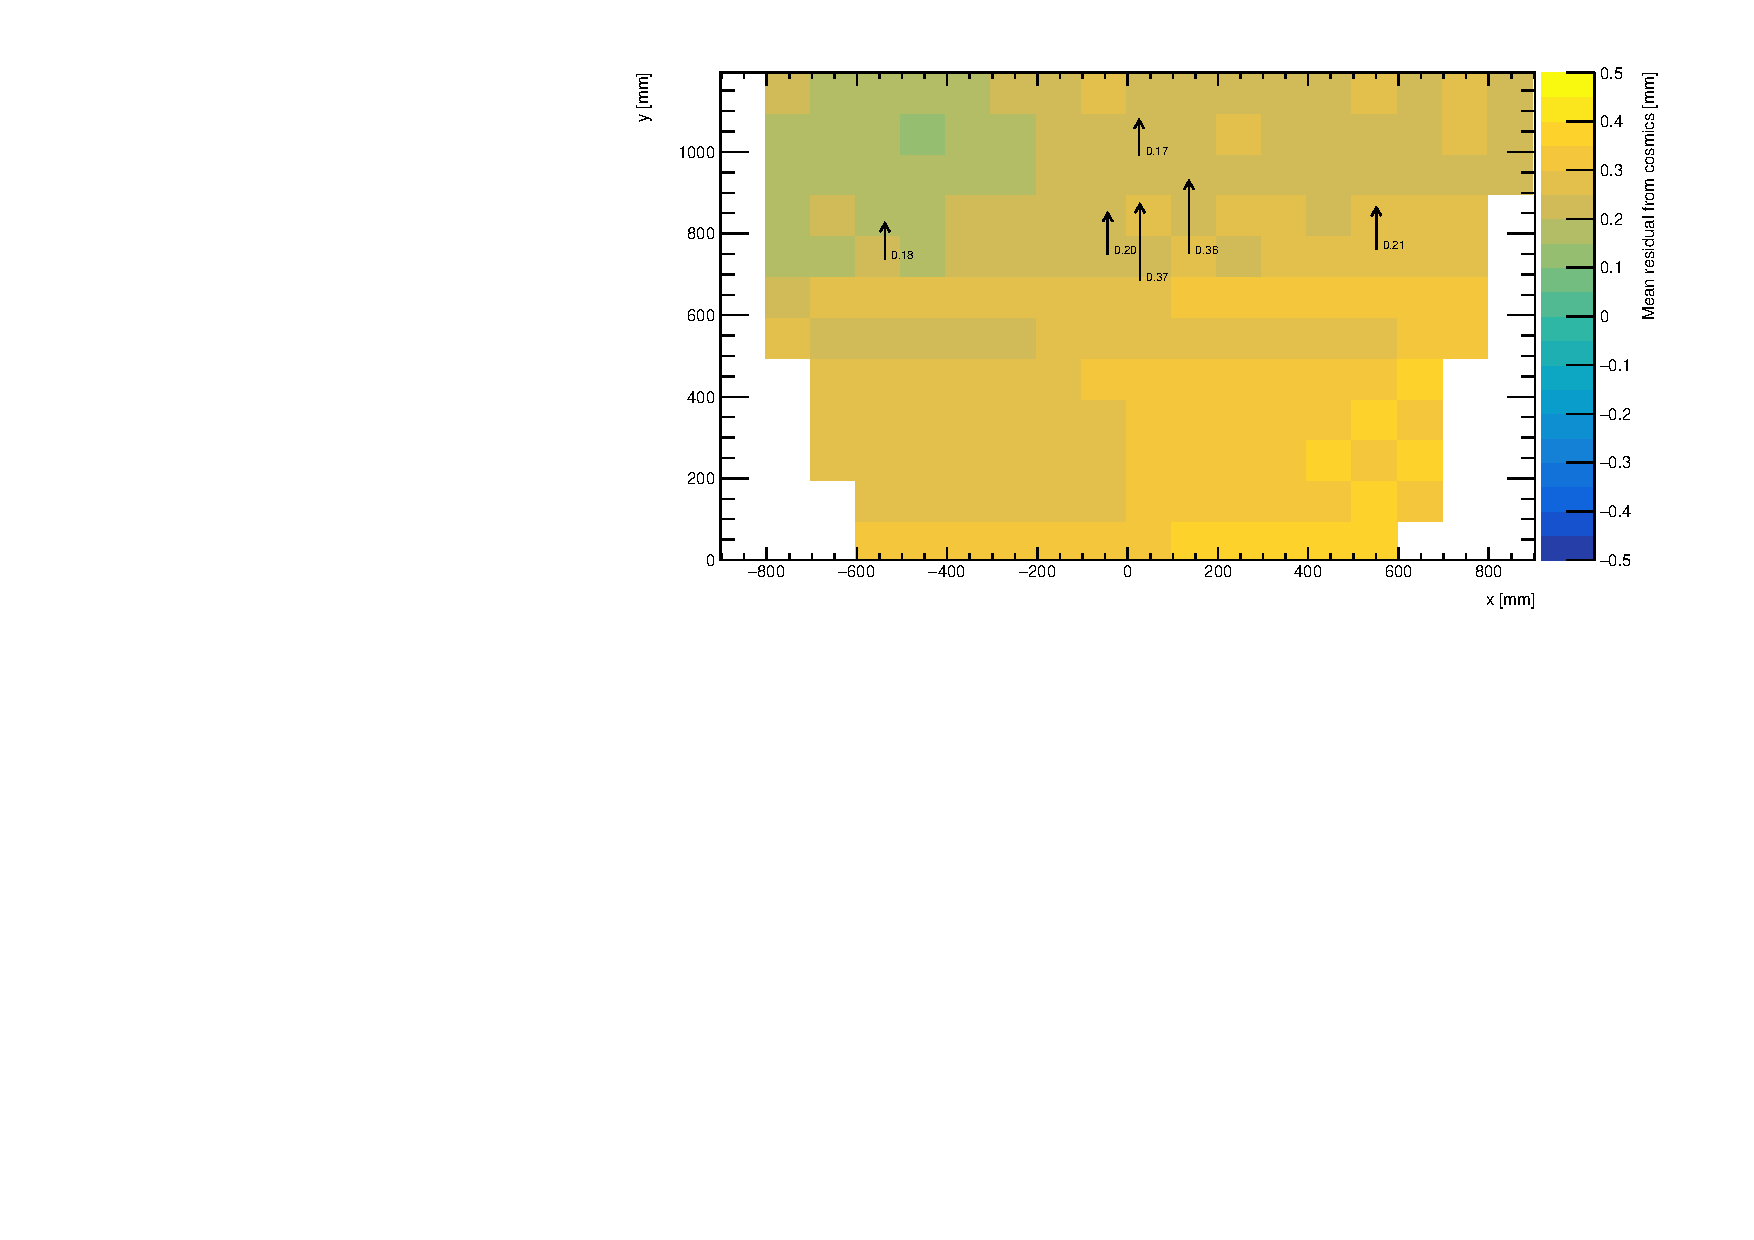
\includegraphics[width=\linewidth]{figures/QL2P11_compare_residuals_th2_layer2_fixedlayers13.pdf}
  \caption{Mean cosmics and x-ray residuals on sTGC layer 2 of quadruplet QL2.P.11 obtained using reference layers 1 and 3.}
  \label{fig:res_compare_th2_ql2p11}
\end{subfigure}%
\vspace*{\floatsep}
\begin{subfigure}{\textwidth}
  \centering
  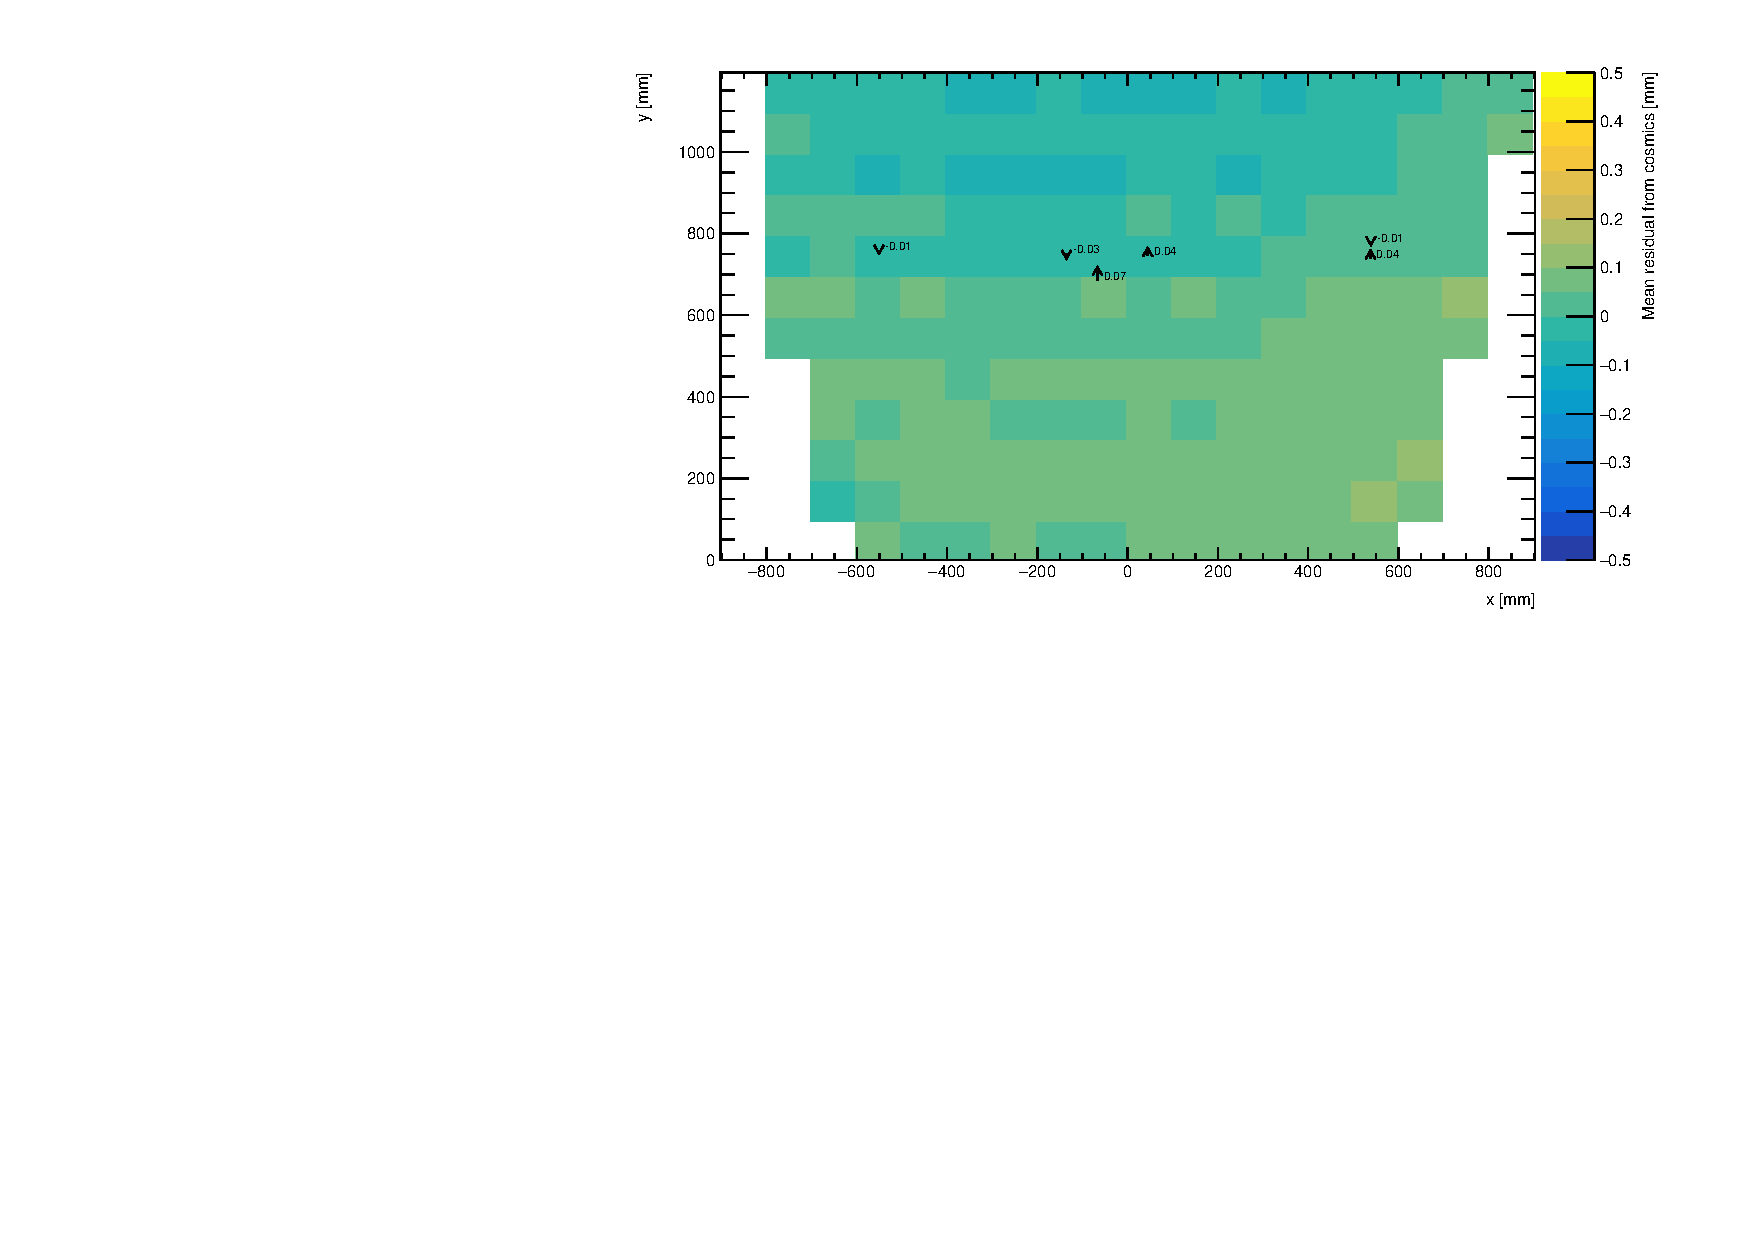
\includegraphics[width=\linewidth]{figures/QL2P08_compare_residuals_th2_layer2_fixedlayers13.pdf}
  \caption{Means cosmics and x-ray residuals on sTGC layer 2 of quadruplet QL2.P.8 obtained using reference layers 1 and 3.}
  \label{fig:res_compare_th2_ql2p8}
\end{subfigure}
\caption{The mean cosmics residuals are shown using colour. The x-ray residuals available at nominal gun positions are drawn as arrows and the value of the residual annotated in millimeters with uncertainty $\pm$\SI{0.15}{mm}. The length of the arrows is 500 times the value of the x-ray residual, scaled for visibility. These plots are a superposition of figures~\ref{fig:res_mean_th2} and \ref{fig:xray_res_th2}.}
\label{fig:res_compare_th2}
\end{figure}
\newpage
\restoregeometry

Figure~\ref{fig:res_compare_th2_ql2p11} shows that for QL2.P.11 the x-ray residuals are of the same sign and order as the mean cosmics residuals, as can be seen by comparing the annotated value of the x-ray residual to the mean cosmics residual represented in the nearest coloured bin. QL2.P.11's mean cosmics and x-ray residuals are correlated. 

For QL2.P.8, figure~\ref{fig:res_compare_th2_ql2p8} shows that the x-ray residuals are of the right order compared to the mean cosmics residuals; however, the value of the x-ray residuals are within their uncertainty so the correlation is not manifest. While the x-ray residuals do not reveal a pattern in the relative local offsets across the layer's surface, the mean cosmics residuals show a structure to the relative local offsets, revealed by how they vary smoothly over the surface of sTGC layer 2. 

The comparison of mean cosmics and x-ray residuals was done for several sTGC quadruplets for all possible tracking combinations. Scatter plots of the x-ray and mean cosmics residuals on QL2.P.11 and QL2.P.8 for all tracking combinations are shown in figures~\ref{fig:correlation} and \ref{fig:no_correlation} and reveal the degree of correlation between the datasets. In these correlation plots, each rectangle is centered on the value of a mean cosmics and x-ray residual pair calculated with a given tracking combination for every x-ray gun position where data is available. The height and width of the rectangles are the uncertainty in the mean cosmics and x-ray residuals respectively. Note that in the scatter plots, the regions of interest where cosmics tracks are included in the calculation of the mean of residuals are exactly centered on the nominal x-ray beam positions, unlike in figure~\ref{fig:res_compare_th2}.

\begin{figure}
    \centering
    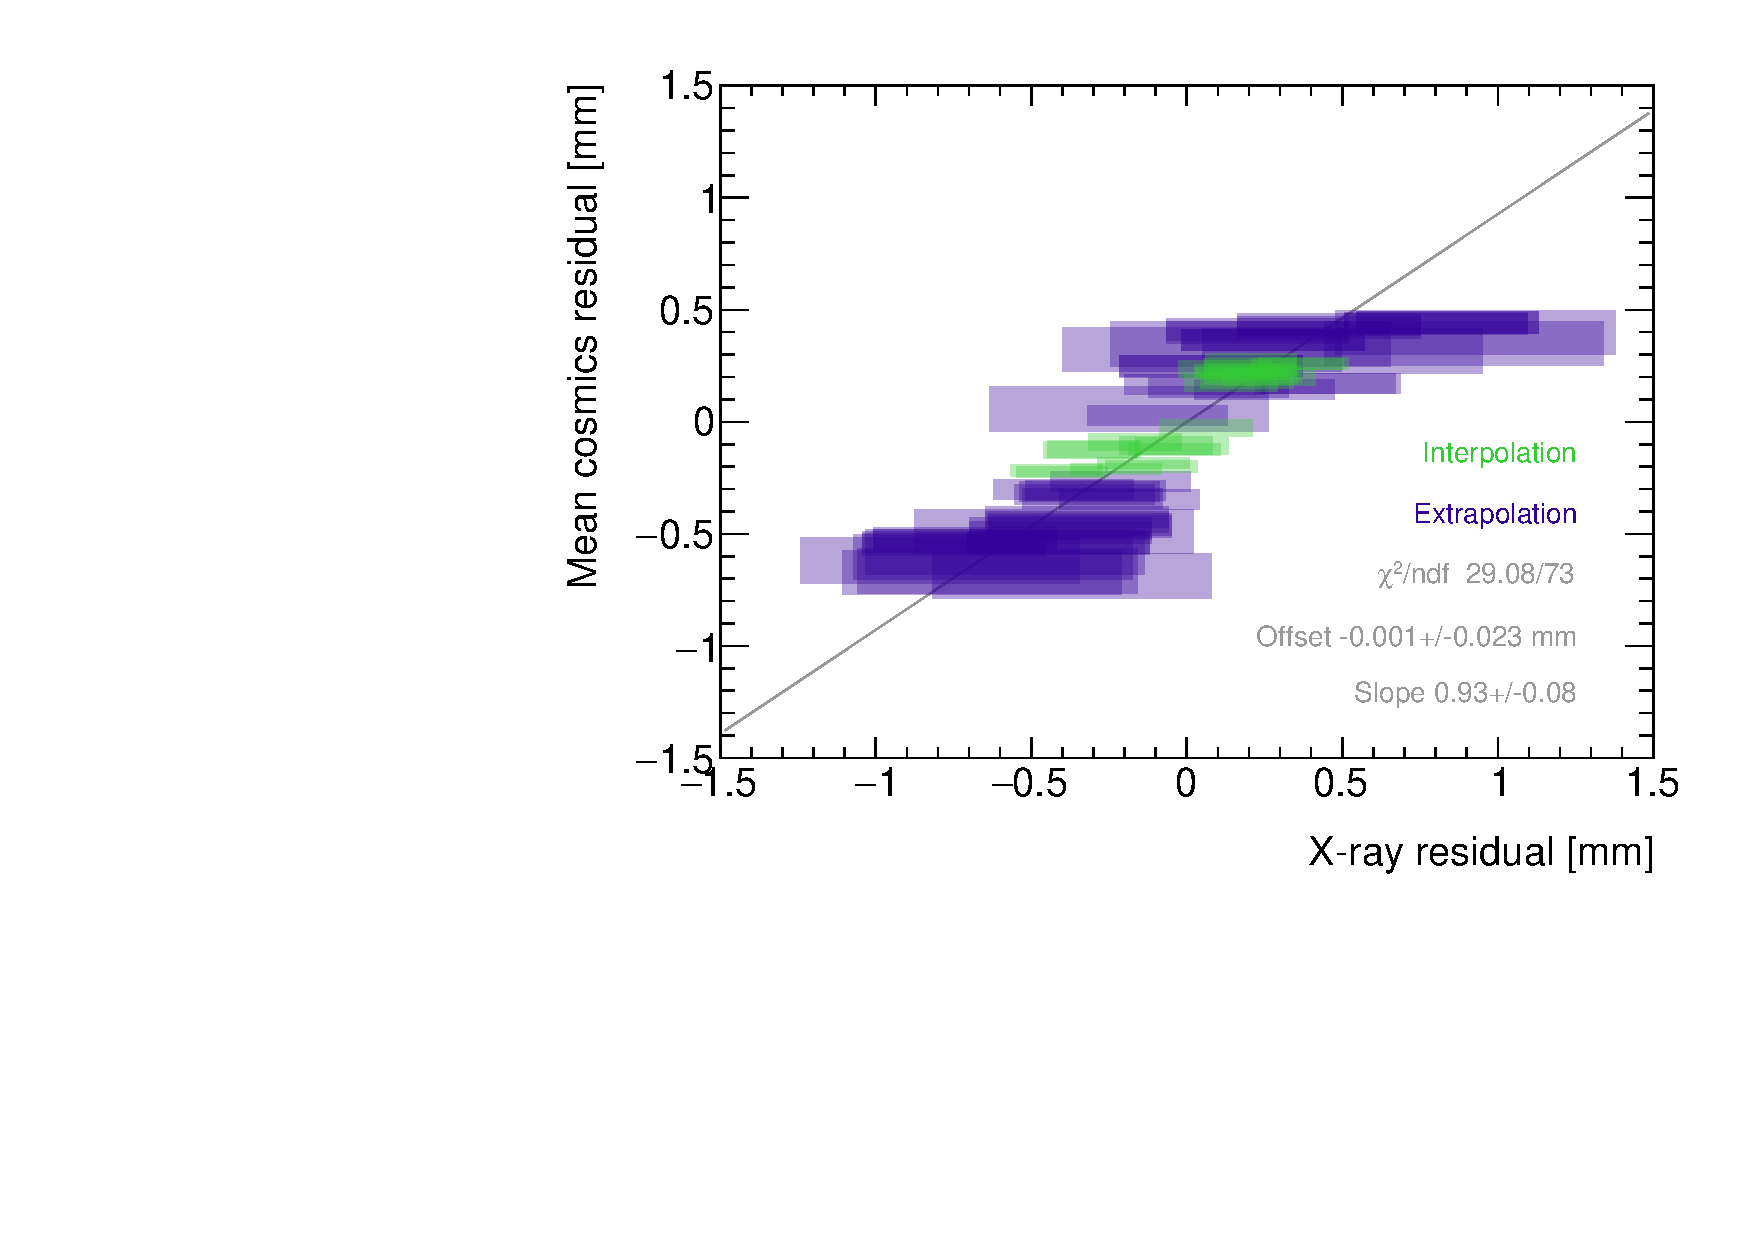
\includegraphics[width = \textwidth]{figures/figure_QL2P11_3100V_2021-08-05_QL2P11_local_cosmic_and_xray_data_correlation_plot.pdf}
    \caption{Correlation plot between x-ray and mean cosmics residuals for all tracking combinations for QL2.P.11. Each rectangle is centered on an x-ray and mean cosmics residual pair calculated at a given x-ray gun position and for a certain tracking combination. The width of the rectangles in $x$ and $y$ are the uncertainty in the x-ray and mean cosmics residual respectively. A printer-friendly version of this plot is available in appendix~\ref{appendix:print}.}
    \label{fig:correlation}
\end{figure}

The fitted slope and offset in figure~\ref{fig:correlation} show that the two QL2.P.11 datasets are correlated. The large uncertainty on the x-ray residuals set a limit on the sensitivity of the analysis, for if the absolute value of the x-ray residuals of a quadruplet were smaller than the x-ray residual uncertainties, no conclusion about the correlation could be drawn, as is the case for layer 2 of sTGC quadruplet QL2.P.8 (figure~\ref{fig:no_correlation}). This result is reflected in the small x-ray residuals shown in figure~\ref{fig:res_compare_th2_ql2p8} that do not reveal a pattern in the relative local offsets across the surface of sTGC layer 2. However, figure~\ref{fig:no_correlation} shows that the x-ray and mean cosmics residuals are clustered approximately around zero as is expected for a quadruplet with small relative misalignments between layers.

\begin{figure}
    \centering
    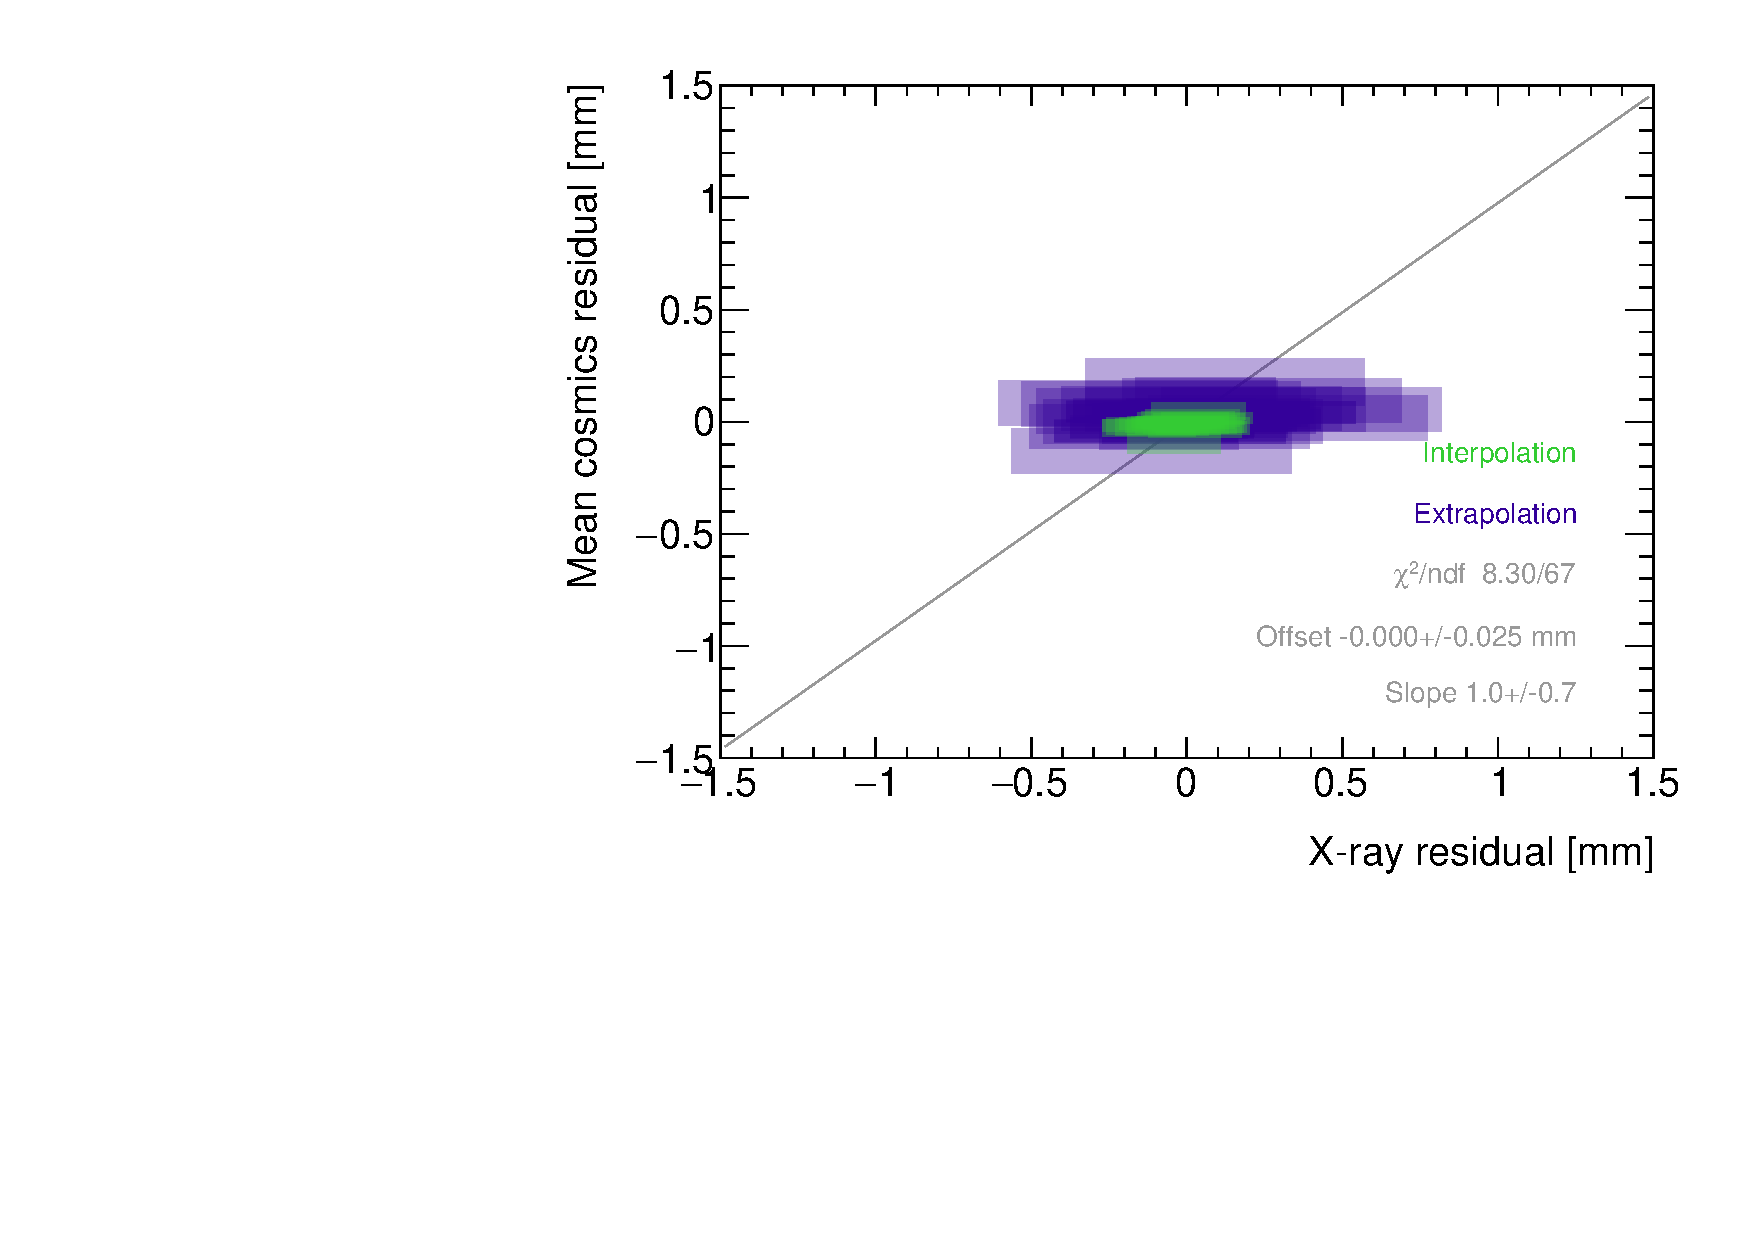
\includegraphics[width = \textwidth]{figures/figure_QL2P08_3100V_2021-08-16_QL2P08_local_cosmic_and_xray_data_correlation_plot.pdf}
    \caption{Correlation plot between x-ray and mean cosmics residuals for all tracking combinations for QL2.P.8. Each rectangle is centered on an x-ray and mean cosmics residual pair calculated at a given x-ray gun position and for a certain tracking combination. The width of the rectangles in $x$ and $y$ are the uncertainty in the x-ray and mean cosmics residuals respectively. A printer-friendly version of this plot is available in appendix~\ref{appendix:print}.}
    \label{fig:no_correlation}
\end{figure}

There are three patterns in the residuals on the scatter plot explained by geometry. First, for both datasets the uncertainty in the extrapolated track residuals were larger than the interpolated track residuals because of the extrapolation lever arm. For the x-ray residuals, the effect of the lever arm on the uncertainty was direct since the residual was calculated from a single straight line; for the mean cosmics residuals it is the widening of the residual distributions due to the extrapolation lever arm that increases the uncertainty in the fitted means of residuals. Second, residuals calculated through extrapolation tend to be larger because the extrapolation lever arm can produce more extreme values of the track position on the layer of interest. Third, the points in figure~\ref{fig:correlation} are geometrically correlated (e.g. they seem to be roughly mirrored around the origin). This is expected since the residuals calculated using a given set of three layers should be geometrically correlated by the local offsets on each layer (the $d_{local, i}$ on each layer as defined in equation~\ref{eqn:local_translation}). 

% --------------------------------------------------
\section{Discussion}
% --------------------------------------------------

Several sTGC quadruplets were tested for each quadruplet construction geometry built in Canada. Each quadruplet fell into one of the two categories: residuals large enough to see a correlation, or residuals too small to see a correlation. Since the x-ray and mean cosmics residuals can be used to calculate relative local offsets between the layer and the two reference layers, quadruplets with the largest relative misalignments had the largest range of residuals. The correlation plots are another easy visual way to identify quadruplets with large relative misalignments.

The most significant limit on measuring the degree of correlation between the x-ray and mean cosmics residuals is the uncertainty on the x-ray residuals, which stemmed from the systematic uncertainty of \SI{120}{\micro\meter} in the x-ray beam profile centers used to construct the straight lines. For example, in figure~\ref{fig:no_correlation}, if the x-ray residuals could be known to within better precision, perhaps they would be correlated with the mean cosmics residuals. The x-ray method was limited primarily by the systematic uncertainties in the relative alignment of the alignment platforms and the gun, especially the gun angle.

The analysis of a fraction of the sTGC quadruplets was limited by the availability of data. Sometimes, less than three sTGC layers in a quadruplet were surveyed for a given x-ray gun position so no residuals could be calculated. Too few x-ray residuals prevented the analysis from detecting a significant correlation with cosmics data, should it even be measurable. Often, the analysis of sTGC quadruplets of smaller sizes (placed innermost on the wheel) is limited because they have fewer alignment platforms, and hence gun positions, on their surfaces as a result of their size. The analysis is also limited to a fraction of all sTGC quadruplets built. The wedges constructed the earliest (typically small wedges) were surveyed when the x-ray method was still being designed, so a limited number of x-ray residuals can be calculated and the beam profiles were of lower quality. 
% Limiting to Canadian modules
%In addition, not all cosmic muon test sites had enough front end electronics to collect data on three layers simultaneously, which is the minimum required to be able to calculate residuals.

Nonetheless, the comparison of x-ray and mean cosmics residuals was really to confirm the x-ray method's ability to measure local offsets with an independent dataset. The x-ray local offsets allow the calculation of relative local offsets that have been correlated to the cosmics relative local offsets. Therefore, the analysis of quadruplets with relative local offsets large enough to detect a correlation validates the x-ray method's ability to measure local offsets. 

The potential of using relative local offsets calculated from cosmics data to study relative alignment between sTGC layers stands on its own. For example, although the x-ray residuals in QL2.P.8 in figure~\ref{fig:res_compare_th2_ql2p8} do not reveal a pattern, the variation in the mean cosmics residuals do. Identifying the pattern is possible because mean cosmics residuals can be calculated across the entire sTGC layer's area and are sensitive to smaller relative local offsets since their uncertainty is significantly smaller. 

% The advantage of the x-ray dataset over the cosmics dataset is that absolute local offsets are measurable thanks to the reference frame provided by the alignment platforms. This is required to measure the position of strips in the ATLAS coordinate system and to satisfy the NSWs' precision tracking goals. The x-ray local offsets are being used to build an alignment model of strips in each quadruplet. It is compelling to imagine using the cosmics relative local offsets to improve the model considering their precision and ability to capture effects across the entire area of the quadruplet.

% --------------------------------------------------
\section{Next steps}
% --------------------------------------------------

The results presented in this thesis pave the way to the further application of the rich cosmic muon data set to alignment work. First, a systematic study of cosmic ray and x-ray relative local strip position offsets should be performed for all quadruplets built for the NSWs. The correlation plots such as those presented in figure~\ref{fig:correlation} and~\ref{fig:no_correlation} can reveal unexpected results which could indicate an issue with either cosmic ray or x-ray data collection to be investigated further. Then, the overall correlation between x-ray and cosmic datasets should be quantified for all quadruplets instead of being quantified for each quadruplet individually.
 
For now, the correlation of the individual quadruplets tested supports the use of the x-ray data to build an alignment model. The plan is that the alignment parameters will be provided to the ATLAS experiment's offline software to estimate the position of each strip and so improve precision muon tracks reconstruction using the sTGCs. Work on the alignment model is ongoing~\cite{lefebvre_precision_2020}. Currently, the algorithm compares the offsets of a local group of strips at each x-ray gun position as measured by the x-ray and CMM methods in a fit to extract a global slope ($m$) and offset ($b$) per layer, $i$, where the $\chi^2$ is given by equation~\ref{eqn:chi2}.

\begin{equation}
    \chi^2 = \frac{\left[dy_{cmm, corr} - dy_{xray}\right]^2}{\delta dy_{xray}^2 + \delta dy_{cmm, corr}^2}\:,
    \label{eqn:chi2}  
\end{equation}
\begin{equation}
    dy_{cmm, corr} = y_{cmm} + b_i + m_{i}x - y_{nom}
    \label{eqn:dy_cmm_corr}
\end{equation}

Here, $dy$ is a local strip position offset as calculated from the x-ray and corrected CMM data and $\delta dy$ refers to their respective uncertainties. The large uncertainty on the x-ray local offsets (\SI{120}{\micro\meter}) and the sparseness of the measurements means that including input from other characterization datasets could reduce the uncertainty on the alignment model parameters. 

Work on adding the relative local strip position offsets measured using cosmic ray data to the alignment model has begun. They provide alignment information between the x-ray measurement points and can be calculated with a precision relevant to alignment studies. Therefore, they provide additional and complementary information that could further constrain the global rotation and translation parameter of the simple misalignment model currently being used. It is compelling to imagine improving the accuracy of the alignment model given that the accuracy to which the positions of the strips are known in ATLAS will affect the quality of the reconstructed muon tracks used to study high energy physics processes.

%The CMM measurements were taken before the cathode boards were assembled into quadruplets, so alignment parameters for the given layer were extracted from the $\chi^2$ fit by stepping the corrected CMM $y$-position towards the x-ray $y$-position by adjusting the layer's slope and offset parameters.
%The uncertainty in the mean cosmics residuals was smaller than the desired position resolution of the sTGCs, so they provide relevant information about strip positions. Moreover, they can be calculated over the entire area of the quadruplet instead of at specific positions. It would be great to use the cosmics residuals as input to calculate and reduce the uncertainty on the alignment parameters. Since mean cosmics residuals can only provide relative alignment information, one idea would be to use them to constrain the fit of the alignment parameters. In this case, the alignment parameters would need to be fitted on all layers at once, and the shifting y-positions on each layer forced to create an abstracted track residual equal to the local mean cosmics residual (within uncertainty) for each x-ray point. Or, instead of constraining the fit, it could be penalized if the resulting parameters do not result in abstracted track residuals equal to the mean cosmics residuals within uncertainty. Some work on using the three datasets at once in a fit has been started.
% ==================================================
% CHAPTER 8: Summary and Outlook %
% ==================================================

\chapter{Summary and outlook}
\label{chap:outlook_and_summary}
% Edit count: Lia - 1, Brigitte - 0

The LHC~\cite{evans_lhc_2008} will be at the energy frontier of particle physics for at least the next decade, making it a unique tool with which to study particle physics. With the HL-LHC~\cite{hl_lhc_tdr}, high statistics on rare particle physics processes will enable more precise measurements of parameters of the Standard Model and increase the sensitivity to signatures of physics beyond the Standard Model~\cite{dainese_physics_2018}. To capitalize on the increased luminosity, the muon small wheels of the ATLAS experiment must be replaced to keep the current triggering and tracking performance~\cite{nsw_tdr}. 

sTGCs are gas ionization chambers optimized for a high rate environment~\cite{nsw_tdr}. Using the pad electrodes to define a region of interest makes it possible to get track segments of $\sim$\SI{1}{mrad} angular resolution quickly, which will be used as input to check if a collision originated from the interaction point and whether it should be triggered on~\cite{nsw_tdr, perez-codina_small-strip_2016}. Thanks to the careful design of the sTGCs, particularly the small pitch of the strip readout electrodes, the sTGCs are able to provide better than \SI{100}{\micro\meter} position resolution per detector plane to fulfill precision offline tracking requirements~\cite{abusleme_performance_2016}. 

Ultimately, the positions of the sTGC strip electrodes need to be known in ATLAS to within $\sim$\SI{100}{\micro\meter} so that they can deliver the required position resolution~\cite{nsw_tdr}. The strategy is to build an alignment model to estimate the position of each strip~\cite{lefebvre_precision_2020}. Input to the alignment model comes from the datasets used to characterize the quadruplets. The x-ray data~\cite{lefebvre_precision_2020} is the only characterization dataset that directly links the position of the strips to the ATLAS coordinate system. The alignment model could be built on x-ray data alone, but the sparseness of and large uncertainty on the local offsets mean that the alignment model could benefit from more input. The x-ray method is also a new technique that should be independently validated.

Relative local offsets measured with the cosmics and x-ray datasets were compared and the observed correlation confirmed the local offsets measured with the x-ray gun. Moreover, the cosmics relative local offsets are useful on their own. The 2D visualizations of relative local offsets make it possible to quickly identify areas of misaligned strips and make hypotheses as to the physical origin of those misalignments. Also, the cosmics residual means were shown to be robust and have uncertainties under \SI{100}{\micro\meter} for all two-fixed-layer reference frames, which is small in this context. Therefore, the cosmics relative local offsets complement the x-ray data by providing a complete, robust picture of the relative strip position offsets between layers. The next goal will be to use the cosmics relative local offsets to improve the alignment model and better position the sTGC strips in ATLAS.

Muons are important signatures of electroweak and Higgs sector events that physicists anticipate studying with a high-statistics dataset~\cite{dainese_physics_2018, nsw_tdr}. An effective alignment model of sTGC strip positions will ensure that the NSWs can be used to accomplish the ATLAS collaboration's physics goals during the High Luminosity era of the LHC.

% --------------------------------------------------
% \section{Importance in context}
% --------------------------------------------------
% \label{sec:importance}

%Ultimately, the positions of the sTGC strip electrodes need to be known in ATLAS to within $\sim$\SI{100}{\micro\meter} so that they can provide the required position resolution for the High-Luminosity LHC. The x-ray measurements will account for offsets of strips from their nominal position to achieve this goal. The cosmics dataset was used to confirm the local offsets measured with the x-ray gun, and could be used to improve the alignment model that will position each strip.

%Achieving the required position resolution on each layer of the NSWs in the particle track bending plane achieves the design momentum resolution for muons ejected towards the end-caps of ATLAS. Muons are important signatures of electroweak and Higgs sector events of interest for the ATLAS Collaboration's future physics goals~\cite{nsw_tdr}. Being the second of two tracking technologies on the NSWs, an effective alignment model of sTGC quadruplets is a necessary part of making the NSWs redundant for 10 or more years of recording collisions in the High Luminosity era of the LHC. 

%----------------------------------------------------------------------
% END MATERIAL
% Bibliography, Appendices, Index, etc.
%----------------------------------------------------------------------

% Bibliography

% The following statement selects the style to use for references.  
% It controls the sort order of the entries in the bibliography and also the formatting for the in-text labels.
% Tony used unsrt in his PhD thesis
\bibliographystyle{unsrt}
% This specifies the location of the file containing the bibliographic information.  
% It assumes you're using BibTeX to manage your references (if not, why not?).
% \cleardoublepage % This is needed if the "book" document class is used, to place the anchor in the correct page, because the bibliography will start on its own page.
% Use \clearpage instead if the document class uss the "oneside" argument
\phantomsection  % With hyperref package, enables hyperlinking from the table of contents to bibliography             
% The following statement causes the title "References" to be used for the bibliography section:
\renewcommand*{\bibname}{References}

% Add the References to the Table of Contents
\addcontentsline{toc}{chapter}{\textbf{References}}

\bibliography{thesis}
% Tip: You can create multiple .bib files to organize your references. 
% Just list them all in the \bibliogaphy command, separated by commas (no spaces).

% The following statement causes the specified references to be added to the bibliography even if they were not cited in the text. 
% The asterisk is a wildcard that causes all entries in the bibliographic database to be included (optional).
\nocite{*}
%----------------------------------------------------------------------

% Appendices

% The \appendix statement indicates the beginning of the appendices.
\appendix
% Add an un-numbered title page before the appendices and a line in the Table of Contents
\chapter*{APPENDICES}
\addcontentsline{toc}{chapter}{APPENDICES}
% Appendices are just more chapters, with different labeling (letters instead of numbers).
% ==================================================
% Appendix: Uncertainty in cluster positions %
% ==================================================

%TODO : Organize figure positioning once you're done writing. 

\chapter[Cluster position uncertainty]{Uncertainty in cluster positions}
\label{appendix:clustering}

% Cluster def
% Cluster x from wires, cluster y from strips
% Cluster x uncertainty
% Cluster y statistical uncertainty
% Cluster y systematic uncertainty depending on choice of fitting algorithm

%TODO : What causes variation in cluster size? Why do we see changes in relative cluster size populations between 2900 V and 3100 V data? Benoit's thesis, page 36, references. Need this to correct red sentence.
A cluster is a series of contiguous strip channels on a layer with non-zero amplitude, all part of the same trigger and having the same event number~\cite{lefebvre_thesis}. \textcolor{red}{Clusters result from a muon ionizing gas in the gap, and the number of strips in the corresponding cluster depends on the angle of the track and the gain (operating voltage)}. The peak-detector-output (PDO) of the signal on each strip of a cluster is fit with a Gaussian. The y-position of a particle as it passed through the layer is mean of the cluster, referred to here as the hit position.

The uncertainty assigned to the hit position affects the uncertainty in the calculated residuals, and so informs the appropriate bin width for the residual distributions. There is a statistical uncertainty in the hit position from the estimation of the Gaussian mean, but also a systematic uncertainty that depends on the fit algorithm used. 

The clusters were fit with Guo's method~\cite{guo_simple_2011} and Minuit2 for ROOT~\cite{hatlo_developments_2005}. The difference in cluster means between the two algorithms is shown in figure~\ref{fig:mu_reclustering_minus_mu_cosmics}.

%TODO : Make this figure pretty with a nicer text box?
\begin{figure}
    \centering
    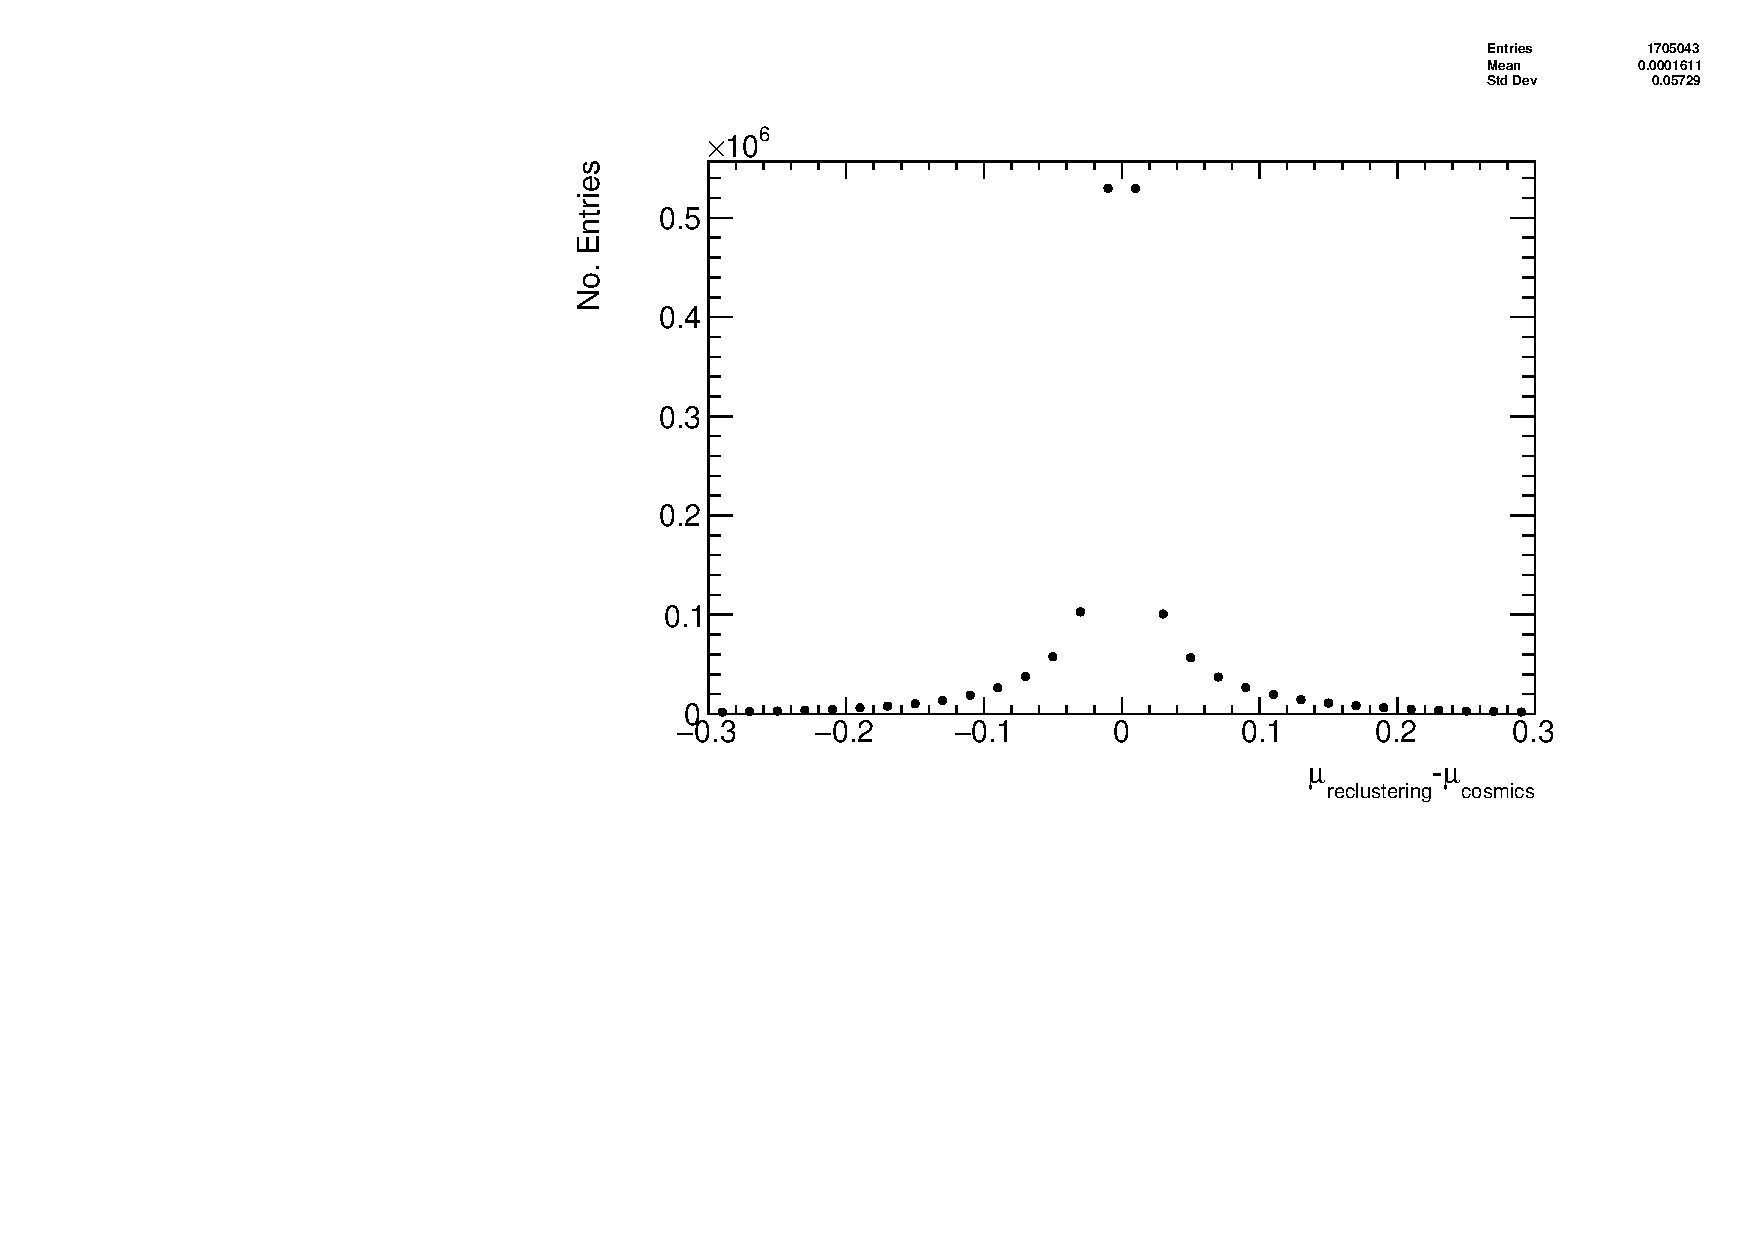
\includegraphics[width = 0.7\textwidth]{figures/figure_QL2P08_3100V_2021-05-21_reclustering_plots_mu_reclustering_minus_mu_cosmics.pdf}
    \caption{The difference between cluster means calculated with Guo's method~\cite{guo_simple_2011} in \package{tgc\_analysis/CosmicsAnalysis} and Minuit2 for ROOT~\cite{hatlo_developments_2005} in \package{strip\_position\_analysis/ReClustering} for data collected with QL2.P.8 at 3.1~kV.}
    \label{fig:mu_reclustering_minus_mu_cosmics}
\end{figure}

The RMS of the distribution in figure~\ref{fig:mu_reclustering_minus_mu_cosmics} is \SI{57}{\micro\meter}, which is much larger than the statistical uncertainty in the mean for the Minuit2 algorithm, which peaks around \SI{7}{\micro\meter}. An RMS of \SI{57}{\micro\meter} is common for data taken with most quadruplets at 3.1~kV. Therefore, the uncertainty in the y-hit positions is assigned \SI{57}{\micro\meter}.

%TODO : How does this inform the residual distribution bin size?

The x position of the cluster is taken to be the center of the wire group with the maximum detected signal, since wire groups are wide enough that usually only one wire picks up the ionization avalanche. 

%TODO : How does this inform the area of the bins we take residual means in?

%TODO : How does reclustering affect residual means?

% ==================================================
% Appendix: Analysis Statistics %
% ==================================================

\chapter[Analysis statistics]{Study of cosmics for alignment analysis statistical uncertainty}
\label{appendix:statistics}
% Edit count: 0

% Plan:
% Quantity of interest is the Gaussian mean of the residual distribution in a region of interest.
% Typically, have 1 million triggers; for QS3.P.18 got 3.5 million triggers.
% See the drop off in peak residual mean error with more triggers (FIGURE).
% We are not statistically limited. Compare residual fits for L1 F34 between 1 million triggers and 3.5 million triggers: means don't change significantly.

Typically, one million triggers (cosmic muon events, noise, photons and $\delta$-rays) were collected for each Canadian quadruplet at McGill University, resulting in roughly half the number of viable tracks after cuts. For QS3.P.18, 3.5 million triggers were collected. To gauge the sensitivity of the analysis to the available statistics, partitions of this data with each with a different number of triggers were analyzed separately. Ultimately, the quantity of interest was the Gaussian mean of the residual distribution in regions of interest, so the peak in the distribution of the statistical uncertainty in the residual means for each area of interest for a specific tracking combination was used to gauge the quality of the analysis. How the peak in the residual mean uncertainty distribution changes with the number of triggers is shown in figure for tracks on layer 1 built from layers 3 and 4 \ref{fig:res_mean_uncert_vs_triggers}. 

\begin{figure}
    \centering
    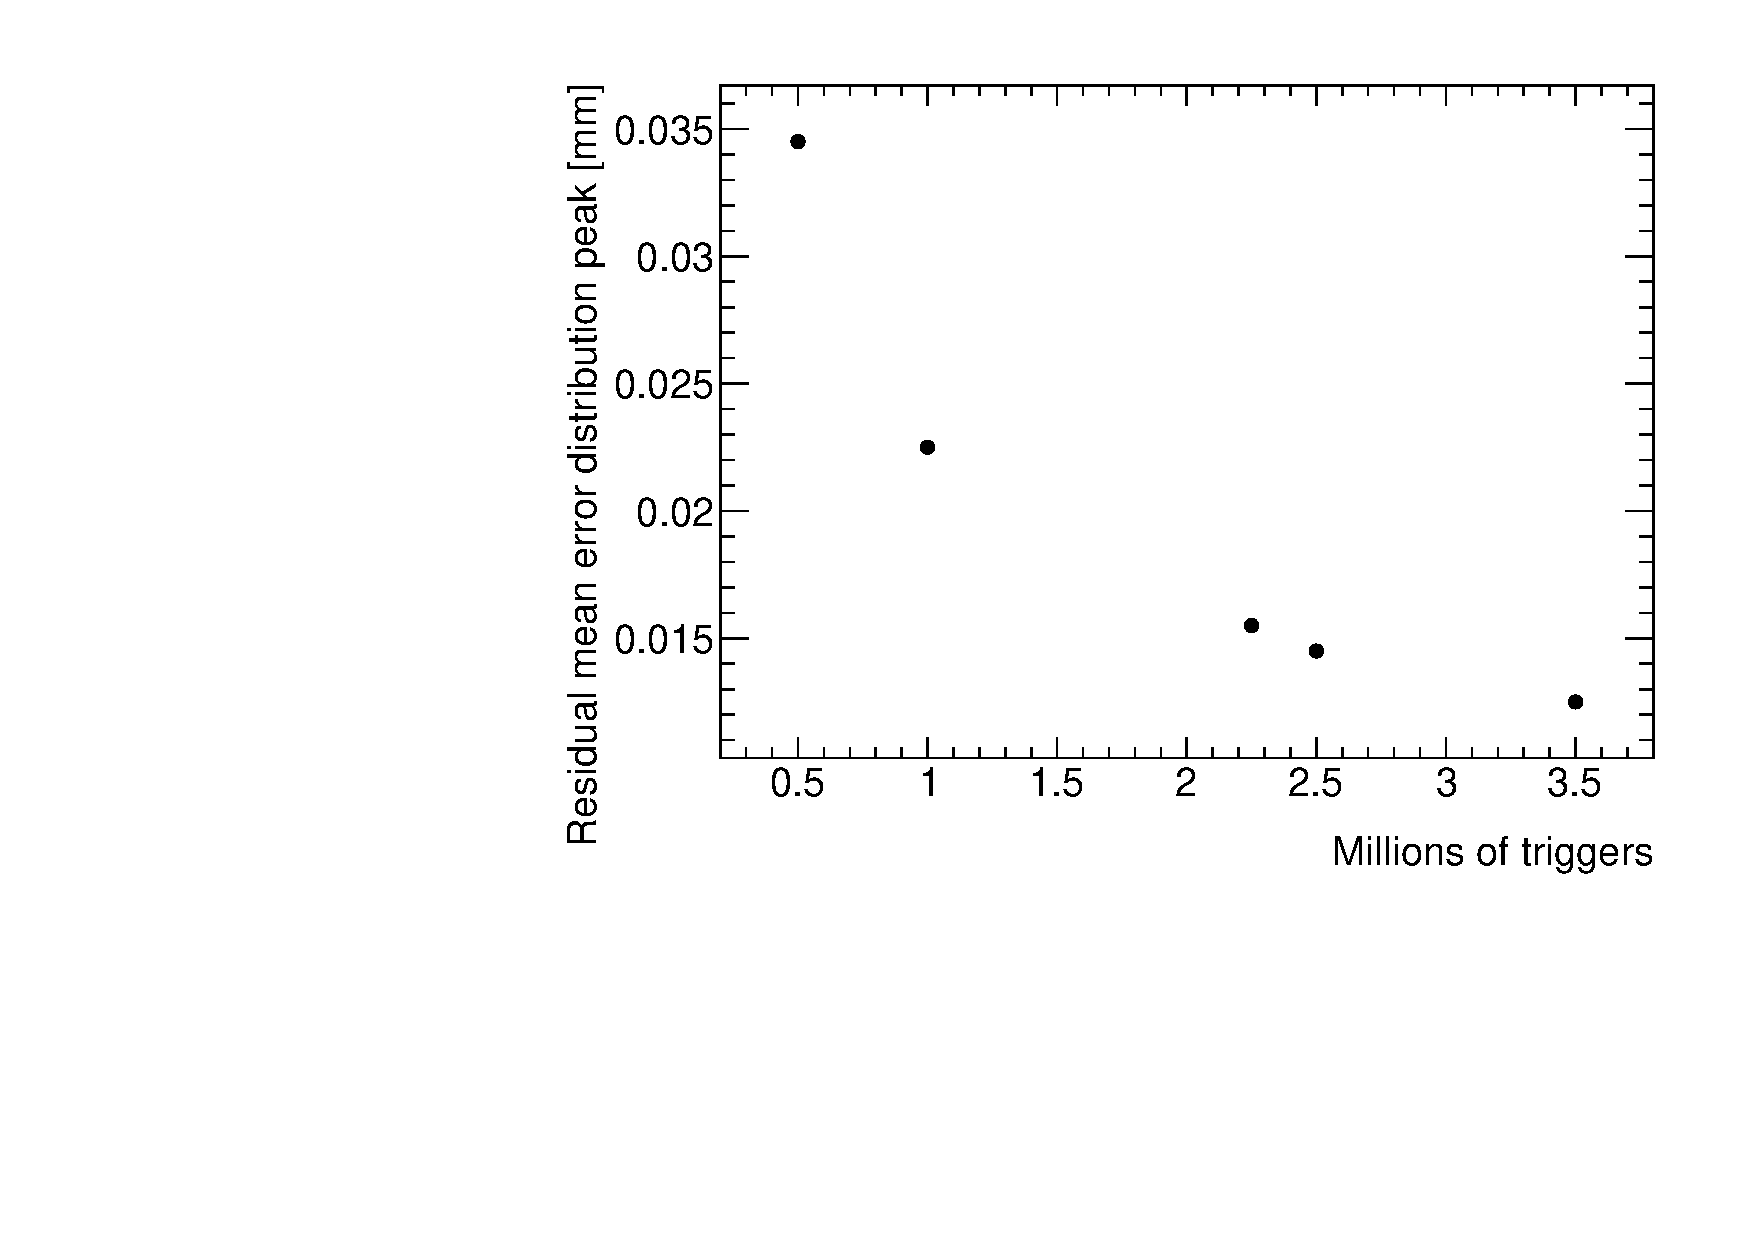
\includegraphics[width = \textwidth]{figures/figure_QS3P18_2900V_peakOfMeanErrorsDistVsTriggers_layer1_fixedlayers34.pdf}
    \caption{How the peak of the distributions of uncertainties in the residual means in regions ofinterest for tracks on layer 1 built from layers 3 and 4 changed with the number of triggers used in the analysis. The distribution falls off as $~\frac{1}{\sqrt{N}}$ as expected.}
    \label{fig:res_mean_uncert_vs_triggers}
\end{figure}

The uncertainty is already around \SI{20}{\micro\meter} at 1 million triggers, suitable for distinguishing differences in offsets of order \SI{50}{\micro\meter} as required. Although increased statistics could decrease the statistical uncertainty, it is not required for the goals of this analysis. Moreoever, the systematic uncertainty on the mean cosmics residuals is around \SI{50}{\micro\meter} so the statistical uncertainty of \SI{20}{\micro\meter} is nearly negligible.

%TODO : Include compare residual fit means for L1 F34 1 million vs 3.5 million triggers?? Do once you know how to make figures.

% ==================================================
% Appendix: Analysis Systematics %
% ==================================================

%TODO : Make mean diff plots not full page portrait. Half page would suffice. 
%TODO : Currently, section A.2 figure goes in A.3 section. Organize this once you're done writing. 
%TODO : Do I need to specify each quad? The voltage? 

\chapter[Analysis systematics]{Study of cosmics for alignment analysis systematic uncertainties}
\label{appendix:systematics}

% Sections:
% Doub gaus vs gaus -- check!
% Area bin size -- check!
% Residual distribution bin size?
%TODO 2900V vs 3100V? I think just saying strip efficiency is higher for 3100V is sufficient, although the sigmas are also smaller. But L4 F12 residual mean difference RMS is 74 um ==> Add 2900V 3100V section
% DNL
% ReClustering fit function? I think just saying I used an accepted standard is ok.

% --------------------------------------------------
\section{Residual distribution fit function}
% --------------------------------------------------
\label{appendix:systematics_res_fit_fcn}
% Edit count: 1

The distribution of residuals should be modelled by a double gaussian fit\cite{lefebvre_thesis}:

\begin{equation}
\label{eqn:doub_gaus}
G(r) = A_{s}exp\left[ \frac{-(r-\mu)^{2}}{2\sigma_s^{2}} \right] + A_{b}exp\left[ \frac{-(r-\mu)^{2}}{2\sigma_b^{2}} \right]
\end{equation}

where $r$ is the residual, $A$ is the gaussian amplitude, $\mu$ is the gaussian mean, $\sigma$ is the gaussian sigma, and the subscripts $s$ and $b$ stand for signal and background respectively. One gaussian captures the real (signal) tracks and the other captures the tracks built from noise (background). The gaussian with the smaller width is identified as the signal. 

A single gaussian fit failed less often than a double gaussian fit. The gaussian fits were performed by initially estimating the amplitude to be 100 tracks, the gaussian mean to be the histogram mean, and gaussian $\sigma$ to be the RMS. The fit range was restricted to $\pm$1 RMS from the histogram mean. The modification helped the gaussian fit capture the signal peak. An example residual distribution is shown in figure \ref{fig:double_gaussian_example_fit}. 

%TODO Why is this figure blurry?
%TODO this doesn't need to be a full page figure.

\begin{figure}
    \centering
    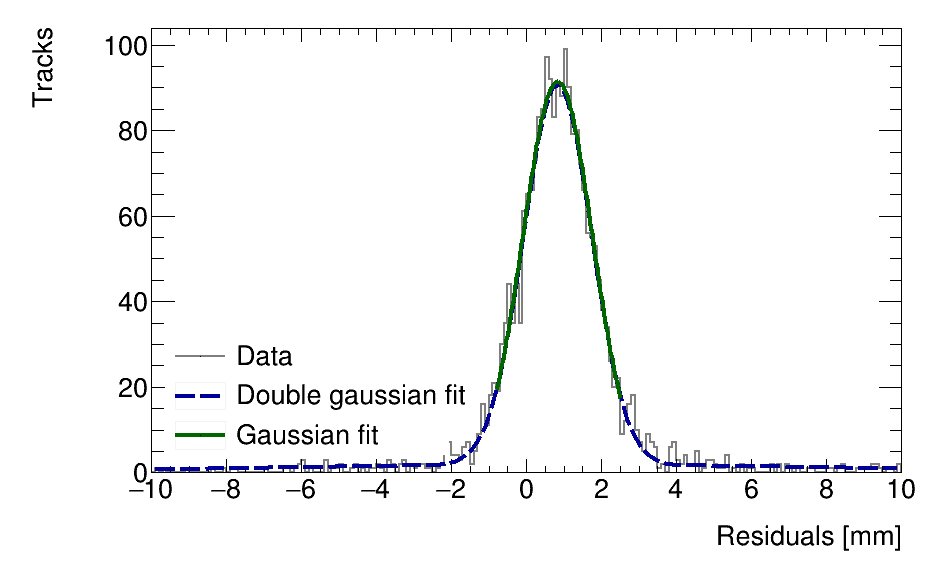
\includegraphics[width = \textwidth]{figures/figure_double_gaussian_quick_and_dirty_2900V_log_scale_gaussian_QL2C04_2900V_2021-02-08_2_xbin_10_ybin_5_100mm.png}
    \caption{Residual distribution for tracks on layer 1 built from hits on layers 3 and 4 for $x\in\left[-3.00, 97.00\right],  y\in\left[394.60, 494.60\right] mm$ for QL2.C.4 fit with a double gaussian and a single gaussian in a range of $\pm$1 RMS from the histogram mean.}
    \label{fig:double_gaussian_example_fit}
\end{figure}

For all residual distributions in \SI{100}{\milli\meter} by \SI{100}{\milli\meter} bins on layer 1 built from hits on layers 3 and 4, the difference in gaussian and double gaussian means and $\sigma$'s is shown in figure \ref{fig:double_gaussian_compare_fits}. Since the RMS of the residual mean differences distribution is less than \SI{50}{\micro\meter} the gaussian fit gave the same result within the required precision. Moreover, this is for the tracking combination with the worst extrapolation lever arm and the widest distribution of mean differences; the interpolation combinations have narrower distributions. 

The gaussian $\sigma$ should be larger than the double gaussian $\sigma$ because the gaussian distribution includes the effect of the noise tracks with large residuals, while the double gaussian models signal and background residuals separately. For this analysis, only the residual mean was important, so the systematic overestimate of the signal $\sigma$ in the gaussian fit shown on the right of figure \ref{fig:double_gaussian_compare_fits} was allowed.

\begin{figure}
    \centering
    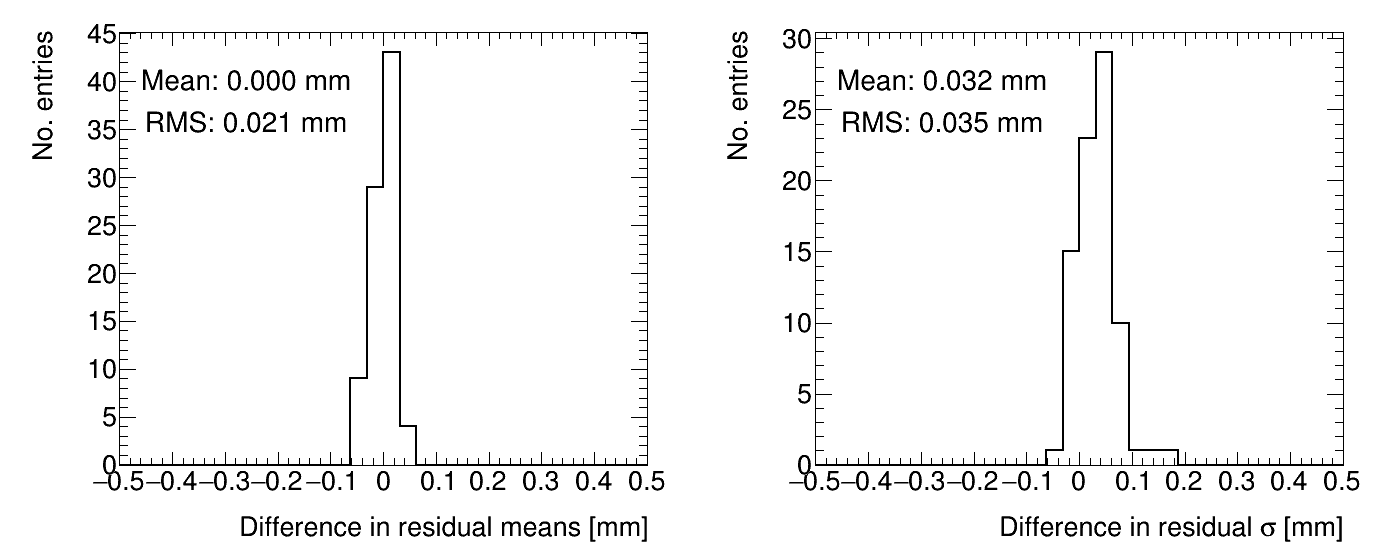
\includegraphics[width = \textwidth]{figures/figure_compare_residual_fits_QL2C04_2900V_2021-02-08_2_fit_range_mean_pm_RMS_minus_quick_and_dirty_2900V_log_scale_layer1_fixedlayers34.png}
    \caption{Difference in residual distribution means and $\sigma$'s for a gaussian and double gaussian fit, for all residual distributions in \SI{100}{\milli\meter} by \SI{100}{\milli\meter} bins on layer 1 built from hits on layers 3 and 4 for QL2.C.4, data taken at 2900 V.}
    \label{fig:double_gaussian_compare_fits}
\end{figure}

% --------------------------------------------------
\section{Area of residual distribution regions of interest}
% --------------------------------------------------
\label{appendix:systematics_bin_size}
% Edit count: 1
% DO I NEED TO EXPLAIN THIS IN MATH? I tried on June 3rd in my notes, it's complicated for such a simple thing.
% If this flies, you'll need to establish that reference frame == two fixed layers' frame as jargon in your thesis.
% Also need to establish x == perpendicular to wires; y == perpendicular to strips. ==> How do I do this consistently?
% May need to add 3100V reference if it's not already defined in your thesis.
% Define ROI as short form?

%TODO : How do I cite the distribution of rotations angles by Dylan?
The area of the region of interest in which to include tracks is primarily motivated by the misalignment model: the width of the region should be less than the scale on which the local offset is expected to change significantly. Changes in offset of order \SI{50}{\micro\meter}, the approximate position resolution of the sTGCs in the $\eta$-coordinate, are significant. In a misalignment model with an offset and rotation, only the rotation changes the local offset with respect to the x-coordinate \footnote{The effect of rotation can be modeled by assuming the recorded track position is related to the hit position by a passive rotation. The angle of rotation is the relative angle between the layer of interest and the nominal geometry. The local offset does change with respect to the track's y coordinate as well, but negligibly in the limit of small rotation angles.}.  The distribution of the as-built cathode board rotation angles shows that the RMS of the rotation angle is \SI{200}{\micro\radian} [https://indico.cern.ch/event/1035057/ PG. 18]; however, the distribution has a long tail so a typical rotation angle of \SI{1000}{\micro\radian} was used here. A rotation of \SI{1000}{\micro\radian} will cause a \SI{50}{\micro\meter} change in local offset over a change in x of \SI{50}{\centi\meter}. Therefore, the width of the region of interest should be less than \SI{500}{\milli\meter}.

Two other factors inform the width of the region. First, since the hits' x-coordinates are discrete the width in x must be larger than the pitch of the wire groups to ensure the bin will have a sufficient number of tracks fall in it. Second, more tracks will be included in a larger area so more statistics will be available for the residual distribution fit. For the bin widths wider than two wire groups, the statistics are sufficient. For each x-ray residual, the mean cosmics residual was calculated for a few different bin widths, and the difference in means plotted. Figure \ref{fig:area_bin_size_mean_diff} shows an example for QL2.C.4. The width of the distribution is on the order of \SI{50}{\micro\meter}, showing that the calculation of the residual mean is relatively robust with respect to the area of the bin. However, \SI{50}{\micro\meter} is greater than the typical statistical uncertainty on the cosmic residual of means, which ranges from \SI{10}{\micro\meter} - \SI{40}{\micro\meter} depending on the tracking combination under study. Therefore, the cosmic residual means are assigned an uncertainty of \SI{50}{\micro\meter}.
%TODO : Verity that you actually apply the 50 um uncertainty.

%TODO : This figure should have the mean and rms on it.
\begin{figure}
    \centering
    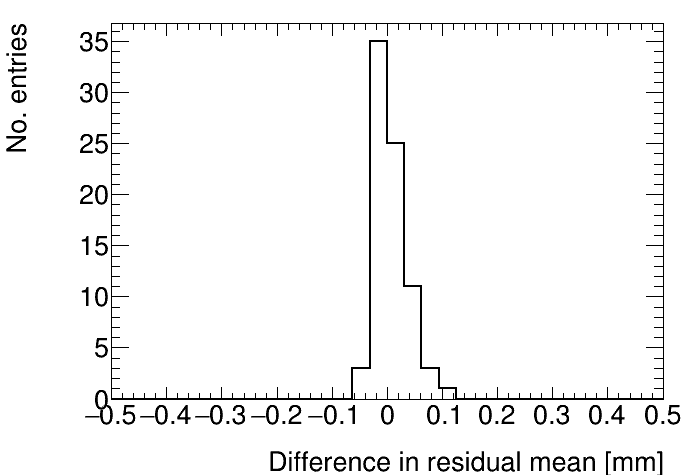
\includegraphics[width = \textwidth]{figures/compare_residual_fits_around_xrays_QL2C04_3100V_2021-05-20_100mm_width_bins_minus_QL2C04_3100V_2021-06-02_200mm_width_bins_means_difference.png}
    \caption{Difference in cosmic residual means around x-ray residuals for square bins of 100 mm width and 200 mm width for QL2.C.4.}
    \label{fig:area_bin_size_mean_diff}
\end{figure}

For this analysis, \SI{100}{\milli\meter} by \SI{100}{\milli\meter} by \SI{100}{\milli\meter} bins were used.

% --------------------------------------------------
\section{Differential non-linearity}
% --------------------------------------------------
\label{appendix:systematics_dnl}
% Edit count: 1
In this context, differential non-linearity (DNL) is when the reconstructed cluster mean is biased by the fit of the discretely sampled PDO distribution over the strips. The bias depends on the relative position of the avalanche with respect to the center of the closest strip. For a summary of DNL, refer to page 40 of Lefebvre's thesis \cite{lefebvre_thesis}. The cluster mean was corrected for DNL using the equation:
\begin{equation}
\label{eqn:dnl_corr}
y' = y + a \sin \left( 2 \pi y_{rel} \right)
\end{equation}

where $y$ is the cluster mean, $y_{rel}$ is the relative position of the cluster mean with respect to the strip's center, $a$ is the amplitude of the correction, and $y'$ is the corrected cluster mean. The amplitude can be derived by comparing the reconstructed hit position to the expected hit position, as done in Abusleme, 2016 \cite{abusleme_performance_2016}. With cosmic muons, there is no reference hit position to compare to, so track residuals were used as a proxy \cite{lefebvre_thesis}. The hallmark of the DNL effect is the periodic pattern in the residual versus $y_{rel}$ profile, and the effect of correcting the cluster means using an amplitude of \SI{50}{\micro\meter} is shown in figure \ref{fig:dnl_corr_effect}. An amplitude of \SI{50}{\micro\meter} was based on Lefebvre's estimate of the DNL amplitudes by layer, quadruplet and cluster size using exclusive cosmic muon tracks in \package{tgc\_analysis/CosmicsAnalysis}. Little variation was seen in the amplitude parameters with respect to the quadruplet tested, the layer and the cluster size so a universal correction was used.
%TODO How little is little? Check your notes.
%TODO exclusive better be defined somewhere clearly.

\begin{figure}
    \centering
    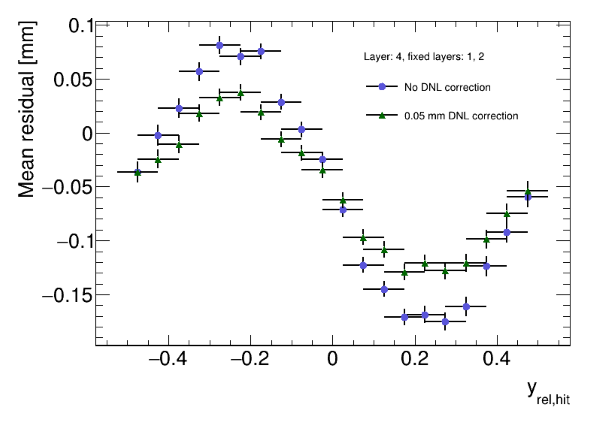
\includegraphics[width = \textwidth]{figures/figure_dnl_profiles_blue_QL2P08_3100V_2021-06-18_no_dnl_green_QL2P08_3100V_2021-06-18_2_50um_universal_DNL_layer4_fixed12.png}
    \caption{Effect applying a \SI{50}{\micro\meter} DNL correction to the cluster means on the residual vs $y_{rel}$ distribution for tracks built from layers 1 and 2 and extrapolated to layer 4 for QL2.P.8.}
    \label{fig:dnl_corr_effect}
\end{figure} 

Although the correction is not large enough in this case, the figure shows that the correction does reduce the DNL effect. Slightly better performance is seen in the interpolation tracking combinations where the quality of the residuals is better. DNL corrections for cosmic muon data are difficult because the DNL effect is obscured by the effect of misalignments and noise. Misalignments cause the center of the sine pattern in figure \ref{fig:dnl_corr_effect} to be shifted off of zero, since the mean of residuals is shifted.

In figure \ref{fig:dnl_compare_fits}, it is apparent that the effect of the DNL correction on the mean of the residual distribution in \SI{100}{\milli\meter} by \SI{100}{\milli\meter} areas is on the order of micrometers in the worst extrapolation case. Although the $\sigma$'s of the residual distributions shrink with the DNL correction, the mean is the parameter of interest. Therefore, for this analysis DNL was not corrected for.

\begin{figure}
    \centering
    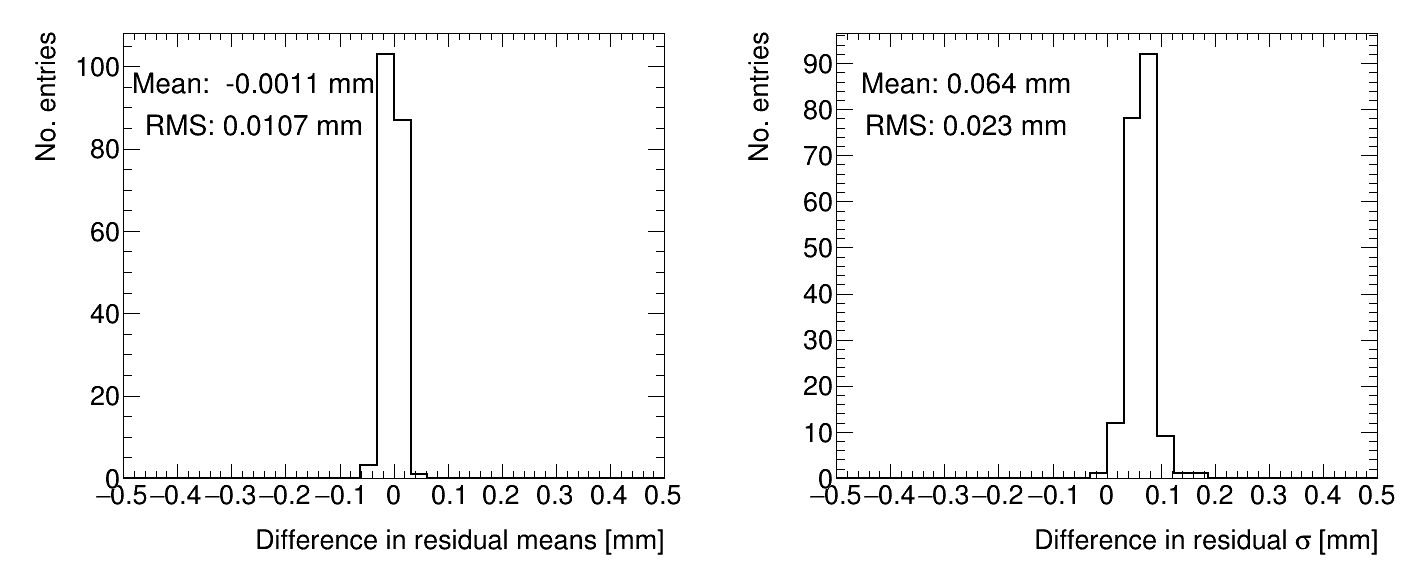
\includegraphics[width = \textwidth]{figures/figure_compare_residual_fits_QL2P08_3100V_2021-06-18_no_dnl_minus_QL2P08_3100V_2021-06-18_2_50um_universal_DNL_layer4_fixedlayers12.png}
    \caption{Difference in residual distribution means and $\sigma$'s with and without DNL correction for residuals on layer 4 from reference layers 1 and 2 for QL2.P.8.}
    \label{fig:dnl_compare_fits}
\end{figure}
































% ==================================================
% Appendix: Printable plots %
% ==================================================

\chapter[Printable plots]{Printable plots}
\label{appendix:print}
% Edit count: 0

\begin{figure}
    \centering
    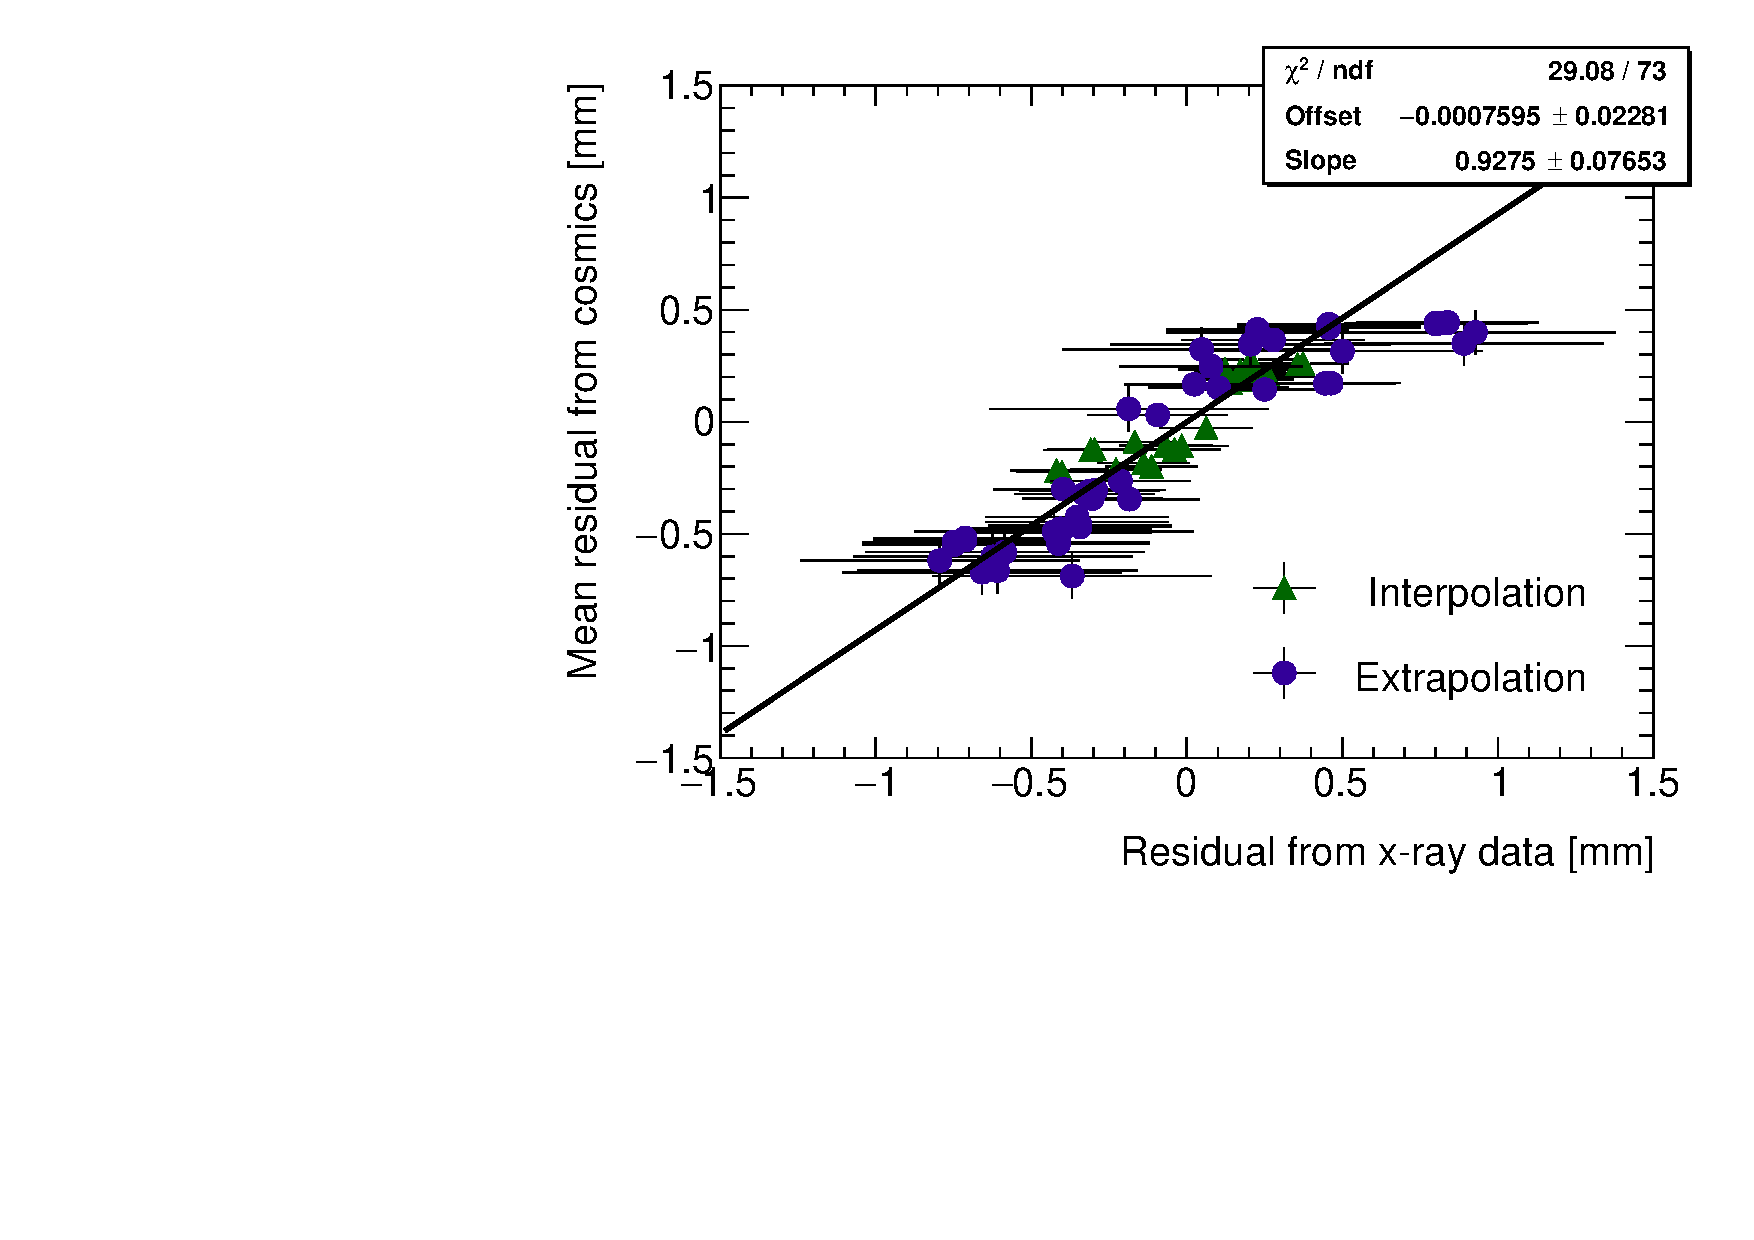
\includegraphics[width = \textwidth]{figures/figure_QL2P11_3100V_2021-08-05_QL2P11_local_cosmic_and_xray_data_correlation_plot_printable.pdf}
    \caption{Correlation plot between x-ray and cosmics residuals for all tracking combinations for QL2.P.11. Each rectangle is centered on an x-ray and mean cosmics residual pair. The width of the rectangles in $x$ and $y$ are the uncertainty in the x-ray and mean cosmics residual respectively. A printable version of figure~\ref{fig:correlation} in section~\ref{sec:assessing_correlation}.}
    \label{fig:correlation_print}
\end{figure}

\begin{figure}
    \centering
    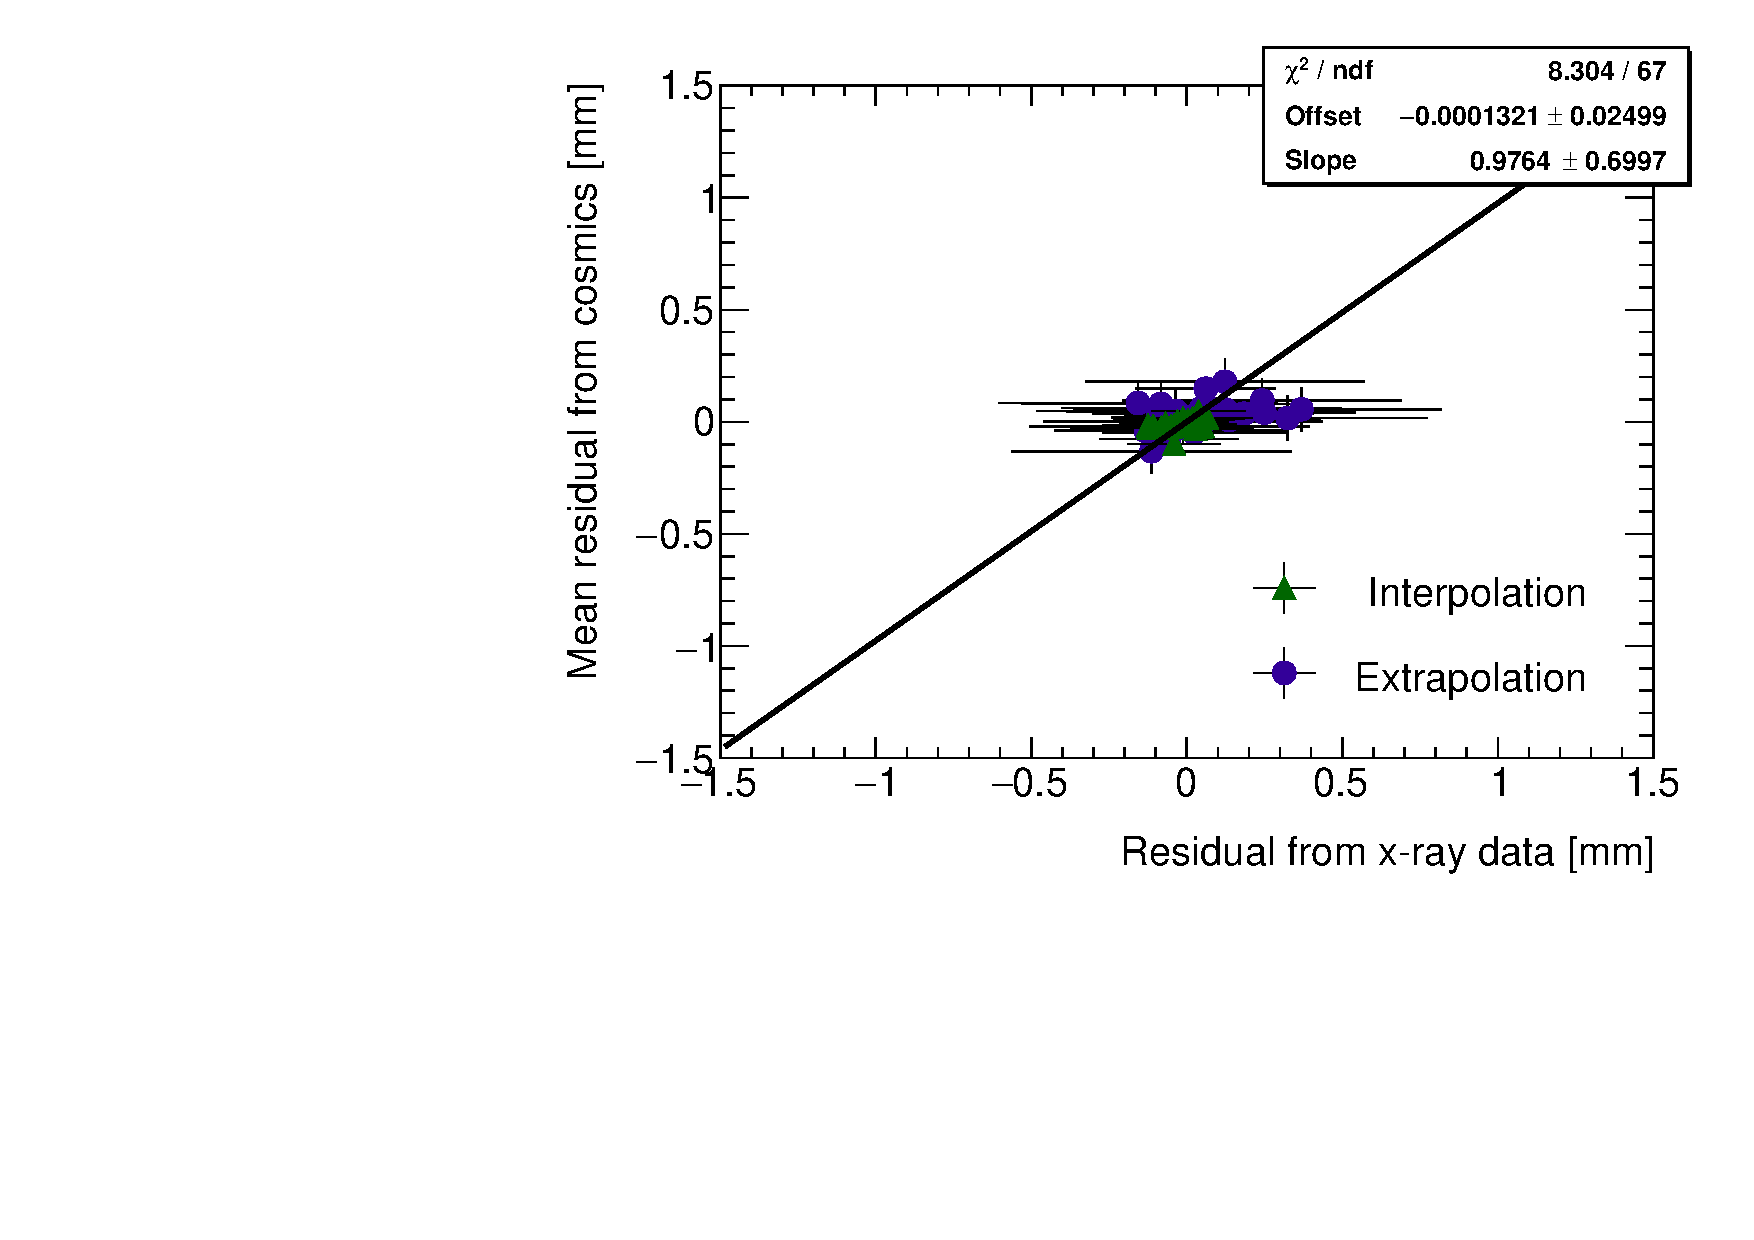
\includegraphics[width = \textwidth]{figures/figure_QL2P08_3100V_2021-08-16_QL2P08_local_cosmic_and_xray_data_correlation_plot_printable.pdf}
    \caption{Correlation plot between x-ray and cosmics residuals for all tracking combinations for QL2.P.8. Each rectangle is centered on an x-ray and mean cosmics residual pair. The width of the rectangles in $x$ and $y$ are the uncertainty in the x-ray and mean cosmics residual respectively. A printer friendly version of this plot is available. A printable version of figure~\ref{fig:no_correlation} in section~\ref{sec:assessing_correlation}.}
    \label{fig:no_correlation_print}
\end{figure}

% GLOSSARIES (Lists of definitions, abbreviations, symbols, etc. provided by the glossaries-extra package)
% -----------------------------
% \printglossaries
% \cleardoublepage
% \phantomsection		% allows hyperref to link to the correct page

%----------------------------------------------------------------------
\end{document} % end of logical document
